\chapter{Transfer, Generators and Localized Training}
\label{ch:generators}

\section{The transfer theorem}\label{m:sec:main}

Chapters~\ref{ch:manifold} and~\ref{ch:adjoint} state the Bernstein von Mises theorems of Nickl~\cite{nicklbvm2024} and of Konen and Nickl~\cite{konennickl2026} for the exact posterior of the initial condition and reduce the data to a statistic of dimension $J_N$ that is exactly sufficient for linear equations and, under Assumption~\ref{m:ass:U}, sufficient at the scale $N^{-1/2}$ for nonlinear ones. Algorithm~\ref{m:alg:gbc} does not sample the exact posterior. It samples the output of a generator trained on $M$ simulated pairs, and nothing proved so far says that this output shares the guarantees. This chapter asks how accurate the generator must be for the guarantees to pass to its output, whether a concrete generator is that accurate at a simulation budget one can pay, and how the training pairs should be drawn.

The first answer is Theorem~\ref{m:thm:main}. If the Wasserstein distance between the GBC posterior and the exact posterior is $o(N^{-1/2})$, and the GBC posterior concentrates on the localization set (Assumption~\ref{m:ass:G}), then it has the same Gaussian limit as the exact posterior for the initial condition and, for the equations covered by the theorems of Nickl and of Konen and Nickl, for the trajectory; its credible bands have exact asymptotic coverage; and for the Navier Stokes equations the solution started at its mean is a regular estimator of the state that attains the local asymptotic minimax bound for bounded losses. Nothing is assumed about how the generator was trained. The second answer has two halves. An identity skip generator with a Gaussian head computed in closed form meets the accuracy requirement as soon as $J_N/M_N\to0$ (Theorem~\ref{m:thm:qnnA}), but only conditionally on Assumptions~\ref{m:ass:U} and~\ref{m:ass:u2p} and on a bound for the error of the summary (Open Question~\ref{m:op:unif}). A generator required to be accurate uniformly over a H\"older class of quantile maps cannot meet the requirement with polynomially many simulations once the dimension of the summary grows (Theorem~\ref{m:thm:qnnB}). The third answer concerns the training distribution, which matters as much as the architecture: Section~\ref{m:sec:loc} computes the exact law of the residual under a localized proposal in the linear Gaussian model and derives from it a training rule, which is to center the residuals and rescale them, and explains why importance weighting back to the prior is not used.

Let $\Wone_1=\Wone_{1,H^{-k-2}}$ with $k$ as in Theorem~\ref{m:thm:nickl2}. The localization set of Theorem~3 in Nickl~\cite{nicklbvm2024} is contained in an intersection of a Sobolev ball with Sobolev neighborhoods of $\theta_0$, and that containment is all the proof below uses of it, so we write $\bar\Theta_{N,L}$ for the intersection:
\begin{equation}\label{m:eq:locset}
\begin{aligned}
\bar\Theta_{N,L}&=\{\norm\theta_{H^{\bar\gamma}}\le L\}\cap\big\{\norm{\theta-\theta_0}_{H^\xi}\le L\tilde\delta_N(\xi)\ \ \forall\,0\le\xi<\bar\gamma\big\},\\
\tilde\delta_N(\xi)&=\delta_N^{(\bar\gamma-\xi)/(\bar\gamma+1)},
\end{aligned}
\end{equation}
where $\bar\gamma$ is the Sobolev index of the localization ball, chosen as in the cited proofs within $\max(2,2\zeta)<\bar\gamma<\gamma-\max(1,d/2)$, a nonempty range under the hypothesis $\gamma>\max(3\zeta+3d/2+2,\eta_0)$ of Theorem~\ref{m:thm:nickl2}. Two constants of the proof being transferred enter the hypotheses below. The first is the exponent $m$ in the linearization bound
\begin{equation}\label{m:eq:interpm}
\begin{aligned}
&\norm{u_\theta-u_\vartheta-\I_{\theta_0}[\theta-\vartheta]}_\Ccal\ \lesssim\ \big(\norm{\theta-\theta_0}^2_{L^2}+\norm{\vartheta-\theta_0}^2_{L^2}\big)^m,\\
&\qquad \norm\theta_{H^{\bar\gamma}}\vee\norm\vartheta_{H^{\bar\gamma}}\le M ,
\end{aligned}
\end{equation}
which arises from interpolating $L^2$ against $H^{\bar\gamma}$ and is therefore always at most $1$: it is $m=(\bar\gamma-\zeta)/\bar\gamma$ with $d/2<\zeta<\bar\gamma$ in Nickl~\cite{nicklbvm2024} and $m=(\bar\gamma-1)/\bar\gamma$ in Konen and Nickl~\cite{konennickl2026}. It is also strictly greater than $1/2$, since those proofs need $\tilde\delta_N^{2m}=o(N^{-1/2})$ while $\tilde\delta_N\ge N^{-1/2}$ (Remark~\ref{m:rem:jwmeasure}), so that $N^{-m}=o(N^{-1/2})$. That requirement is stronger than $m>1/2$ and is what restricts the choice of $\bar\gamma$ and $\zeta$ in the range above: it forces $\bar\gamma>2\zeta+1$. The second is the moment order
\begin{equation}\label{m:eq:qorder}
\begin{gathered}
q=4\ \ \text{in the setting of Theorem~\ref{m:thm:nickl1}},\\
q=4\bar\gamma\ \ \text{in that of Theorem~1.1 of Konen and Nickl~\cite{konennickl2026}},
\end{gathered}
\end{equation}
which is what the two Cauchy Schwarz steps of that proof consume.

\begin{assumption}[GBC accuracy]\label{m:ass:G}
As $N\to\infty$, in $P^\N_{\theta_0}$ probability:
\begin{enumerate}[label=(G\arabic*),nosep]
\item $\sqrt N\,\Wone_1(\Pihat,\PiN)\to0$.
\item For some $b>0$ and $L$, $\Pihat(\bar\Theta_{N,L}^c)\le e^{-bN\delta_N^2}$, and $E^{\Pihat}\norm\theta^{q}_{H^{\bar\gamma}}=O_P(1)$ with $q$ as in \eqref{m:eq:qorder}.
\end{enumerate}
\end{assumption}

Because $q\ge4$ and $\bar\gamma\ge2$, the moment clause of (G2) contains the bound $E^{\Pihat}\norm\theta^2_{H^2}=O_P(1)$ used elsewhere, and adds the two things the proof of part (ii) needs and that a second moment does not give: the moment of order $4m<4$ consumed by the Cauchy Schwarz step off $\bar\Theta_{N,L}$, and, through Jensen's inequality, $\norm{\hat\theta^{\rm G}_N}_{H^{\bar\gamma}}\le(E^{\Pihat}\norm\theta^q_{H^{\bar\gamma}})^{1/q}=O_P(1)$. The clause is the analogue for $\Pihat$ of the posterior moment bound (39) of Nickl~\cite{nicklbvm2024}, namely $(E^{\PiN}\norm{\theta-\theta_0}^r_{H^\xi})^{1/r}=O_P(\tilde\delta_N(\xi))$ for every $r<\infty$ and every $0\le\xi\le\bar\gamma$, which holds at every order for the exact posterior and at no order for a learned measure: that is why it has to be assumed rather than derived. It can, however, be enforced by construction rather than assumed, by composing the generator with the radial retraction $r(\theta)=\theta\min(1,L/\norm\theta_{H^{\bar\gamma}})$ onto the ball $B_L=\{\norm\theta_{H^{\bar\gamma}}\le L\}$, with $L$ the constant of (G2). The clause then holds at every order trivially. The first clause of (G2) survives with $2e^{-bN\delta_N^2}$ in place of $e^{-bN\delta_N^2}$, because $r$ is the identity on $B_L\supset\bar\Theta_{N,L}$, and so does (G1): with $s=K_N/\sqrt N$ and the $1$ Lipschitz function $\phi_s(\theta)=(\norm{\theta-\theta_0}_{H^{-k-2}}-s)_+$,
\[
\begin{aligned}
\Wone_1(r_\#\Pihat,\Pihat)&\le E^{\Pihat}\big[\norm\theta_{H^{-k-2}}\mathbf 1_{B^c_L}\big]\\
&\le\big(s+\norm{\theta_0}_{H^{-k-2}}\big)\Pihat(B^c_L)+E^{\PiN}\phi_s+\Wone_1(\Pihat,\PiN),
\end{aligned}
\]
and each term is $o_P(N^{-1/2})$ for $K_N\to\infty$ slowly: the first by the first clause of (G2), the second by the uniform integrability of $\norm{\sqrt N(\theta-\theta_0)}_{H^{-k-2}}$ under $\PiN$ that the convergence in $\Wone_1$ of Theorem~\ref{m:thm:nickl2} gives, and the third by (G1). So the retraction costs nothing asymptotically. The proof of Theorem~\ref{m:thm:qnnA} discharges it for the plug in Gaussian generator of Definition~\ref{m:def:gen}, so the strengthening costs that theorem nothing.

Under Assumption~\ref{m:ass:U}, (G1) holds for the exact generator with the posterior mean summary by Corollary~\ref{m:cor:jwgbc}, and for the one step summary by Proposition~\ref{m:prop:suff} together with the last statement of Theorem~\ref{m:thm:jwbvm}, which needs the same assumption; the generator's estimation error is the remaining contribution and is the subject of Section~\ref{m:sec:qnn}.

\begin{theorem}[BvM for GBC]\label{m:thm:main}
Suppose Conditions 1 and 2 of Nickl~\cite{nicklbvm2024} hold with the constants of Theorem~\ref{m:thm:nickl2}, and Assumption~\ref{m:ass:G} holds. Then:
\begin{enumerate}[label=(\roman*),nosep]
\item $\Wone_1\big(\Law(\sqrt N(\theta-\hat\theta_N^{\rm G})\mid\theta\sim\Pihat),\,\Ncal_{\theta_0}\big)\to^{P}0$ and $\sqrt N(\hat\theta_N^{\rm G}-\theta_0)\to^d\Ncal_{\theta_0}$ in $H^{-k-2}$.
\item If in addition the forward map satisfies the hypotheses of Theorem~\ref{m:thm:nickl1} or of Theorem~1.1 in Konen and Nickl~\cite{konennickl2026}, then
\[
\begin{gathered}
\Wone_{1,\Ccal}\big(\Law(\sqrt N(u_\theta-u_{\hat\theta_N^{\rm G}})\mid\theta\sim\Pihat),\,\mu\big)\to^P0,\\
\sqrt N\big(u_{\hat\theta_N^{\rm G}}-u_{\theta_0}\big)\to^d_\Ccal\mu .
\end{gathered}
\]
\item For $\Phi:\Ccal\to\mathbb B$ Hadamard differentiable, $\sqrt N(\Phi(u_{\hat\theta_N^{\rm G}})-\Phi(u_{\theta_0}))\to^d\dot\Phi_{u_{\theta_0}}[U]$, and the GBC credible band $C^{\rm G}_N$ of $\Pihat$ probability $1-\beta$ satisfies $P^\N_{\theta_0}(u_{\theta_0}\in C^{\rm G}_N)\to1-\beta$, its radius $R_N$ in $\Ccal$ obeying $\sqrt NR_N\to c>0$.
\item In the Navier Stokes case of (ii), write $\theta_{N,h}=\theta_0+h/\sqrt N$. Then for every $h\in\Hds\infty$, under $P^\N_{\theta_{N,h}}$,
\[
\sqrt N\big(\hat\theta^{\rm G}_N-\theta_{N,h}\big)\to^d\Ncal_{\theta_0}\ \text{ in }H^{-k-2},\qquad \sqrt N\big(u_{\hat\theta^{\rm G}_N}-u_{\theta_{N,h}}\big)\to^d_\Ccal\mu ;
\]
that is, $u_{\hat\theta^{\rm G}_N}$ is a regular estimator sequence of the state at $\theta_0$, with the limit law $\mu$ that attains the bound of Theorem~1.2 in Konen and Nickl~\cite{konennickl2026} (Theorem~2.10 there for a general $\Phi$). Consequently, with $\Phi$ as in (iii) and $\Phi=\Id$ permitted, $\Phi(u_{\hat\theta^{\rm G}_N})$ is efficient among regular estimator sequences by the convolution theorem, and for every bounded, continuous, subconvex loss $\ell:\mathbb B\to[0,\infty)$ it attains the local asymptotic minimax bound,
\[
\begin{aligned}
&\sup_{J\subset\Hds\infty,\ |J|<\infty}\ \liminf_{N\to\infty}\ \max_{h\in J}\ E^\N_{\theta_{N,h}}\,\ell\Big(\sqrt N\big(\Phi(u_{\hat\theta^{\rm G}_N})-\Phi(u_{\theta_{N,h}})\big)\Big)\\
&\qquad=\ E_\mu\,\ell\big(\dot\Phi_{u_{\theta_0}}[U]\big),\qquad U\sim\mu .
\end{aligned}
\]
\end{enumerate}
\end{theorem}

\begin{proof}
Three facts about $\Wone_1$ on a separable Banach space $B$: (a) translation invariance; (b) $\Wone_1(\Law(cX),\Law(cY))=|c|\Wone_1(\Law X,\Law Y)$; (c) $\norm{EX-EY}_B\le\Wone_1(\Law X,\Law Y)$, since $x\mapsto\langle x,\psi\rangle$ is Lipschitz with constant $1$ for $\psi$ in the dual unit ball.

(i) With $\tau^{\rm G}_N$, $\tau'_N$, $\tau_N$ the laws of $\sqrt N(\theta-\hat\theta^{\rm G}_N)$ under $\Pihat$, of $\sqrt N(\theta-\hat\theta^{\rm G}_N)$ under $\PiN$, and of $\sqrt N(\theta-\tilde\theta_N)$ under $\PiN$,
\[
\Wone_1(\tau_N^{\rm G},\Ncal_{\theta_0})\le\Wone_1(\tau_N^{\rm G},\tau_N')+\Wone_1(\tau_N',\tau_N)+\Wone_1(\tau_N,\Ncal_{\theta_0}).
\]
By (a) and (b) the first term is $\sqrt N\Wone_1(\Pihat,\PiN)\to^P0$ by (G1); the second is at most $\sqrt N\norm{\tilde\theta_N-\hat\theta^{\rm G}_N}_{H^{-k-2}}\le\sqrt N\Wone_1(\Pihat,\PiN)$ by (a) and (c); the third tends to zero by Theorem~\ref{m:thm:nickl2}. The mean statement follows by Slutsky in $H^{-k-2}$.

(ii) Follow the proof of Theorem~1 in Nickl~\cite{nicklbvm2024}, or of Theorem~1.1 in Konen and Nickl~\cite{konennickl2026}, with $\PiN$ replaced by $\Pihat$ and $\tilde\theta_N$ by $\hat\theta^{\rm G}_N$. The term $\sup_{\norm F_{\Lip}\le1}|EF(\I_{\theta_0}Z^{\rm G}_N)-EF(\I_{\theta_0}Z)|$, in which $Z^{\rm G}_N$ has the law $\Law(\sqrt N(\theta-\hat\theta^{\rm G}_N)\mid\theta\sim\Pihat)$ and $Z\sim\Ncal_{\theta_0}$, is at most $\Lip(\I_{\theta_0}:H^{-k-2}\to\Ccal)$ times the quantity in (i). The linearization term $\sqrt N\,E^{\Pihat}\norm{u_\theta-u_{\hat\theta^{\rm G}_N}-\I_{\theta_0}[\theta-\hat\theta^{\rm G}_N]}_\Ccal$ is handled by that argument, which uses three properties of the measure it integrates against and nothing else.

\emph{(a) The centering lies in a fixed Sobolev ball.} The argument is run on the frequentist event $\{\norm{\hat\theta^{\rm G}_N}_{H^{\bar\gamma}}\le M\}$, on which \eqref{m:eq:interpm} may be applied with $\vartheta=\hat\theta^{\rm G}_N$. By Jensen and the moment clause of (G2), $\norm{\hat\theta^{\rm G}_N}_{H^{\bar\gamma}}\le(E^{\Pihat}\norm\theta^q_{H^{\bar\gamma}})^{1/q}=O_P(1)$, so that event has probability tending to one for $M$ large; for the exact posterior the same is (39) of Nickl~\cite{nicklbvm2024} at $\xi=\bar\gamma$.

\emph{(b) Exponentially small mass off the ball, with a moment for the integrand there.} By \eqref{m:eq:locset}, $\bar\Theta_{N,L}\subset B_L:=\{\norm\theta_{H^{\bar\gamma}}\le L\}$, so the first clause of (G2) gives $\Pihat(B^c_L)\le e^{-bN\delta_N^2}$. On $B^c_L$ the integrand is at most a constant times $1+\norm\theta_{H^2}$ in the setting of Theorem~\ref{m:thm:nickl1}, by $\sup_t\norm{u_\theta(t)}^2_{H^2}\lesssim1+\norm\theta^2_{H^2}$ and the embedding $H^2\subset C(\Omega)$ for $d\le3$, and at most a constant times $1+\norm\theta^{2\bar\gamma}_{\Hds{\bar\gamma}}$ in that of Konen and Nickl~\cite{konennickl2026}. Cauchy Schwarz and (G2) bound its contribution by
\[
\big(E^{\Pihat}\big[1+\norm\theta^{q}_{H^{\bar\gamma}}\big]\big)^{1/2}\,\Pihat(B^c_L)^{1/2}=O_P(1)\,e^{-bN\delta_N^2/2}=o_P(N^{-1/2}),
\]
since $N\delta_N^2=N^{d/(2\gamma+d)}$ is a positive power of $N$. This is what fixes $q$ in \eqref{m:eq:qorder}.

\emph{(c) On the ball, the linearization bound \eqref{m:eq:interpm}}, for which one needs $E^{\Pihat}\norm{\theta-\theta_0}^{2m}_{L^2}=o_P(N^{-1/2})$ and $\norm{\hat\theta^{\rm G}_N-\theta_0}_{L^2}=O_P(\tilde\delta_N)$. For the exact posterior the first is (39) of Nickl~\cite{nicklbvm2024} at order $2m$; for $\Pihat$ we have only (G2), and split at $\bar\Theta_{N,L}$. By \eqref{m:eq:locset}, $\bar\Theta_{N,L}\subset\{\norm{\theta-\theta_0}_{L^2}\le L\tilde\delta_N\}$, so
\[
E^{\Pihat}\norm{\theta-\theta_0}^{2m}_{L^2}\ \le\ L^{2m}\tilde\delta_N^{2m}+\big(E^{\Pihat}\norm{\theta-\theta_0}^{4m}_{L^2}\big)^{1/2}\,\Pihat(\bar\Theta^c_{N,L})^{1/2} .
\]
The first term is $o(N^{-1/2})$ by the choice of $\bar\gamma$ and $\zeta$ in the cited proofs. The second is $O_P(1)e^{-bN\delta_N^2/2}$: since $4m<4\le q$ and $\norm\cdot_{L^2}\le\norm\cdot_{H^{\bar\gamma}}$, Lyapunov's inequality and (G2) give
\[
\begin{aligned}
E^{\Pihat}\norm{\theta-\theta_0}^{4m}_{L^2}&\le\big(E^{\Pihat}\norm{\theta-\theta_0}^{q}_{H^{\bar\gamma}}\big)^{4m/q}\\
&\lesssim\big(E^{\Pihat}\norm{\theta}^{q}_{H^{\bar\gamma}}+\norm{\theta_0}^{q}_{H^{\bar\gamma}}\big)^{4m/q}=O_P(1) .
\end{aligned}
\]
It is this step, and only this step, that a second moment does not cover: $4m>2$ whenever $m>1/2$, and $m>1/2$ is forced. Finally, Jensen and $2m\ge1$ give $\norm{\hat\theta^{\rm G}_N-\theta_0}_{L^2}\le E^{\Pihat}\norm{\theta-\theta_0}_{L^2}\le(E^{\Pihat}\norm{\theta-\theta_0}^{2m}_{L^2})^{1/(2m)}=O_P(\tilde\delta_N)$. The single point statement uses (i) and continuity of $\I_{\theta_0}$.

(iii) The delta method is Section~3.10 of van der Vaart and Wellner~\cite{vandervaartwellner2023}. Coverage follows from (ii) as Corollary~1.3 of Konen and Nickl~\cite{konennickl2026} follows from their Theorem~1.1, via Theorem~7.3.23 of Gin\'e and Nickl~\cite{ginenickl2016}: $t\mapsto\mu(\norm U_\Ccal\le t)$ is continuous and strictly increasing because $\mu$ is nondegenerate (Section~2.6 of Konen and Nickl~\cite{konennickl2026} for Navier Stokes, Lemma~\ref{m:lem:nondeg} for the reaction diffusion class), $\Wone_{1,\Ccal}$ convergence gives convergence of the $\Pihat$ quantiles of $\norm{Y^{\rm G}_N}_\Ccal$, in which $Y^{\rm G}_N=\sqrt N(u_\theta-u_{\hat\theta^{\rm G}_N})$ with $\theta\sim\Pihat$, and $\sqrt N\norm{u_{\hat\theta^{\rm G}_N}-u_{\theta_0}}_\Ccal\to^d\norm U_\Ccal$.

(iv) Recall that the design is uniform on $\mathcal X=[0,T]\times\Omega$, a set of measure $T$, so that $E\norm{g(X)}^2_W=T^{-1}\norm g^2_{L^2(\mathcal X)}$ with $L^2(\mathcal X)$ unnormalized.

\emph{Step 1: local asymptotic normality at $\theta_0$.} In the Gaussian model \eqref{m:eq:model} the log likelihood ratio is exactly
\[
\begin{aligned}
\Lambda_N(h)&:=\log\frac{dP^\N_{\theta_{N,h}}}{dP^\N_{\theta_0}}\big(Z^{(N)}\big)=\sum_{i=1}^N\Big[\big\langle\varepsilon_i,\Delta_N(X_i)\big\rangle_W-\tfrac12\norm{\Delta_N(X_i)}^2_W\Big],\\
\Delta_N&=\Gcal(\theta_{N,h})-\Gcal(\theta_0).
\end{aligned}
\]
Condition 2C gives $\norm{\Delta_N-\I_{\theta_0}[h]/\sqrt N}_{L^2(\mathcal X)}\lesssim\norm h^2_{L^2}/N$, so the linear part differs from $N^{-1/2}\sum_i\langle\varepsilon_i,\I_{\theta_0}[h](X_i)\rangle_W$ by a centered term of variance $NT^{-1}\norm{\Delta_N-\I_{\theta_0}[h]/\sqrt N}^2_{L^2(\mathcal X)}=O(N^{-1})$, and Condition 2D makes $\I_{\theta_0}[h]$ bounded, so $\sum_i\norm{\Delta_N(X_i)}^2_W\to^PT^{-1}\norm{\I_{\theta_0}h}^2_{L^2(\mathcal X)}$. Hence
\[
\begin{aligned}
\Lambda_N(h)&=\frac1{\sqrt N}\sum_{i=1}^N\big\langle\varepsilon_i,\I_{\theta_0}[h](X_i)\big\rangle_W-\frac{\sigma^2_h}{2}+o_P(1)\ \to^d\ N\Big(-\frac{\sigma^2_h}{2},\,\sigma^2_h\Big),\\
\sigma^2_h&=\frac1T\norm{\I_{\theta_0}h}^2_{L^2(\mathcal X)} .
\end{aligned}
\]
The experiment is therefore locally asymptotically normal at $\theta_0$ with information inner product $T^{-1}\langle h,\I^*_{\theta_0}\I_{\theta_0}h'\rangle_{L^2(\Omega)}$, whose inverse is $T(\I^*_{\theta_0}\I_{\theta_0})^{-1}$, the covariance of $\Ncal_{\theta_0}$. By Le Cam's first lemma~\cite[Section~6.2]{vandervaart1998}, $(P^\N_{\theta_{N,h}})$ and $(P^\N_{\theta_0})$ are mutually contiguous.

\emph{Step 2: (G1) and (G2) transfer to the local alternatives.} $\Pihat$ is a measurable function of $Z^{(N)}$ and of simulation randomness $\omega$ drawn from a fixed law $\mathcal Q$ independently of $Z^{(N)}$, and the likelihood ratio of $P^\N_{\theta_{N,h}}\otimes\mathcal Q$ with respect to $P^\N_{\theta_0}\otimes\mathcal Q$ is again $e^{\Lambda_N(h)}$, so the product experiments are mutually contiguous as well. Convergence in probability to zero and uniform tightness are preserved under contiguity~\cite[Section~6.2]{vandervaart1998}, and (G1), (G2), Theorem~\ref{m:thm:nickl2} and Theorem~3 of Nickl~\cite{nicklbvm2024} are all statements of one of those two forms; each therefore holds in $P^\N_{\theta_{N,h}}$ probability. The localization set is unaffected by the recentering, since $\norm{\theta_{N,h}-\theta_0}_{H^\xi}=N^{-1/2}\norm h_{H^\xi}=o(\tilde\delta_N(\xi))$ by Remark~\ref{m:rem:jwmeasure}, so $\bar\Theta_{N,L}$ built at $\theta_0$ and at $\theta_{N,h}$ differ only in the constant $L$. Consequently every conclusion of (i) and (ii) of the form $\to^P0$ holds under $P^\N_{\theta_{N,h}}$, in particular
\[
\begin{gathered}
\sqrt N\norm{\hat\theta^{\rm G}_N-\tilde\theta_N}_{H^{-k-2}}\to^{P_{\theta_{N,h}}}0,\\
\sqrt N\big(u_{\hat\theta^{\rm G}_N}-u_{\theta_0}\big)-\I_{\theta_0}\big[\sqrt N(\hat\theta^{\rm G}_N-\theta_0)\big]\to^{P_{\theta_{N,h}}}0\ \text{ in }\Ccal .
\end{gathered}
\]

\emph{Step 3: the centering is regular.} By Theorem~\ref{m:thm:nickl2} and the display following (80) in Nickl~\cite{nicklbvm2024}, $\sqrt N(\tilde\theta_N-\hat\theta_N)\to^P0$ in $H^{-k-2}$, so it suffices to treat $Q_N=\sqrt N(\hat\theta_N-\theta_0)$ for the efficient centering \eqref{m:eq:thetahat}. For $\psi\in L^2_0\cap C^\infty$ and $\bar\psi=T(\I^*_{\theta_0}\I_{\theta_0})^{-1}\psi$,
\[
\langle\psi,Q_N\rangle_{L^2}=\frac1{\sqrt N}\sum_{i=1}^N\big\langle\I_{\theta_0}p_N(\bar\psi)(X_i),\varepsilon_i\big\rangle_W ,
\]
which, with the leading term of $\Lambda_N(h)$, is an average of the same independent, identically distributed, square integrable variables, so the bivariate central limit theorem applies. By equation (51) of Nickl~\cite{nicklbvm2024}, the identity already used in the proof of Proposition~\ref{m:prop:suff}, the limiting covariance is
\[
\frac1T\big\langle\I_{\theta_0}\bar\psi,\I_{\theta_0}h\big\rangle_{L^2(\mathcal X)}=\frac1T\big\langle T(\I^*_{\theta_0}\I_{\theta_0})^{-1}\psi,\ \I^*_{\theta_0}\I_{\theta_0}h\big\rangle_{L^2(\Omega)}=\langle\psi,h\rangle_{L^2(\Omega)} ,
\]
while the limiting variance of $\langle\psi,Q_N\rangle$ is $T^{-1}\norm{\I_{\theta_0}\bar\psi}^2_{L^2(\mathcal X)}=T\langle\psi,(\I^*_{\theta_0}\I_{\theta_0})^{-1}\psi\rangle_{L^2}$, which is the variance of $\langle\psi,\cdot\rangle$ under $\Ncal_{\theta_0}$. Le Cam's third lemma~\cite[Example 6.7]{vandervaart1998} therefore gives, under $P^\N_{\theta_{N,h}}$,
\[
\langle\psi,Q_N\rangle\ \to^d\ N\big(\langle\psi,h\rangle,\ T\langle\psi,(\I^*_{\theta_0}\I_{\theta_0})^{-1}\psi\rangle\big).
\]
The Cram\'er Wold device gives the finite dimensional distributions; the laws of $Q_N$ are uniformly tight in $H^{-k-2}$ under $P^\N_{\theta_0}$, by the truncation bound $E\norm{Q_N-P_{E_J}Q_N}^2_{H^{-k-2}}\lesssim\sum_{j>J}\lambda_j^{-k}$ in that proof, hence also under $P^\N_{\theta_{N,h}}$ by contiguity. Therefore $\sqrt N(\tilde\theta_N-\theta_{N,h})\to^d\Ncal_{\theta_0}$ in $H^{-k-2}$ under $P^\N_{\theta_{N,h}}$: the posterior mean is regular, with the efficient limit.

\emph{Step 4: the GBC limit under the local alternative.} Condition 2C and \eqref{m:eq:interpm} give $\norm{\sqrt N(u_{\theta_{N,h}}-u_{\theta_0})-\I_{\theta_0}[h]}_\Ccal\lesssim\sqrt N(\norm h^2_{L^2}/N)^m=O(N^{1/2-m})\to0$, because $m>1/2$. Combining this with Steps 2 and 3 and the continuity of $\I_{\theta_0}:H^{-k-2}\to\Ccal$,
\[
\begin{gathered}
\sqrt N\big(\hat\theta^{\rm G}_N-\theta_{N,h}\big)\to^d\Ncal_{\theta_0},\\
\sqrt N\big(u_{\hat\theta^{\rm G}_N}-u_{\theta_{N,h}}\big)=\I_{\theta_0}\big[\sqrt N(\hat\theta^{\rm G}_N-\theta_{N,h})\big]+o_P(1)\ \to^d_\Ccal\ \mu
\end{gathered}
\]
under $P^\N_{\theta_{N,h}}$, for every $h\in\Hds\infty$. This is the first assertion of (iv).

\emph{Step 5: efficiency and attainment.} By Step 4 and the delta method, $\Phi(u_{\hat\theta^{\rm G}_N})$ is a regular estimator sequence with limit law $\Law(\dot\Phi_{u_{\theta_0}}[U])$, $U\sim\mu$, so the convolution theorem~\cite[Section~3.12]{vandervaartwellner2023} says that the limit law of every regular sequence is this one convolved with some further law, and that this sequence attains the case in which that further law is degenerate. For the minimax statement, let $\ell$ be bounded, continuous and subconvex. By Step 4 and the portmanteau theorem, $E^\N_{\theta_{N,h}}\ell(\sqrt N(\Phi(u_{\hat\theta^{\rm G}_N})-\Phi(u_{\theta_{N,h}})))\to E_\mu\ell(\dot\Phi_{u_{\theta_0}}[U])$ for each fixed $h$; a maximum over a finite set of sequences with a common limit has that limit, so the display in (iv) holds, and its right hand side is what the general local asymptotic minimax theorem~\cite[Section~3.12]{vandervaartwellner2023}, the source of Theorems~1.2 and~2.10 in Konen and Nickl~\cite{konennickl2026}, places below the left hand side for every estimator sequence. The bound is therefore attained.
\end{proof}

\begin{remark}[What (iv) claims, and what the quadratic loss would cost]\label{m:rem:lam}
An estimator whose limit law is $\mu$ at $\theta_0$ alone may behave arbitrarily at $\theta_0+h/\sqrt N$, and (G1) and (G2) are hypotheses at $\theta_0$. Theorem~1.2 of Konen and Nickl~\cite{konennickl2026} is a local asymptotic minimax lower bound, and the convolution and minimax theorems certify attainment only for a regular sequence; Steps 1 to 4 establish that regularity for the GBC centering. The local asymptotic minimax bound quantifies over finite sets of local parameters, so convergence for each fixed $h$ suffices once regularity is in hand; no uniformity over $h$ beyond that is claimed or needed.

Theorem~1.2 of Konen and Nickl~\cite{konennickl2026} is stated with the unbounded loss $\norm\cdot^2_\Ccal$, and its extension to $\Phi$, their Theorem~2.10, with $\norm\cdot^2_{\mathbb B}$, whereas (iv) is stated for bounded losses, which is the form in which the H\'ajek Le Cam theorem is proved. Passing to the quadratic loss requires in addition that $\{N\norm{\Phi(u_{\hat\theta^{\rm G}_N})-\Phi(u_{\theta_{N,h}})}^2_{\mathbb B}\}_N$ be uniformly integrable under $P^\N_{\theta_{N,h}}$, and contiguity does not deliver uniform integrability. For the posterior mean this is the upgrade of their Theorem~1.1 to convergence of moments. For the GBC mean it would follow from that upgrade together with $\sup_NN^2E^\N_{\theta_0}\norm{\hat\theta^{\rm G}_N-\tilde\theta_N}^4_{H^{-k-2}}<\infty$ and a stability bound $\norm{\Phi(u_\theta)-\Phi(u_\vartheta)}_{\mathbb B}\lesssim\norm{\theta-\vartheta}_{H^{-k-2}}$ at the two centers $\theta=\hat\theta^{\rm G}_N$ and $\vartheta=\tilde\theta_N$, since in this Gaussian model $e^{\Lambda_N(h)}$ is bounded in $L^3(P^\N_{\theta_0})$, so H\"older's inequality with exponents $3$ and $3/2$ transfers uniform integrability to the local alternatives. That fourth moment bound is (G1) with convergence in probability replaced by a bounded fourth moment at the same $N^{-1/2}$ scale, and the stability bound is a property of the solution map. We do not assume them: (G1) is a hypothesis in probability, and a hypothesis in probability buys the bounded loss statement and nothing more.
\end{remark}

\begin{corollary}[Solve then simulate equals simulate the limit]\label{m:cor:commute}
Under the hypotheses of Theorem~\ref{m:thm:main}(ii), the law of $\sqrt N(u_\theta-u_{\hat\theta^{\rm G}_N})$ obtained by pushing GBC draws through the nonlinear solver, and the law obtained by pushing $\Ncal_{\theta_0}$ through the tangent linear equation linearized at $u_{\theta_0}$, are asymptotically equal in $\Wone_{1,\Ccal}$.

Suppose in addition that Assumption~\ref{m:ass:U} holds with a set $\Theta_N$ that contains $\hat\theta^{\rm G}_N$ with probability tending to one (for the Sobolev balls described after that assumption this follows from Jensen's inequality and the moment clause of (G2)), and that, for the index $\zeta>d/2$ of Condition 2D of Nickl~\cite{nicklbvm2024}, the map $\vartheta\mapsto\I_\vartheta$ is Lipschitz from an $H^\zeta$ ball about $\theta_0$ into bounded operators $H^{-k-2}\to\Ccal$. Then
\begin{equation}\label{m:eq:plugin}
\varrho_N:=\norm{\hat\theta^{\rm G}_N-\theta_0}_{H^\zeta}=O_P\big(N^{-(\bar\gamma-\zeta)/(2(\bar\gamma+k+2))}\big)\to0 .
\end{equation}
Write $U^\vartheta$ for the solution of the tangent equation \eqref{m:eq:tangentgen} linearized at $u_\vartheta$ with initial datum drawn from $\Ncal_\vartheta=N(0,T(\I^*_\vartheta\I_\vartheta)^{-1})$, so that $U^{\theta_0}$ has law $\mu$. Then the forward simulation step of Algorithm~\ref{m:alg:gbc} may replace the nonlinear solves by the tangent equation linearized at $\hat\theta^{\rm G}_N$ with initial law $N(0,T(\I^*_{\hat\theta^{\rm G}_N}\I_{\hat\theta^{\rm G}_N})^{-1}/N)$, and the plug in error is
\[
\Wone_{1,\Ccal}\Big(\Law\big(\sqrt N(u_\theta-u_{\hat\theta^{\rm G}_N})\mid\theta\sim\Pihat\big),\ \Law\big(U^{\hat\theta^{\rm G}_N}\big)\Big)\ \le\ o_P(1)+C\varrho_N ,
\]
with $C$ depending only on the Lipschitz constant of $\vartheta\mapsto\I_\vartheta$ just assumed, on the Lipschitz constant of $\vartheta\mapsto\Ncal_\vartheta$ in $\Wone_{1,H^{-k-2}}$ supplied by (U3), on the norm of $\I_{\theta_0}$ from $H^{-k-2}$ into $\Ccal$ and on the first moment of $\Ncal_{\theta_0}$ in $H^{-k-2}$.
\end{corollary}

\begin{proof}
The first assertion is Theorem~\ref{m:thm:main}(ii). For the rate \eqref{m:eq:plugin}, Theorem~\ref{m:thm:main}(i) gives $\norm{\hat\theta^{\rm G}_N-\theta_0}_{H^{-k-2}}=O_P(N^{-1/2})$, and Jensen's inequality and the moment clause of (G2) give $\norm{\hat\theta^{\rm G}_N}_{H^{\bar\gamma}}\le(E^{\Pihat}\norm\theta^q_{H^{\bar\gamma}})^{1/q}=O_P(1)$; since $\theta_0\in H^{\bar\gamma}$ and $\zeta<\bar\gamma$, the interpolation inequality $\norm f_{H^\zeta}\le\norm f_{H^{-k-2}}^{(\bar\gamma-\zeta)/(\bar\gamma+k+2)}\norm f_{H^{\bar\gamma}}^{(\zeta+k+2)/(\bar\gamma+k+2)}$ gives \eqref{m:eq:plugin}. The law of $U^\vartheta$ is the image of $\Ncal_\vartheta$ under $\I_\vartheta$, and $\mu$ is that of $\Ncal_{\theta_0}$ under $\I_{\theta_0}$, so the triangle inequality splits the plug in error into the $o_P(1)$ of Theorem~\ref{m:thm:main}(ii) and two plug ins, which we bound separately on the event, of probability tending to one, that $\hat\theta^{\rm G}_N\in\Theta_N$ and $\hat\theta^{\rm G}_N$ lies in the $H^\zeta$ ball of the Lipschitz hypothesis.

\emph{Covariance.} By the $\Wone_1$ clause of (U3), applied at $\theta_0$ and at $\hat\theta^{\rm G}_N$, $\Wone_{1,H^{-k-2}}(\Ncal_{\theta_0},\Ncal_{\hat\theta^{\rm G}_N})=O(\varrho_N)$, and $\I_{\theta_0}$ is continuous from $H^{-k-2}$ into $\Ccal$, so the images of the two laws under $\I_{\theta_0}$ are $O(\varrho_N)$ apart in $\Wone_{1,\Ccal}$.

\emph{Linearization point.} Coupling the images of $\Ncal_{\hat\theta^{\rm G}_N}$ under $\I_{\theta_0}$ and under $\I_{\hat\theta^{\rm G}_N}$ through the same initial datum $Z\sim\Ncal_{\hat\theta^{\rm G}_N}$ (Lemma~\ref{m:lem:coupling}) bounds their $\Wone_{1,\Ccal}$ distance by $E\norm{(\I_{\hat\theta^{\rm G}_N}-\I_{\theta_0})Z}_\Ccal$, which by the Lipschitz hypothesis is at most a constant times $\varrho_N$ times the first moment of $\Ncal_{\hat\theta^{\rm G}_N}$ in $H^{-k-2}$. That moment is at most the first moment of $\Ncal_{\theta_0}$ plus $\Wone_{1,H^{-k-2}}(\Ncal_{\theta_0},\Ncal_{\hat\theta^{\rm G}_N})$, so this plug in contributes $O(\varrho_N)$ as well.

Adding the two bounds to the $o_P(1)$ of Theorem~\ref{m:thm:main}(ii) gives the display.
\end{proof}

\begin{remark}[Where the rate \eqref{m:eq:plugin} comes from, and what the corollary adds]\label{m:rem:plugin}
Theorem~\ref{m:thm:main} delivers convergence of $\hat\theta^{\rm G}_N$ to $\theta_0$ only in $H^{-k-2}$, a norm far weaker than the $H^\zeta$ with $\zeta>d/2$ that Condition 2D needs. The moment clause of (G2) upgrades it by interpolation, as in the proof, for every $\zeta<\bar\gamma$, and in particular for every $\zeta$ admissible in Condition 2D, since $\bar\gamma>2\zeta$. With a second moment in $H^2$ only in place of the moment clause of (G2), this argument would be available for $\zeta<2$ alone. We assume Assumption~\ref{m:ass:U} rather than importing (U3) as a free standing hypothesis, because that assumption is already in force wherever the corollary is applied, namely in Theorem~\ref{m:thm:qnnA} and hence in the pipeline of Section~\ref{m:sec:ns}. The Lipschitz property of $\vartheta\mapsto\I_\vartheta$ is the one hypothesis the corollary adds: Condition 2D of Nickl is a Lipschitz bound at $\theta_0$ for the forward map together with a mapping property of $\I_{\theta_0}$, and says nothing about how $\I_\vartheta$ moves with $\vartheta$.
\end{remark}

\section{Bernstein von Mises theorems for quantile generators}\label{m:sec:qnn}

Theorem~\ref{m:thm:main} takes the accuracy of the generator as a hypothesis. This section proves it for a specific generator class, conditionally on the hypotheses of Theorem~\ref{m:thm:qnnA}, and shows that the specificity is necessary. Throughout, $J=J_N\asymp N\delta_N^2$ is the summary dimension, $\hat S_N\in\R^J$ the one step statistic of Definition~\ref{m:def:summary}, and $\Sigma=T(\I^*_{\theta_0}\I_{\theta_0})^{-1}$ restricted to the first $J$ modes, so that by Proposition~\ref{m:prop:suff} the scaled residual $R:=\sqrt N(\theta-\hat S_N)$ has conditional law close to $N(0,\Sigma)$. We write $\Lambda=\diag(\lambda_j)$ and $\norm{\cdot}_w$ for the $H^{-k-2}$ norm on $\R^J$, $\norm{x}_w^2=\sum_j\lambda_j^{-k-2}x_j^2$.

\subsection{Two preliminaries: a coupling lemma and the uniformity assumption}

\begin{lemma}[Generators and Wasserstein distance]\label{m:lem:coupling}
Let $G,G':\R^q\to B$ be measurable into a separable Banach space and $U$ a random variable on $\R^q$. Then $\Wone_{1,B}(\Law G(U),\Law G'(U))\le E\norm{G(U)-G'(U)}_B$.
\end{lemma}

\begin{proof}
$(G(U),G'(U))$ is a coupling of the two laws, and $\Wone_1$ is the infimum over couplings of $E\norm{X-Y}_B$.
\end{proof}

\subsubsection{The uniformity assumption} The training pairs are simulated under the prior, so the generator learns the conditional law of $R$ given $\hat S_N$ under the joint law of $(\theta,Z^{(N)})$, whereas the Bernstein von Mises theorems are stated for a fixed truth $\theta_0$. The condition that bridges the two is Assumption~\ref{m:ass:U}, introduced in Section~\ref{m:sec:jw} for exactly this reason. We use it here with $S_N=\hat S_N$ the one step summary, so that (U1) is Proposition~\ref{m:prop:suff} with its constants tracked uniformly over $\theta_0$.

Clause (U4) of Assumption~\ref{m:ass:U}, applied with $S_N=\hat S_N$, says that the conditional law of $R$ given $\hat S_N$, evaluated at the observed summary, is close to $\Ncal_{\theta_0}$ in $P^\N_{\theta_0}$ probability, and on the first $J$ modes this is the law $N(0,\Sigma)$ above. A procedure that needs this covariance explicitly, as the proposal of Algorithm~\ref{m:alg:loc} does, cannot evaluate it at $\theta_0$ and uses the plug in
\[
\Sigma(\bar\theta_N)=T\big(\I^*_{\bar\theta_N}\I_{\bar\theta_N}\big)^{-1}\ \ \text{restricted to the first $J$ modes}
\]
at the preliminary estimator $\bar\theta_N$ of Definition~\ref{m:def:summary}. The $\Wone_1$ clause of (U3) controls the plug in error through $\norm{\bar\theta_N-\theta_0}_{H^\zeta}$, which is $O_P(\tilde\delta_N(\zeta))$ by that definition, so the error is $O_P(\tilde\delta_N(\zeta))$ in $\Wone_{1,w}$, provided $\bar\theta_N\in\Theta_N$ with probability tending to one. Evaluating at $\hat S_N$ would do as well under the hypothesis of Theorem~\ref{m:thm:qnnA} on the summary, which by interpolation between $L^2$ and $H^{\bar\gamma}$ gives $\norm{\hat S_N-\theta_0}_{H^\zeta}=o_P(\tilde\delta_N(\zeta))$; the stochastic part of the one step correction has $H^\zeta$ norm of order $(N^{-1}\sum_{j\le J}\lambda_j^{\zeta+1})^{1/2}$, which is smaller than $\tilde\delta_N(\zeta)$ by the factor $N^{-(\zeta+1)(\gamma-\bar\gamma-1)/((2\gamma+d)(\bar\gamma+1))}$.

\subsection{The generator that works}

Write $\mathcal D=\diag(1/\iota_j)$ for the explicit Stokes (or heat) diagonal of Section~\ref{m:sec:heat}, so that $\Sigma=\mathcal D^{1/2}(\Id+\Xi)\mathcal D^{1/2}$ with $\Xi$ the compact correction of \eqref{m:eq:fredholm}, and $c_0\Id\preceq\Id+\Xi\preceq C_0\Id$ on the first $J$ modes for constants $0<c_0\le C_0<\infty$ that do not depend on $J$. Indeed $\mathcal D=T(\Lcal^*\Lcal)^{-1}$ by \eqref{m:eq:modeinfo}, so $\Id+\Xi$ is the compression to the first $J$ modes of $(\Id+K')^{-1}$, where $K'=T^{-1}\mathcal D^{1/2}\Kcal\mathcal D^{1/2}$ is compact and self adjoint on $L^2$ because $\Kcal$ gains two derivatives and $\mathcal D^{1/2}$ loses one. The operator $\Id+K'$ is positive semidefinite, since $\langle f,(\Id+K')f\rangle=T^{-1}\norm{\I_{\theta_0}\mathcal D^{1/2}f}^2$, and injective, since $\mathcal D^{1/2}f\in\Hds{-1}$ and $\I^*_{\theta_0}\I_{\theta_0}$ is a homeomorphism of $\Hds{-1}$ onto $\Hds{1}$ by Theorem 2.6 of Konen and Nickl~\cite{konennickl2026}. By the Fredholm alternative it is invertible, so its spectrum is a closed subset of $(0,\infty)$, contained in some $[c,C]$ with $c>0$, and every compression of its inverse has spectrum in $[1/C,1/c]$. For the heat and Stokes equations $\Xi=0$. For a forward map that satisfies only Conditions 1 and 2 of Nickl~\cite{nicklbvm2024}, with $\Id+\Xi$ the compression to the first $J$ modes of $\mathcal D^{-1/2}T(\I^*_{\theta_0}\I_{\theta_0})^{-1}\mathcal D^{-1/2}$, the same two bounds follow from \eqref{m:eq:infobound} at $\theta_0$, which Remark~\ref{m:rem:infobound} derives from Condition 2, because $\iota_j(1+\lambda_j)$ is bounded above and below.

\begin{assumption}[Whitened training residuals, (U2$'$)]\label{m:ass:u2p}
Let $W^{(m)}=\mathcal D^{-1/2}\sqrt N(\theta^{(m)}-\hat S^{(m)}_N)$, $m\le M$, be the whitened training residuals of Definition~\ref{m:def:gen}, and suppose that $W^{(m)}=W^{(m)}_{\rm g}+W^{(m)}_{\rm r}$, where the pairs $(W^{(m)}_{\rm g},W^{(m)}_{\rm r})$ are i.i.d.\ conditionally on the data $Z^{(N)}$. Write $\norm{\chi}_{\psi_2\mid Z^{(N)}}=\inf\{K>0:E[e^{\chi^2/K^2}\mid Z^{(N)}]\le2\}$ for the sub Gaussian Orlicz norm of the conditional law of a random variable $\chi$. We assume that
\[
\varkappa_N=\sup_{\norm v_2=1}\big\|\langle v,W^{(m)}_{\rm g}\rangle\big\|_{\psi_2\mid Z^{(N)}}=O_P(1)
\]
under $P^\N_{\theta_0}$, and that, in $P^\N_{\theta_0}$ probability,
\[
\begin{gathered}
E\big[\norm{W^{(m)}_{\rm r}}^2_2\mid Z^{(N)}\big]\to0,\\
\big\|E\big[W^{(m)}_{\rm g}W^{(m)\top}_{\rm g}\mid Z^{(N)}\big]-(\Id+\Xi)\big\|_{op}\to0 .
\end{gathered}
\]
\end{assumption}

\begin{remark}[Why (U2$'$) takes this form, and why it does not follow from (U1) and (U2)]\label{m:rem:u2p}
The split cannot be avoided. When each simulated data set has its own design, as \eqref{m:eq:model} prescribes, no law of the training parameters gives the whole residual of the summary \eqref{m:eq:trainsummary} a sub Gaussian norm bounded uniformly in $J$ (Proposition~\ref{m:prop:u2pfalse}). Given the design, the noise part of $W^{(m)}$ is Gaussian with the realized Gram matrix of the whitened weights as covariance, and a sub Gaussian norm sees the designs that put all $N$ points where the weights are largest, however small their probability. In Theorem~\ref{m:thm:u2ploc} the part $W^{(m)}_{\rm g}$ keeps the noise on the designs whose Gram matrix is close to its mean, and $W^{(m)}_{\rm r}$ takes the rest. The proof of Theorem~\ref{m:thm:qnnA} uses the training pairs only through $\hat C_M$ and needs no more than this assumption, so the theorem holds for any law of the training pairs, and any summary that computes $\hat S^{(m)}_N$ from the simulated data, under which the assumption holds.

Neither display follows from Assumption~\ref{m:ass:U}. For training parameters drawn from the prior, as in Algorithm~\ref{m:alg:gbc}, the moment bounds (39) of Nickl~\cite{nicklbvm2024} concern the posterior at $\theta_0$ and do not apply to the residuals directly, and they give every polynomial moment an $O_P(1)$ random constant, which is weaker than a sub Gaussian norm bounded uniformly in $J$. The $\Wone_1$ closeness of (U1) controls no second moments, still less in operator norm across $J$ dimensions.

The second display also restricts the training law. It implies that $E[W^{(m)}W^{(m)\top}\mid Z^{(N)}]$ tends to $\Id+\Xi$ in operator norm, where $\Xi=\Xi_{\theta_0}$ and $\Id+\Xi_\vartheta$ denotes the compression of $\mathcal D^{-1/2}T(\I^*_\vartheta\I_\vartheta)^{-1}\mathcal D^{-1/2}$ to the first $J$ modes. For a linear map $\Xi_\vartheta$ does not depend on $\vartheta$. For a nonlinear map and a summary that is asymptotically efficient at each training parameter, training parameters drawn from the prior, which contracts to zero under \eqref{m:eq:prior}, give a second moment close to $\Id+\Xi_0$, and in general $\Xi_0\ne\Xi_{\theta_0}$. In the scalar model $Y_i=G(\theta)+\varepsilon_i$, $\varepsilon_i\sim N(0,1)$, with $G(\theta)=\theta+\theta^2/2$, the maximum likelihood summary and whitening by the information $G'(0)^2=1$ at zero, the law of $\sqrt N(\theta-\hat S_N)$ given $\theta$ tends to $N(0,G'(\theta)^{-2})$, so the second moment of $W^{(m)}$ tends to $1$ under a prior that contracts to zero, while at $\theta_0=1$ the Bernstein von Mises variance is $G'(1)^{-2}=1/4$. Theorem~\ref{m:thm:u2ploc} proves the assumption, under the other hypotheses of Theorem~\ref{m:thm:qnnA}, for training parameters drawn from a proposal localized at the preliminary estimate and the summary \eqref{m:eq:trainsummary} linearized there once: for the heat and Stokes equations, and for a nonlinear forward map under conditions (I1) to (I3) on its linearization, which Lemmas~\ref{m:lem:rdlin} and~\ref{m:lem:nslin} verify for the reaction diffusion class and for Navier Stokes.
\end{remark}

\begin{definition}[Identity skip Gaussian head quantile generator]\label{m:def:gen}
From $M$ simulated pairs compute the whitened residuals $W^{(m)}=\mathcal D^{-1/2}R^{(m)}=\mathcal D^{-1/2}\sqrt N(\theta^{(m)}-\hat S^{(m)}_N)\in\R^J$ and the uncentered second moment matrix $\hat C_M=M^{-1}\sum_mW^{(m)}W^{(m)\top}$. The generator is
\[
\widehat G(s,U)=s+N^{-1/2}\mathcal D^{1/2}\hat C_M^{1/2}\,\Phi^{-1}(U),\qquad U\sim\mathrm{Unif}[0,1]^J,
\]
with $\Phi^{-1}$ the standard normal quantile function applied coordinatewise, so that $\Phi^{-1}(U)\sim N(0,\Id_J)$ and, conditionally on the training sample, $\widehat G(s,U)\sim N(s,N^{-1}\mathcal D^{1/2}\hat C_M\mathcal D^{1/2})$. Its marginal quantile functions are therefore
\begin{equation}\label{m:eq:genmarg}
\begin{aligned}
Q_j(\tau\mid s)&=s_j+N^{-1/2}\Big[\big(\mathcal D^{1/2}\hat C_M\mathcal D^{1/2}\big)_{jj}\Big]^{1/2}z_\tau\\
&=s_j+N^{-1/2}\iota_j^{-1/2}\big(\hat C_M\big)_{jj}^{1/2}z_\tau,\qquad z_\tau=\Phi^{-1}(\tau),
\end{aligned}
\end{equation}
the second form because $\mathcal D=\diag(1/\iota_j)$ is diagonal. In network language it is a one hidden layer quantile network with identity skip connection, fixed Gaussian activation on the base noise, and a $J\times J$ linear head, but nothing about it is trained: the head is in closed form. Four points about the construction.

\emph{The marginals do not determine the generator.} Equation \eqref{m:eq:genmarg} records only the coordinatewise marginals. The joint dependence is carried by the off diagonal entries of the mixing matrix $\mathcal D^{1/2}\hat C_M^{1/2}$, and coordinate $j$ of the output depends on all $J$ components of $U$, so $\widehat G$ is of the coordinatewise form $\widehat G(s,U)=\sum_j\widehat Q_j(U_j\mid s)e_j$ of the training step of Algorithm~\ref{m:alg:gbc} only when $\mathcal D^{1/2}\hat C_M^{1/2}$ is diagonal. Nothing downstream depends on that form: the proof of Theorem~\ref{m:thm:qnnA} applies Lemma~\ref{m:lem:coupling} to the vector valued map $U\mapsto\widehat G(s,U)$ driven by a common base noise and never factorizes over coordinates. The training step of Algorithm~\ref{m:alg:gbc} is to be read as the special case in which the coordinates are generated independently, which is what happens after whitening.

\emph{$\hat C_M$ is uncentered.} It estimates $E[WW^\top]=\Var(W)+E[W]E[W]^\top$ and not $\Var(W)$. This is deliberate, because the target is the spread of $\theta$ about the summary $\hat S_N$ and not about the mean of that spread, and the Bernstein von Mises limit is centered; the two agree only to the order to which $\hat S_N$ is the exact conditional mean of $\theta$ given the summary, that is, to the order to which $E[W\mid\hat S_N]=0$. The second display of Assumption~\ref{m:ass:u2p} implies that $E[WW^\top]$ tends to $\Id+\Xi$ in operator norm (Remark~\ref{m:rem:u2p}), so it constrains only the sum of $\Var(W)$ and the mean term $E[W]E[W]^\top$, and the proof of Theorem~\ref{m:thm:qnnA} needs nothing else about the mean. For the summary \eqref{m:eq:trainsummary}, which carries no prior term, the mean tends to zero under a localized proposal (Theorem~\ref{m:thm:u2ploc}); for the regularized summary of Lemma~\ref{m:lem:exact}, at finite $N$ under the localized proposal of Section~\ref{m:sec:loc}, it is not negligible: Theorem~\ref{m:thm:locbias} identifies it as $P\bar\theta_N$, and Algorithm~\ref{m:alg:loc} therefore centers the residuals before whitening.

\emph{Nonsingularity.} $\hat C_M$ has rank at most $M$, so $M\ge J$ is necessary for $\hat C_M\succ0$; this holds for $N$ large under the hypothesis $J_N/M_N\to0$ of Theorem~\ref{m:thm:qnnA}. In general $\hat C_M^{1/2}$ denotes the symmetric positive semidefinite square root, and when $\hat C_M$ is singular the generator is supported on a proper subspace of $\R^J$.

\emph{What is trained, and what is not.} The head is the matrix $\hat C_M^{1/2}$, obtained in closed form from the simulated pairs. There is no architecture beyond that single linear layer, and no loss, optimizer or stopping rule. The generator is therefore a plug in Gaussian: a Monte Carlo estimate of the Bernstein von Mises, equivalently Laplace, approximation. Theorem~\ref{m:thm:qnnA} is to be read accordingly. Its proof shows that this plug in adds $O_P(\sqrt{J/M})$ to the Bernstein von Mises error, plus a term that tends to zero with the two quantities in the second display of Assumption~\ref{m:ass:u2p}, so what the theorem establishes is the sufficiency of the summary and the adequacy of the whitening, not the expressive power of a network; and by construction the plug in cannot beat the Laplace approximation it estimates. A generator trained by stochastic gradient descent on a quantile loss is not covered by it. Theorem~\ref{m:thm:qnnB} bounds what any such generator can achieve uniformly, and Remark~\ref{m:rem:qnnB} discusses the gap between the two.
\end{definition}

\begin{theorem}[Bernstein von Mises for the identity skip quantile generator, conditional on the uniform hypothesis]\label{m:thm:qnnA}
\emph{This theorem is conditional on Assumption~\ref{m:ass:U}, which is open, and on Assumption~\ref{m:ass:u2p}, which holds in the setting of Theorem~\ref{m:thm:u2ploc} and, for a nonlinear forward map, fails in general for training parameters drawn from the prior (Remark~\ref{m:rem:u2p}); Open Question~\ref{m:op:unif} states what remains.} Suppose Conditions 1 and 2 of Nickl~\cite{nicklbvm2024} hold with the constants of Theorem~\ref{m:thm:nickl2}, Assumption~\ref{m:ass:U} holds with $S_N=\hat S_N$, clause (U4) included, Assumption~\ref{m:ass:u2p} holds, the hypotheses of Proposition~\ref{m:prop:suff} hold, its two conditions on the exponents included, with $\bar\gamma$ in the range of Section~\ref{m:sec:main}, the summary satisfies $\norm{\hat S_N-\theta_0}_{L^2}=o_P(\tilde\delta_N(0))$ and $\norm{\hat S_N-\theta_0}_{H^{\bar\gamma}}=o_P(1)$, and the generator is that of Definition~\ref{m:def:gen} with $M=M_N$ simulations. If
\[
\frac{J_N}{M_N}\to0 ,
\]
then (G1) holds as stated in Assumption~\ref{m:ass:G}, that is $\sqrt N\,\Wone_{1,H^{-k-2}}(\Pihat,\PiN)\to0$ in $P^\N_{\theta_0}$ probability, and (G2) holds. Consequently the conclusions of Theorem~\ref{m:thm:main} hold for the GBC posterior produced by this generator, those of parts (ii) to (iv) under the additional hypotheses stated there.
\end{theorem}

\begin{proof}
Let $\Pi^\star=\Law(\hat S_N+N^{-1/2}\mathcal D^{1/2}(\Id+\Xi)^{1/2}\Phi^{-1}(U))=N(\hat S_N,\Sigma/N)$ be the Gaussian target and $\Pi^{S}=\Law(\theta\mid\hat S_N)$ the posterior given the summary. Then
\[
\begin{aligned}
\sqrt N\,\Wone_{1,w}(\Pihat,\PiN)&\le\sqrt N\,\Wone_{1,w}(\Pihat,\Pi^\star)+\sqrt N\,\Wone_{1,w}(\Pi^\star,\Pi^S)\\
&\quad+\sqrt N\,\Wone_{1,w}(\Pi^S,\PiN)=:\mathrm I+\mathrm{II}+\mathrm{III}.
\end{aligned}
\]
Term III is $o_P(1)$ by Theorem~\ref{m:thm:jwbvm} applied with the one step statistic. Term II is $o_P(1)$ by clause (U4) of Assumption~\ref{m:ass:U} with $S_N=\hat S_N$, exactly as in the last paragraph of the proof of Theorem~\ref{m:thm:jwbvm}. By translation and scaling it is the $\Wone_{1,w}$ distance between the conditional law of $\sqrt N(\theta-\hat S_N)$ given $\hat S_N$, which is the conditional mean given $\hat S_N$ of the laws $\Law(\sqrt N(\theta-\hat S_N)\mid Z^{(N)})$, and $N(0,\Sigma)$, which is the image of $\Ncal_{\theta_0}$ under the projection onto the first $J$ modes; joint convexity of $\Wone_1$, and the equivalence of $\norm\cdot_w$ with the norm of $H^{-k-2}$ on the first $J$ modes, bound it by a constant times the left side of \eqref{m:eq:unifcond}. The three terms compare laws of the first $J$ coordinates, on which $\Pihat$ and $\Pi^\star$ live, while (G1) compares $\Pihat$ with the whole posterior. Since $p_N\hat S_N=\hat S_N$ and $x\mapsto\norm{x-p_Nx}_{H^{-k-2}}$ is Lipschitz with constant one, the difference is at most $\sqrt N\,E^{\PiN}\norm{\theta-p_N\theta}_{H^{-k-2}}\le\Wone_{1,H^{-k-2}}\big(\Law(\sqrt N(\theta-\hat S_N)\mid Z^{(N)}),\Ncal_{\theta_0}\big)+E\norm{X-p_NX}_{H^{-k-2}}$ with $X\sim\Ncal_{\theta_0}$; the first term is $o_P(1)$ by the last assertion of Proposition~\ref{m:prop:suff}, and the second tends to zero by dominated convergence, since $J_N\to\infty$.

For term I, apply Lemma~\ref{m:lem:coupling} with the common base noise $U$:
\[
\begin{aligned}
\mathrm I&\le E_U\Big\|\mathcal D^{1/2}\big(\hat C_M^{1/2}-(\Id+\Xi)^{1/2}\big)\Phi^{-1}(U)\Big\|_w\\
&\le\Big\|\Lambda^{-(k+2)/2}\mathcal D^{1/2}\Big\|_{HS}\,\big\|\hat C_M^{1/2}-(\Id+\Xi)^{1/2}\big\|_{op} .
\end{aligned}
\]
The step is Jensen followed by submultiplicativity: for $g\sim N(0,\Id_J)$ and any matrix $A$, $E\norm{Ag}_2\le(E\norm{Ag}_2^2)^{1/2}=\norm{A}_{HS}$, and $\norm{AB}_{HS}\le\norm{A}_{HS}\norm{B}_{op}$. Absorbing the Gaussian base noise into the Hilbert Schmidt norm, rather than bounding its length separately, is what leaves the condition on $M$ linear in $J$ rather than quadratic. The Hilbert Schmidt norm is $\big(\sum_j\lambda_j^{-k-2}/\iota_j\big)^{1/2}\lesssim\big(\sum_j\lambda_j^{-k-1}\big)^{1/2}<\infty$ because $1/\iota_j\lesssim\lambda_j$ and $k>d/2$. For the operator norm factor, $\norm{A^{1/2}-B^{1/2}}_{op}\le\norm{A-B}_{op}/\sqrt{c_0}$ whenever $A\succeq0$ and $B\succeq c_0\Id$, as the quadratic form of $A-B=A^{1/2}(A^{1/2}-B^{1/2})+(A^{1/2}-B^{1/2})B^{1/2}$ at a unit eigenvector of $A^{1/2}-B^{1/2}$ shows; we take $A=\hat C_M$ and $B=\Id+\Xi$, and $\hat C_M$ is the uncentered sample second moment matrix of the $M$ i.i.d.\ whitened training residuals. Two properties of those vectors are needed: a part with a sub Gaussian envelope uniform in $J$ and $M$ whose second moment matrix converges to $\Id+\Xi$ in operator norm, and a remainder that is small in mean square. Assumption~\ref{m:ass:U} supplies neither, since closeness in $\Wone_1$ controls neither a sub Gaussian norm nor second moments; Assumption~\ref{m:ass:u2p} imposes both (Remark~\ref{m:rem:u2p}). Work conditionally on $Z^{(N)}$, write $\hat C_{\rm g}=M^{-1}\sum_mW^{(m)}_{\rm g}W^{(m)\top}_{\rm g}$, $C_{\rm g}=E[W^{(m)}_{\rm g}W^{(m)\top}_{\rm g}\mid Z^{(N)}]$ and $\hat r_M=M^{-1}\sum_m\norm{W^{(m)}_{\rm r}}^2_2$, and let $\eta_N$ be the sum of the two quantities in the second display of Assumption~\ref{m:ass:u2p}. On the event $\{\eta_N\le c_0/2\}$, whose probability tends to one, $C_{\rm g}\succeq(c_0/2)\Id$, so the sub Gaussian norm of $\langle v,W^{(m)}_{\rm g}\rangle$ is at most $K_N=\max(1,\varkappa_N\sqrt{2/c_0})$ times its $L^2$ norm in every direction $v$. The covariance estimation bound for sub Gaussian vectors~\cite[Theorem 4.7.1 and Exercise 4.7.3]{vershynin2018}, which does not require the vectors to be centered, applied conditionally on $Z^{(N)}$ with $u=J$, gives $\norm{\hat C_{\rm g}-C_{\rm g}}_{op}\lesssim K_N^2(\sqrt{J/M}+J/M)\norm{C_{\rm g}}_{op}$ with conditional probability at least $1-2e^{-J}$, where $K_N=O_P(1)$ and $\norm{C_{\rm g}}_{op}\le C_0+\eta_N$. Since $E[\hat r_M\mid Z^{(N)}]\le\eta_N$, $\hat r_M\to0$ in probability by Markov's inequality, and by the Cauchy Schwarz inequality the cross terms of $\hat C_M=M^{-1}\sum_m(W^{(m)}_{\rm g}+W^{(m)}_{\rm r})(W^{(m)}_{\rm g}+W^{(m)}_{\rm r})^\top$ have operator norm at most $2\norm{\hat C_{\rm g}}^{1/2}_{op}\hat r_M^{1/2}$. Hence
\[
\begin{aligned}
\norm{\hat C_M-(\Id+\Xi)}_{op}&\le\norm{\hat C_{\rm g}-C_{\rm g}}_{op}+\eta_N+\hat r_M+2\norm{\hat C_{\rm g}}^{1/2}_{op}\hat r_M^{1/2}\\
&=O_P\big(\sqrt{J/M}+J/M\big)+o_P(1) ,
\end{aligned}
\]
and $\mathrm I\to0$ in probability under the hypothesis $J_N/M_N\to0$ of the theorem. This proves (G1).

For (G2), $\Pihat$ is Gaussian with mean $\hat S_N$ and covariance $\mathcal D^{1/2}\hat C_M\mathcal D^{1/2}/N$, and $\norm{\hat C_M}_{op}=O_P(1)$ by the bound just proved. Write $\theta-\hat S_N=N^{-1/2}\mathcal D^{1/2}\hat C_M^{1/2}g$ with $g\sim N(0,\Id_J)$ and, for $0\le s\le\bar\gamma$, $A_s=N^{-1/2}(\Id+\Lambda)^{s/2}\mathcal D^{1/2}\hat C_M^{1/2}$, so that $\norm{\theta-\hat S_N}_{H^s}=\norm{A_sg}_2$. The map $g\mapsto\norm{A_sg}_2$ is Lipschitz with constant $\norm{A_s}_{op}$, so Gaussian concentration gives $E\norm{A_sg}^q_2\le C_q\norm{A_s}^q_{HS}$ for every $q<\infty$ and $P(\norm{A_sg}_2>\norm{A_s}_{HS}+t)\le e^{-t^2/(2\norm{A_s}^2_{op})}$ for $t>0$, and, using $\mathcal D_{jj}=1/\iota_j\lesssim\lambda_j$, $\lambda_j\asymp j^{2/d}$ and $J\asymp N^{d/(2\gamma+d)}$,
\[
\begin{gathered}
\norm{A_s}^2_{HS}\lesssim\norm{\hat C_M}_{op}\,r_N(s)^2,\qquad r_N(s)^2:=\frac1N\sum_{j\le J}\lambda_j^{s+1}\asymp N^{\frac{2(s+1-\gamma)}{2\gamma+d}},\\
\norm{A_s}^2_{op}\lesssim\norm{\hat C_M}_{op}\,N^{-1}\lambda_J^{s+1} .
\end{gathered}
\]
Since $\bar\gamma<\gamma-1$, $r_N(\bar\gamma)\to0$, and $r_N(0)/\tilde\delta_N(0)$ is of order $N^{-(\gamma-\bar\gamma-1)/((2\gamma+d)(\bar\gamma+1))}\to0$. The moment clause of (G2) follows at every order from $\norm\theta_{H^{\bar\gamma}}\le\norm{\hat S_N}_{H^{\bar\gamma}}+\norm{A_{\bar\gamma}g}_2$ and the hypothesis on the summary. For the first clause, the interpolation inequality $\norm f_{H^\xi}\le\norm f_{L^2}^{1-\xi/\bar\gamma}\norm f_{H^{\bar\gamma}}^{\xi/\bar\gamma}$ and the identity $\tilde\delta_N(0)^{1-\xi/\bar\gamma}=\tilde\delta_N(\xi)$ show that $\bar\Theta_{N,L}$ contains $\{\norm\theta_{H^{\bar\gamma}}\le L_1\}\cap\{\norm{\theta-\theta_0}_{L^2}\le L_1\tilde\delta_N(0)\}$ when $L=L_1+\norm{\theta_0}_{H^{\bar\gamma}}$. Take $L_1=\norm{\theta_0}_{H^{\bar\gamma}}+3$. With probability tending to one, $\norm{\hat S_N}_{H^{\bar\gamma}}\le L_1-2$ and $\norm{\hat S_N-\theta_0}_{L^2}\le\tilde\delta_N(0)/2$ by the hypothesis on the summary, and $\norm{A_{\bar\gamma}}_{HS}\le1$ and $\norm{A_0}_{HS}\le\tilde\delta_N(0)/4$ by the display. The tail bound with $(s,t)=(\bar\gamma,1)$ and with $(s,t)=(0,\tilde\delta_N(0)/4)$ then gives
\[
\begin{aligned}
\Pihat\big(\bar\Theta^c_{N,L}\big)&\le e^{-cN\lambda_J^{-\bar\gamma-1}}+e^{-cN\tilde\delta_N(0)^2\lambda_J^{-1}}\\
&=e^{-c'N\delta_N^2\,\omega_N}+e^{-c'N\delta_N^2\,\omega_N^{1/(\bar\gamma+1)}},\qquad\omega_N=N^{\frac{2(\gamma-\bar\gamma-1)}{2\gamma+d}},
\end{aligned}
\]
with $c,c'>0$ depending on a bound for $\norm{\hat C_M}_{op}$, so the first clause holds for every $b>0$, since $\omega_N\to\infty$. Since Section~\ref{m:sec:main} takes $\bar\gamma<\gamma-\max(1,d/2)$, this is (G2) with the order $q$ of \eqref{m:eq:qorder}. The rest is Theorem~\ref{m:thm:main}.
\end{proof}

The hypothesis on the summary concerns the remainder of the one step correction. The leading part of $\hat S_N-\theta_0$, the efficient term $p_N(\hat\theta_N-\theta_0)$ of \eqref{m:eq:thetahat} plus the truncation $p_N\theta_0-\theta_0$, satisfies it with room to spare whenever the coordinates of the efficient term have variances $\lesssim\lambda_j/N$, as they do for the heat and Stokes equations: its $H^s$ norm is then $O_P(r_N(s))$, while $\norm{\theta_0-p_N\theta_0}_{H^s}\le\lambda_J^{-(\gamma-s)/2}\norm{\theta_0}_{H^\gamma}=o(r_N(s))$. Proposition~\ref{m:prop:sumrate} bounds the whole error $\hat S_N-\theta_0$ in every $H^s$, $-1\le s\le\gamma$, under the two sided bound \eqref{m:eq:infobound} on the linearizations and the rate \eqref{m:eq:pilotrate} in $H^{-1}$ for the preliminary estimates, and so gives the hypothesis. For the heat and Stokes equations it does so for every preliminary estimate of Definition~\ref{m:def:summary}. For the reaction diffusion class of Theorem~\ref{m:thm:nickl1} and the two dimensional Navier Stokes equations, for which Remark~\ref{m:rem:infobound} verifies \eqref{m:eq:infobound}, it does so when the preliminary estimates are, for instance, the posterior means of the two halves (Lemma~\ref{m:lem:halfmean}, which for Navier Stokes needs $\bar\gamma\le11$). For the reaction diffusion class Proposition~\ref{m:prop:sumrd} gives the hypothesis for every preliminary estimate of Definition~\ref{m:def:summary}. For other nonlinear forward maps it is open (Remark~\ref{m:rem:sumopen}).

\begin{remark}[Why the requirement is so mild]
The theorem asks only for $M\gg J_N\asymp N^{d/(2\gamma+d)}$, a small power of $N$. The center of the posterior is the summary itself to $o(N^{-1/2})$, so nothing about the center is learned: the skip connection has slope one and intercept zero by construction, and any attempt to learn a correction would only add error. And the spread is $O(N^{-1/2})$, so the scale need only be estimated to relative accuracy $o(1)$, which is a parametric problem in $J$ dimensions with $M$ samples.
\end{remark}

\begin{remark}[Non Gaussian marginals]\label{m:rem:emp}
At finite $N$ the conditional law of $R$ is not Gaussian, and one may prefer a generator whose whitened coordinates carry empirical quantile functions, $\widehat G(s,U)=s+N^{-1/2}\mathcal D^{1/2}\hat C_M^{1/2}\big(\hat Q_1(U_1),\dots,\hat Q_J(U_J)\big)$ with $\hat Q_j$ the empirical quantile function of the $j$th coordinate of the rewhitened residuals $\hat C_M^{-1/2}W^{(m)}$. Lemma~\ref{m:lem:coupling} and the $L^1$ Wasserstein rate $E\Wone_1(\hat P_M,P)\lesssim M^{-1/2}$ for sub Gaussian laws on the line~\cite{bobkovledoux2019}, applied to the parts $W^{(m)}_{\rm g}$ of Assumption~\ref{m:ass:u2p}, give an additional error $\lesssim\sqrt{J/M}$, and the remainders $W^{(m)}_{\rm r}$ add $O_P(\hat r_M^{1/2}+\eta_N^{1/2})$, with $\hat r_M$ and $\eta_N$ as in the proof of Theorem~\ref{m:thm:qnnA}, since displacing the points of a law changes its quantile function in $L^1$ by at most the mean displacement. These bounds compare $\hat Q_j$ with the quantile function $Q_j$ of the conditional law given $Z^{(N)}$ of the $j$th coordinate of $(\Id+\Xi)^{-1/2}W^{(m)}_{\rm g}$, and not with $\Phi^{-1}$, and Assumption~\ref{m:ass:u2p}, which fixes only second moments and a sub Gaussian bound, does not make that law close to $N(0,1)$. So Theorem~\ref{m:thm:qnnA} holds for this generator under the additional hypothesis that, in $P^\N_{\theta_0}$ probability, $\norm{E[W^{(m)}_{\rm g}\mid Z^{(N)}]}_2\to0$ and the $\Wone_2$ distance of that law to $N(0,1)$ tends to zero uniformly in $j\le J$. Indeed the variables $x_j=Q_j(U_j)-\Phi^{-1}(U_j)$ are independent, $E[x_j^2]$ is that squared distance, and $\norm{E[xx^\top]}_{op}\le\max_jE[x_j^2]+c_0^{-1}\norm{E[W^{(m)}_{\rm g}\mid Z^{(N)}]}^2_2$, so the Jensen step of term I bounds the remaining error $E\norm{\mathcal D^{1/2}(\Id+\Xi)^{1/2}x}_w$ by $C_0^{1/2}\big(\sum_j\lambda_j^{-k-2}/\iota_j\big)^{1/2}\norm{E[xx^\top]}^{1/2}_{op}$, which tends to zero. Under that hypothesis the two generators coincide asymptotically, and the empirical quantile version is the one to use at moderate $N$. The coordinates need not be independent, since the coupling uses a common base noise.
\end{remark}

\subsection{The generator that cannot work}

The construction above uses the Bernstein von Mises structure. The next result says that this is not a convenience but a necessity: a generator whose only guarantee is that it is accurate for every smooth conditional quantile map cannot satisfy (G1) at the observed summary with polynomially many simulations once the summary dimension grows.

The rate that governs the problem is the nonparametric rate for a $\beta$ H\"older function of the $J$ summary coordinates, not of $J+1$ variables. The quantile level $\tau$ is not observed and is not a covariate: a simulated pair $(S^{(m)},\theta^{(m)})$ is drawn at the design point $S^{(m)}$ and is informative about the whole function $\tau\mapsto Q(\tau\mid S^{(m)})$ rather than about one of its values, so the design dimension is $J$ and the local sample size in a cube of side $h$ is of order $Mh^J$. Balancing the bias $h^\beta$ of a $\beta$ H\"older function in $s$ against the one dimensional Wasserstein fluctuation $(Mh^J)^{-1/2}$ of a conditional law estimated from that many pairs gives $h=M^{-1/(2\beta+J)}$ and the rate $M^{-\beta/(2\beta+J)}$. This is the same accounting as in Padilla, Tansey and Chen~\cite{padilla2022}, whose minimax rates for quantile regression with ReLU networks are stated at a fixed quantile level and carry the covariate dimension alone in the denominator.

\begin{definition}[Monotone H\"older class of conditional quantile maps]\label{m:def:qclass}
For $\beta>0$ and $J\in\N$ let $\mathcal Q_\beta(J)$ be the set of maps $(\tau,s)\mapsto Q(\tau\mid s)$ from $[0,1]\times[0,1]^J$ to $\R$ such that
\begin{enumerate}[label=(\roman*),nosep]
\item $\norm Q_{C^\beta([0,1]\times[0,1]^J)}\le1$, where, with $\ell$ the largest integer strictly below $\beta$, $\norm Q_{C^\beta}=\max_{|\alpha|\le\ell}\norm{\partial^\alpha Q}_\infty+\max_{|\alpha|=\ell}\sup_{z\ne z'}|\partial^\alpha Q(z)-\partial^\alpha Q(z')|/\norm{z-z'}_2^{\beta-\ell}$, the maxima running over multi indices on $\R^{1+J}$, so that for $\beta\le1$ it is $\norm Q_\infty+\sup_{z\ne z'}|Q(z)-Q(z')|/\norm{z-z'}_2^\beta$;
\item $\tau\mapsto Q(\tau\mid s)$ is nondecreasing for every $s$.
\end{enumerate}
We write $P_{Q,s}=Q(\cdot\mid s)_\#\mathrm{Unif}$ for the law it encodes and $\Wone_{1,\R}$ for the Wasserstein distance of order one on the line. The maxima matter when $\beta>1$: with sums over multi indices, or with Frobenius norms of the derivative tensors, the constants below would depend on $J$.
\end{definition}

Condition (ii) is what makes $\mathcal Q_\beta(J)$ a class of conditional \emph{laws}: it says that $Q(\cdot\mid s)$ is the quantile function of $P_{Q,s}$, and hence that for $Q,Q'\in\mathcal Q_\beta(J)$
\begin{equation}\label{m:eq:quantileW1}
\Wone_{1,\R}\big(P_{Q,s},P_{Q',s}\big)=\int_0^1|Q(\tau\mid s)-Q'(\tau\mid s)|\,d\tau .
\end{equation}

\begin{remark}[Monotonicity is not cosmetic]\label{m:rem:mono}
Without (ii) the identity \eqref{m:eq:quantileW1} holds only as ``$\le$'', which is Lemma~\ref{m:lem:coupling}, and that is the wrong direction: a lower bound on the right hand side then says nothing about the left hand side, and it may be an artifact of nonidentifiability rather than a statement about the difficulty of estimating a law. Take $Q_0(\tau\mid s)=\tau/4$ and $Q_1(\tau\mid s)=(1-\tau)/4$, both of Lipschitz norm $1/2$, the second decreasing in $\tau$ and so excluded by (ii). For every $s$ both push $\mathrm{Unif}$ to $\mathrm{Unif}[0,1/4]$, so the joint law of $(S^{(m)},\theta^{(m)})$ is the same under both and no procedure separates them at any $M$; yet $\int_0^1|Q_0-Q_1|\,d\tau=1/8$. Imposing (ii) on the estimator as well costs nothing, since the $\Wone_{1,\R}$ error of an arbitrary $\hat Q$ equals the $L^1$ error of its nondecreasing rearrangement, which is the quantile function of $\hat Q(\cdot\mid s)_\#\mathrm{Unif}$; below we simply let the generator report a law.
\end{remark}

Throughout this subsection and the next two, the training pairs are $M$ i.i.d.\ copies of $(S,\theta)$ with $S\sim\mu$ and $\theta\mid S\sim P_{Q,S}$, where the design law $\mu$ on $[0,1]^J$ has a Lebesgue density bounded above by $C_\mu$ and below by $c_\mu>0$; necessarily $C_\mu\ge1$. A generator is any measurable, possibly randomized, map $\hat P_M$ from the training sample and a summary value $s$ to a probability measure $\hat P_M(\cdot\mid s)$ on $\R$; a quantile network is the special case $\hat P_M(\cdot\mid s)=\hat Q_M(\cdot\mid s)_\#\mathrm{Unif}$, whose error is the $L^1$ distance between quantile functions by \eqref{m:eq:quantileW1}.

\begin{theorem}[No uniform guarantee]\label{m:thm:qnnB}
Let $\beta>0$ and $J\ge1$, let $\mu$ be as above, and let $s_0\in[0,1]^J$ be at Euclidean distance at least $1/8$ from the boundary. There is a constant $c=c(\beta)>0$, depending on $\beta$ and on two fixed profile functions only and in particular not on $J$, such that for every $M\ge1$ and every generator $\hat P_M$,
\[
\sup_{Q\in\mathcal Q_\beta(J)}P\Big(\Wone_{1,\R}\big(\hat P_M(\cdot\mid s_0),P_{Q,s_0}\big)\ \ge\ c\,(C_\mu M)^{-\beta/(2\beta+J)}\Big)\ \ge\ \frac18 ,
\]
the probability being over the $M$ training pairs, and consequently
\[
\inf_{\hat P_M}\ \sup_{Q\in\mathcal Q_\beta(J)}E\,\Wone_{1,\R}\big(\hat P_M(\cdot\mid s_0),P_{Q,s_0}\big)\ \ge\ \frac c8\,(C_\mu M)^{-\beta/(2\beta+J)} .
\]
Consequently, if a GBC generator is required to satisfy (G1) at the summary value $s_0$ uniformly over $\mathcal Q_\beta(J_N)$, that is, if $\sqrt N\,\Wone_{1,\R}(\Pihat,\Pi(\cdot\mid s_0))\to0$ in probability is to hold for every conditional quantile map in the class (Remark~\ref{m:rem:qnnB} transfers this to the $H^{-k-2}$ topology in which (G1) is stated, and reading it as (G1), which compares $\Pihat$ with the posterior given all the data, uses the asymptotic sufficiency of the summary, Corollary~\ref{m:cor:jwgbc}, and so Assumption~\ref{m:ass:U}), then necessarily $\sqrt N\,(C_\mu M_N)^{-\beta/(2\beta+J_N)}\to0$ and hence
\[
M_N\ \ge\ C_\mu^{-1}\,N^{(2\beta+J_N)/(2\beta)}\ =\ C_\mu^{-1}\,N^{1+J_N/(2\beta)}\qquad\text{for all large }N ,
\]
which grows faster than any polynomial in $N$ as soon as $J_N\to\infty$.
\end{theorem}

\begin{proof}
Fix two profiles. Let $w\in C^\infty([0,\infty))$ with $0\le w\le1$, $w\equiv1$ on $[0,1/2]$ and $w\equiv0$ on $[1,\infty)$, and set $\varphi(x)=w(4\norm x_2)$ for $x\in\R^J$, so that $\varphi(0)=1$, $\varphi$ is supported in $\{\norm x_2\le1/4\}$ and, $\varphi$ being a radial profile, $\norm\varphi_{C^l(\R^J)}\le\kappa_l$ with $\kappa_l$ depending on $l$ and $w$ only and not on $J$. Let $g\in C^\infty([0,1])$ with $0\le g\le1$, $\mathrm{supp}\,g\subset[1/4,3/4]$ and $\bar g=\int_0^1g\,d\tau>0$. For $h\in(0,1/2]$ put
\[
\begin{gathered}
Q_0(\tau\mid s)=\tfrac14\tau,\qquad Q_1(\tau\mid s)=\tfrac14\tau+\gamma(s)g(\tau),\\
\gamma(s)=c_1h^\beta\varphi\big((s-s_0)/h\big),
\end{gathered}
\]
with $c_1=c_1(\beta)>0$ fixed in Step 1. The perturbation is supported in $\{\norm{s-s_0}_2\le h/4\}\subset[0,1]^J$.

\emph{Step 1: $Q_0,Q_1\in\mathcal Q_\beta(J)$.} Monotonicity: $\partial_\tau Q_1=\frac14+\gamma g'\ge\frac14-c_1\norm{g'}_\infty\ge\frac18$ as soon as $c_1\norm{g'}_\infty\le\frac18$, so $Q_1(\cdot\mid s)$ increases strictly from $0$ to $\frac14$ and is the quantile function of the law it induces. Norms: $\norm{\frac14\tau}_{C^\beta}\le\frac12$, while $u(\tau,s)=h^\beta\varphi((s-s_0)/h)g(\tau)$ satisfies $\norm u_{C^\beta}\le\Lambda$ with $\Lambda=\Lambda(\beta)$ independent of $h\in(0,1]$ and of $J$. For $\beta\le1$ this is elementary: $\norm u_\infty\le h^\beta\le1$, and splitting an increment into its $\tau$ part and its $s$ part,
\[
\begin{aligned}
|u(\tau,s)-u(\tau',s')|&\le h^\beta[g]_\beta|\tau-\tau'|^\beta\\
&\quad+\norm g_\infty\max\{4\mathrm{Lip}(w),2\}\,\norm{s-s'}_2^\beta ,
\end{aligned}
\]
because $h^\beta\norm{s-s'}_2/h\le\norm{s-s'}_2^\beta$ when $\norm{s-s'}_2\le h$ while $2h^\beta\le2\norm{s-s'}_2^\beta$ otherwise, and both increments are at most $\norm{(\tau,s)-(\tau',s')}_2^\beta$; so $\Lambda=1+[g]_\beta+\max\{4\mathrm{Lip}(w),2\}$ will do. For $\beta>1$ the same bound holds with $\Lambda$ depending on $\kappa_{\lceil\beta\rceil}$ and $\norm g_{C^{\lceil\beta\rceil}}$, since $\partial^\alpha_s\partial^j_\tau u$ scales as $h^{\beta-|\alpha|}$ with $|\alpha|+j\le\beta$ and $h\le1$. Take $c_1=\min\{1/(2\Lambda),1/(8\norm{g'}_\infty)\}$; then $\norm{Q_i}_{C^\beta}\le1$ for $i=0,1$.

\emph{Step 2: the cost of testing.} Write $P^{(i)}$ for the joint law of one pair $(S,\theta)$ under $Q_i$, and $T_\gamma(\tau)=\frac14\tau+\gamma g(\tau)$, so that $P_{Q_1,s}=T_{\gamma(s)\#}\mathrm{Unif}$ and $P_{Q_0,s}=\mathrm{Unif}[0,\frac14]$. By Step 1, $T'_\gamma\in[\frac18,\frac38]$, so $T_\gamma$ is an increasing $C^1$ bijection of $[0,1]$ onto $[0,\frac14]$ and $P_{Q_1,s}$ has density $p_\gamma(x)=1/T'_\gamma(T^{-1}_\gamma(x))$ there, against $p_0\equiv4$. Hence $|p_\gamma-p_0|=|1-4T'_\gamma|/T'_\gamma\le32|\gamma|\norm{g'}_\infty$ and, by $(\sqrt a-\sqrt b)^2\le(a-b)^2/b$,
\[
\begin{gathered}
H^2\big(P_{Q_1,s},P_{Q_0,s}\big)\le\int_0^{1/4}\frac{(p_\gamma-p_0)^2}{4}\,dx\le C_g\,\gamma(s)^2,\\
C_g:=64\norm{g'}_\infty^2 .
\end{gathered}
\]
This is the point at which the perturbation has to be a smooth reshaping of a law with a density bounded away from zero on its support: a shift of a law with jumps at the edges of its support would be detectable at cost $|\gamma|$ rather than $\gamma^2$ and would give a weaker exponent. The two joint laws of a single pair share the marginal $\mu$, so their squared Hellinger distance is the $\mu$ average of the conditional ones; since $\gamma$ vanishes off $\{\norm{s-s_0}_2\le h/4\}$, a set of Lebesgue measure at most $2^J(h/4)^J\le h^J$,
\[
H^2\big(P^{(1)},P^{(0)}\big)\le C_gc_1^2h^{2\beta}\,\mu\big\{\norm{s-s_0}_2\le h/4\big\}\le C_gc_1^2C_\mu\,h^{2\beta+J} .
\]

\emph{Step 3: the balance.} Set $a_0=\log2/(2C_gc_1^2)$ and
\[
h=\min\Big\{\tfrac12,\ \big(a_0/(C_\mu M)\big)^{1/(2\beta+J)}\Big\} .
\]
Then $MH^2(P^{(1)},P^{(0)})\le\frac12\log2\le1$: if the minimum is the second term this is the definition of $a_0$, and if it is $\frac12$ then $C_\mu M2^{-(2\beta+J)}\le a_0$, which gives the same conclusion. The Hellinger affinity of the $M$ fold products is $\rho=(1-\frac12H^2)^M\ge e^{-MH^2}\ge2^{-1/2}$, so $\int\min(dP^{(1)\otimes M},dP^{(0)\otimes M})\ge\frac12\rho^2\ge\frac14$. Moreover, using $C_\mu M\ge1$ and $\beta/(2\beta+J)\le\frac12$,
\[
h^\beta\ \ge\ c_2\,(C_\mu M)^{-\beta/(2\beta+J)},\qquad c_2:=\min\big\{2^{-\beta},\min(1,a_0)^{1/2}\big\} .
\]

\emph{Step 4: two point testing.} By \eqref{m:eq:quantileW1} and $\varphi(0)=1$, the two hypotheses are separated at $s_0$ by
\[
\Delta:=\Wone_{1,\R}\big(P_{Q_1,s_0},P_{Q_0,s_0}\big)=c_1\bar g\,h^\beta .
\]
Let $A_i=\{\Wone_{1,\R}(\hat P_M(\cdot\mid s_0),P_{Q_i,s_0})\ge\Delta/2\}$. By the triangle inequality $A_0\cup A_1$ is the whole sample space, so
\[
\begin{aligned}
\max_{i\in\{0,1\}}P^{(i)\otimes M}(A_i)&\ge\tfrac12\Big(P^{(0)\otimes M}(A_0)+P^{(1)\otimes M}(A_1)\Big)\\
&\ge\tfrac12\int_{A_0\cup A_1}\min\big(dP^{(0)\otimes M},dP^{(1)\otimes M}\big)\ge\tfrac18 .
\end{aligned}
\]
With $c=c_1\bar gc_2/2$ this is the first display of the theorem, and the second follows by Markov's inequality. Randomization of the generator changes nothing, the argument being run on the enlarged sample space.

\emph{Step 5: the consequence.} The training sample is drawn independently of the data $Z^{(N)}$ and the generator is evaluated at the observed summary, so for a fixed summary value $s_0$ the law of $\hat P_M(\cdot\mid s_0)$ is the one in the theorem, and, under Assumption~\ref{m:ass:U}, the target $\Pi(\cdot\mid s_0)$ differs from $\PiN$ by $o_P(N^{-1/2})$ in $\Wone_1$ (Corollary~\ref{m:cor:jwgbc}, and for the one step summary the last statement of Theorem~\ref{m:thm:jwbvm}). Validity of (G1) at $s_0$ uniformly over the class means $\sup_QP(\sqrt N\,\Wone_{1,\R}>\epsilon)\to0$ for every $\epsilon>0$, whereas the first display produces, for each $N$, a $Q$ in the class with $P(\sqrt N\,\Wone_{1,\R}\ge c\sqrt N(C_\mu M_N)^{-\beta/(2\beta+J_N)})\ge\frac18$. Hence $\sqrt N(C_\mu M_N)^{-\beta/(2\beta+J_N)}\to0$; in particular it is at most one for large $N$, which on taking logarithms is the stated growth of $M_N$.
\end{proof}

For $\beta\le2$ the exponent is the right one and not merely a conservative one, as the matching upper bounds show: a histogram attains it for $\beta\le1$ (Proposition~\ref{m:prop:qnnUB}) and a local linear quantile regression for $1<\beta\le2$ (Proposition~\ref{m:prop:qnnUB2}), uniformly over the class and whether or not the conditional laws have densities. For $\beta>2$ see Remark~\ref{m:rem:qnnbeta} and Section~\ref{m:sec:qnnhigh}.

\begin{proposition}[The exponent is attained]\label{m:prop:qnnUB}
Let $\beta\in(0,1]$, partition $[0,1]^J$ into $m^J$ cubes of side $h=1/m$ with $m=\max\{1,\lfloor M^{1/(2\beta+J)}\rfloor\}$, and let $\hat P_M(\cdot\mid s)$ be the empirical law of $\{\theta^{(i)}:S^{(i)}\in B(s)\}$, where $B(s)$ is the cube containing $s$, and any fixed law on $[-1,1]$ if that cube is empty. Then
\[
\sup_{Q\in\mathcal Q_\beta(J)}\ \sup_{s\in[0,1]^J}\ E\,\Wone_{1,\R}\big(\hat P_M(\cdot\mid s),P_{Q,s}\big)\ \le\ C(\beta,c_\mu)\,J^{\beta/2}\,M^{-\beta/(2\beta+J)} .
\]
In particular, at fixed $\beta$ and $J$ a single explicit estimator has risk $O(M^{-\beta/(2\beta+J)})=o(M^{-\beta/(2\beta+J+1)})$, so no lower bound with the exponent $\beta/(2\beta+J+1)$ and a positive constant can hold: it is the summary dimension, and not the summary dimension plus one, that governs the problem.
\end{proposition}

\begin{proof}
Fix $s$, write $B=B(s)$, $n_B=\#\{i:S^{(i)}\in B\}$ and $q=\mu(B)\ge c_\mu h^J$, and let $\bar P_B=\Law(\theta\mid S\in B)$, so that given $n_B=n\ge1$ the retained $\theta$'s are i.i.d.\ $\bar P_B$. Split
\[
\Wone_{1,\R}\big(\hat P_M(\cdot\mid s),P_{Q,s}\big)\le\Wone_{1,\R}\big(\hat P_M(\cdot\mid s),\bar P_B\big)+\Wone_{1,\R}\big(\bar P_B,P_{Q,s}\big).
\]
The second term is the bias: $\bar P_B$ is the $\mu(\cdot\mid B)$ mixture of the laws $P_{Q,s'}$, $s'\in B$, and $\Wone_{1,\R}$ is jointly convex, so by \eqref{m:eq:quantileW1} and the H\"older bound in $s$ it is at most $\sup_{s'\in B}\int_0^1|Q(\tau\mid s')-Q(\tau\mid s)|\,d\tau\le(\sqrt Jh)^\beta$, a cube of side $h$ in $\R^J$ having diameter $\sqrt Jh$. The first term is the variance: all the laws are supported in $[-1,1]$ because $\norm Q_\infty\le1$, so $\Wone_{1,\R}=\int_{-1}^1|\hat F-\bar F|$ and, given $n_B=n\ge1$,
\[
E\Big[\Wone_{1,\R}\big(\hat P_M(\cdot\mid s),\bar P_B\big)\ \Big|\ n_B=n\Big]\le\int_{-1}^1\sqrt{\bar F(1-\bar F)/n}\,dx\le n^{-1/2} ,
\]
which is the one dimensional empirical Wasserstein bound of Bobkov and Ledoux~\cite{bobkovledoux2019}, while on $\{n_B=0\}$ the distance is at most $2$. Since $E(1+n_B)^{-1}=\{1-(1-q)^{M+1}\}/\{(M+1)q\}\le(Mq)^{-1}$ and $(n\vee1)^{-1/2}\le\sqrt2(1+n)^{-1/2}$,
\[
E\,\Wone_{1,\R}\big(\hat P_M(\cdot\mid s),\bar P_B\big)\le\sqrt2\,(Mq)^{-1/2}+2e^{-Mq} .
\]
By the choice of $m$, $M^{-1/(2\beta+J)}\le h\le2M^{-1/(2\beta+J)}$, so $Mq\ge c_\mu Mh^J\ge c_\mu M^{2\beta/(2\beta+J)}$. Writing $t=M^{-1/(2\beta+J)}$, the three terms are at most $2^\beta J^{\beta/2}t^\beta$, $\sqrt2c_\mu^{-1/2}t^\beta$ and $2e^{-c_\mu t^{-2\beta}}\le C(\beta,c_\mu)t^\beta$, the last because $\sup_{0<t\le1}t^{-\beta}e^{-c_\mu t^{-2\beta}}<\infty$.
\end{proof}

\begin{remark}[What the theorem asserts, and in which space]\label{m:rem:qnnB}
Four points, in order of importance.
\begin{enumerate}[label=(\roman*),nosep]
\item It is a worst case over $\mathcal Q_\beta(J)$: for every generator there is a conditional quantile map in the class on which it fails. It is not a statement about the conditional law that actually arises here, which under Assumption~\ref{m:ass:U} is, by Theorem~\ref{m:thm:jwbvm}, asymptotically a location scale family centered at the summary with spread of order $N^{-1/2}$, and which Theorem~\ref{m:thm:qnnA} handles with $M\gg J_N$. The distance between $M\gg J_N$ and $M\ge N^{1+J_N/(2\beta)}$ measures the value of the Bernstein von Mises structure, not a defect of quantile networks.
\item The bound is at a fixed summary value and in probability, which is the form (G1) takes. A lower bound on a risk averaged over $s$ would not preclude accuracy at the particular summary that is observed.
\item The construction is scalar. To read it in the $H^{-k-2}$ topology of Assumption~\ref{m:ass:G}, place the perturbation in the first mode and leave the others deterministic. The projection $x\mapsto x_1$ is Lipschitz from $(\R^J,\norm\cdot_w)$ into $\R$ with constant $\lambda_1^{(k+2)/2}$, a fixed number, so $\Wone_{1,H^{-k-2}}\ge\lambda_1^{-(k+2)/2}\Wone_{1,\R}$ for the first mode marginals and the theorem holds verbatim with $c$ replaced by $\lambda_1^{-(k+2)/2}c$.
\item That $c$ does not depend on $J$ matters because $J=J_N\to\infty$ in the application while Assouad or Fano constants for $J$ dimensional H\"older classes usually degrade with $J$; the two point construction escapes that because a single radial bump has H\"older norm free of $J$. The design enters only through $C_\mu\ge1$, and it has to enter somewhere: a design charging a neighborhood of $s_0$ heavily makes estimation at $s_0$ easier, and one avoiding $s_0$ makes it impossible. The constant of the matching Proposition~\ref{m:prop:qnnUB} is of order $J^{\beta/2}$, so the two differ by a factor polynomial in $J$; the constants that the proofs of Propositions~\ref{m:prop:qnnUB2} and~\ref{m:prop:qnnUB3} give grow faster than any exponential in $J$, through the volume of the Euclidean window, and we have not tried to improve them.
\end{enumerate}
\end{remark}

\begin{remark}[The $s$ averaged version]\label{m:rem:assouad}
Replicating the perturbation over a grid gives the averaged form of the bound: for $\beta\in(0,1]$,
\[
\begin{aligned}
&\inf_{\hat P_M}\sup_{Q\in\mathcal Q_\beta(J)}E\int\Wone_{1,\R}\big(\hat P_M(\cdot\mid s),P_{Q,s}\big)\,d\mu(s)\\
&\qquad\ge c_\beta\,c_\mu\,J^{-3/2}\,(C_\mu M)^{-\beta/(2\beta+J)} .
\end{aligned}
\]
One takes $Q_\omega=\frac14\tau+\sum_k\omega_k\varphi_k(s)g(\tau)$ over $\omega\in\{0,1\}^{h^{-J}}$, with $\varphi_k$ the profile rescaled to the $k$th cube of side $h$; the separation of the loss along the $k$th coordinate is $\bar g\int|\varphi_k|\,d\mu$, the corresponding Hellinger cost is the one computed in Step 2 of the proof of Theorem~\ref{m:thm:qnnB}, and Assouad's lemma~\cite[Section~2.7.2]{tsybakov2009} balances them at the same $h$. The factor $J^{-3/2}$ appears because the profile now has to be nearly flat on each cube: a product $\prod_{i\le J}w(\cdot)$ of a fixed bump has $L^1$ mass a fraction $(\int w)^J$ of the cube, exponentially small in $J$, whereas taking $w$ equal to one outside edge layers of width $1/(2J)$ loses only $(1-1/(2J))^J\ge e^{-1}$, at the price of $\mathrm{Lip}(w)=2J$, hence of a Lipschitz constant of order $J^{3/2}$ for the product in $J$ dimensions and of $c_1\asymp J^{-3/2}$. We give this form as a sketch, since only the local bound above is used.
\end{remark}

\subsection{Attaining the exponent for \texorpdfstring{$1<\beta\le2$}{1 < beta <= 2}}

For $1<\beta\le2$ the histogram of Proposition~\ref{m:prop:qnnUB} is too crude to attain the exponent of Theorem~\ref{m:thm:qnnB}, because its bias is of order $h$ whatever $\beta$ is; the remedy is a fit that is linear in $s$. The estimator below fits, at each quantile level separately, a local linear quantile regression on a Euclidean window around $s_0$, after adding to each response an independent uniform jitter of size $h^\beta$, which costs nothing in the rate and breaks the ties between responses and fitted values that atoms of the conditional laws would otherwise create. The class $\mathcal Q_\beta(J)$ does allow atoms: $Q(\cdot\mid s)$ may be constant on an interval of levels.

\begin{proposition}[The exponent is attained for $1<\beta\le2$]\label{m:prop:qnnUB2}
Let $\beta\in(1,2]$, $J\ge1$, and let $\mu$ and $s_0$ be as in Theorem~\ref{m:thm:qnnB}. Put $h=\min\{1/8,M^{-1/(2\beta+J)}\}$, let $I=\{i\le M:\norm{S^{(i)}-s_0}_2\le h\}$ and $n=|I|$, and for $i\in I$ let $X_i=(S^{(i)}-s_0)/h$ and $\tilde\theta_i=\theta^{(i)}+h^\beta V_i$, where $V_1,\dots,V_M$ are i.i.d.\ uniform on $[0,1]$ and independent of the training pairs. For $\tau\in(0,1)$ let $\rho_\tau(r)=r(\tau-\mathbf 1\{r<0\})$, and let $(\hat a_\tau,\hat b_\tau)$ be the minimizer of least Euclidean norm of
\begin{equation}\label{m:eq:llqr}
(a,b)\ \mapsto\ \sum_{i\in I}\rho_\tau\big(\tilde\theta_i-a-b\cdot X_i\big),\qquad(a,b)\in\R\times\R^J,
\end{equation}
when the vectors $(1,X_i)$, $i\in I$, span $\R^{1+J}$, and $(\hat a_\tau,\hat b_\tau)=0$ otherwise. Let $\hat Q(\tau)=\max\{-1,\min\{1,\hat a_\tau\}\}$ and $\hat P_M(\cdot\mid s_0)=\hat Q_\#\mathrm{Unif}$. There is a constant $C$ depending only on $\beta$, $J$, $c_\mu$ and $C_\mu$ such that for every $M\ge1$
\[
\sup_{Q\in\mathcal Q_\beta(J)}E\,\Wone_{1,\R}\big(\hat P_M(\cdot\mid s_0),P_{Q,s_0}\big)\ \le\ C\,M^{-\beta/(2\beta+J)} .
\]
In particular the conclusion of Proposition~\ref{m:prop:qnnUB} about the exponent $\beta/(2\beta+J+1)$ holds for every $\beta\le2$.
\end{proposition}

The difficulty is the bias, and it comes from the atoms. At a level $\tau$ inside a flat part of $Q(\cdot\mid s_0)$, the fitted line at a nearby design point $s_0+hx$ sits at some level $\tilde u(x)$ of $Q(\cdot\mid s_0+hx)$ that may be far from $\tau$, and a Taylor expansion at the single level $\tau$ says nothing about it. Two facts replace it. First, levels whose quantiles at $s_0$ are close have close gradients in $s$ (Lemma~\ref{m:lem:glaeser}), so the error of the fitted line is, up to $O(h^\beta)$, comparable to the vertical gap at $s_0$ between the levels $\tilde u(x)$ and $\tau$ (Lemma~\ref{m:lem:qrep}). Second, the first order conditions of \eqref{m:eq:llqr} say that the excess level $\min\{1,\max\{0,\tilde u(x)\}\}-\tau$ has small mean and small first moments under the design, and a signed function with these properties that is nearly monotone in an affine function forces that affine function to be small (Lemma~\ref{m:lem:qbary}). Below, $\bar B=\{x\in\R^J:\norm x_2\le1\}$, $\omega_J$ is the volume of $\bar B$, $\omega_{J-1}$ that of the unit ball of $\R^{J-1}$ (with $\omega_0=1$), and $x\mapsto\min\{1,\max\{0,x\}\}$ is written $\mathrm{clip}$.

\begin{lemma}[Gradients of a monotone class at an interior point]\label{m:lem:glaeser}
Let $\beta\in(1,2]$, $Q\in\mathcal Q_\beta(J)$, and let $s_0$ be as in Theorem~\ref{m:thm:qnnB}. For $0\le u_1\le u_2\le1$,
\[
\begin{aligned}
&\norm{\nabla_sQ(u_2\mid s_0)-\nabla_sQ(u_1\mid s_0)}_2\\
&\qquad\le C_G\,\big(Q(u_2\mid s_0)-Q(u_1\mid s_0)\big)^{(\beta-1)/\beta},
\end{aligned}
\]
where $C_G=2\max\{(2\sqrt J)^{1/\beta},2^{3+1/\beta}\}$.
\end{lemma}

\begin{proof}
The argument is that of Glaeser's inequality~\cite{glaeser1963}. Let $f(s)=Q(u_2\mid s)-Q(u_1\mid s)$, which is nonnegative on $[0,1]^J$ by (ii) of Definition~\ref{m:def:qclass}. By (i) every first partial derivative of $Q$ is H\"older of order $\beta-1$ with constant at most $1$, so $\norm{\nabla f(s)-\nabla f(s')}_2\le2\sqrt J\norm{s-s'}_2^{\beta-1}$. Suppose $\nabla f(s_0)\ne0$ and let $v=\nabla f(s_0)/\norm{\nabla f(s_0)}_2$. For $0<t\le1/8$ the point $s_0-tv$ lies in $[0,1]^J$, and
\[
\begin{aligned}
0\le f(s_0-tv)&=f(s_0)-t\norm{\nabla f(s_0)}_2\\
&\quad+\int_0^t\big(\nabla f(s_0)-\nabla f(s_0-rv)\big)\cdot v\,dr\\
&\le f(s_0)-t\norm{\nabla f(s_0)}_2+Lt^\beta,
\end{aligned}
\]
with $L=2\sqrt J/\beta\le2\sqrt J$. Hence $\norm{\nabla f(s_0)}_2\le f(s_0)/t+Lt^{\beta-1}$. If $f(s_0)=0$, letting $t\downarrow0$ gives $\nabla f(s_0)=0$, a contradiction. If $0<f(s_0)\le L8^{-\beta}$ we take $t=(f(s_0)/L)^{1/\beta}$ and get $\norm{\nabla f(s_0)}_2\le2L^{1/\beta}f(s_0)^{(\beta-1)/\beta}$. Otherwise we take $t=1/8$ and get $\norm{\nabla f(s_0)}_2\le8f(s_0)+L8^{1-\beta}\le16f(s_0)\le2^{4+1/\beta}f(s_0)^{(\beta-1)/\beta}$, because $f(s_0)\le2$.
\end{proof}

From here to the end of the proof of Proposition~\ref{m:prop:qnnUB2}, $\beta\in(1,2]$, $s_0$ is as in Theorem~\ref{m:thm:qnnB}, $h\in(0,1/8]$, and
\[
K=2^{\beta-1}C_G^\beta,\qquad\eta=(K+\sqrt J+1)\,h^\beta .
\]
For $x\in\bar B$ let $F_x$ be the distribution function of $P_{Q,s_0+hx}$ and let
\[
\tilde F_x(y)=h^{-\beta}\int_{y-h^\beta}^{y}F_x(t)\,dt ,
\]
which is the distribution function of $\theta+h^\beta V$ when $\theta\sim P_{Q,s_0+hx}$ and $V\sim\mathrm{Unif}[0,1]$ are independent; it is continuous, so $\tilde F_x(y)$ is also the probability that $\theta+h^\beta V<y$. For $\tau\in(0,1)$ let $T_\tau(x)=Q(\tau\mid s_0)+h\nabla_sQ(\tau\mid s_0)\cdot x$, the first order Taylor polynomial in $s$ at the level $\tau$, written in the rescaled variable.

\begin{lemma}[A quantile fit is nearly monotone in its error]\label{m:lem:qrep}
Let $Q\in\mathcal Q_\beta(J)$, $\tau\in(0,1)$, let $p:\R^J\to\R$ be affine, and put $w=p-T_\tau$ and $\delta(x)=\tilde F_x(p(x))-\tau$. For all $x,x'\in\bar B$ and $t\ge0$:
\begin{enumerate}[label=(\roman*),nosep]
\item if $\delta(x)>0$ then $w(x)\ge-\eta$, and if $\delta(x)<0$ then $w(x)\le\eta$;
\item if $w(x')\le t$ and $w(x)>3t+4\eta$ then $\delta(x')\le\delta(x)$, and if $w(x')\ge-t$ and $w(x)<-3t-4\eta$ then $\delta(x)\le\delta(x')$;
\item if $w(x)>\eta$ then $\delta(x)\ge\min\{\frac23(w(x)-\eta),1-\tau\}$, and if $w(x)<-\eta$ then $-\delta(x)\ge\min\{\frac23(-w(x)-\eta),\tau\}$.
\end{enumerate}
\end{lemma}

\begin{proof}
\emph{Step 1: the level reached by the fit.} For $x\in\bar B$ let $\bar Q_x(u)=Q(u\mid s_0+hx)$ for $u\in[0,1]$, $\bar Q_x(u)=\bar Q_x(0)+u$ for $u<0$ and $\bar Q_x(u)=\bar Q_x(1)+u-1$ for $u>1$. It is continuous, nondecreasing and onto $\R$, and $F_x(y)$ is the Lebesgue measure of $\{u\in[0,1]:\bar Q_x(u)\le y\}$. Fix $x$, let $y=p(x)$ and $u=\tilde F_x(y)=\tau+\delta(x)$. Since $F_x$ is nondecreasing, $F_x(y-h^\beta)\le u\le F_x(y)$. Let $y'$ be the infimum of the $t\in[y-h^\beta,y]$ with $F_x(t)\ge u$. Right continuity gives $F_x(y')\ge u$, and the definition of $y'$ with $F_x(y-h^\beta)\le u$ gives $F_x(y'-)\le u$. The set $\{v\in\R:\bar Q_x(v)=y'\}$ is a closed interval $[\alpha,\alpha']$, and since $\{v:\bar Q_x(v)\le y'\}=(-\infty,\alpha']$ and $\{v:\bar Q_x(v)<y'\}=(-\infty,\alpha)$, we have $F_x(y')=\mathrm{clip}(\alpha')$ and $F_x(y'-)=\mathrm{clip}(\alpha)$. By the intermediate value theorem there is $\tilde u(x)\in[\alpha,\alpha']$ with $\mathrm{clip}(\tilde u(x))=u$. Hence
\[
\begin{gathered}
p(x)=\bar Q_x(\tilde u(x))+j(x),\qquad j(x)=y-y'\in[0,h^\beta],\\
\mathrm{clip}(\tilde u(x))=\tau+\delta(x).
\end{gathered}
\]

\emph{Step 2: the error of the fit against the vertical gap.} Let $D(x)=\bar Q_0(\tilde u(x))-\bar Q_0(\tau)$, the gap at $s_0$ between the level reached and the level $\tau$. We show
\begin{equation}\label{m:eq:qgap}
|w(x)-D(x)|\le\tfrac12|D(x)|+\eta .
\end{equation}
Let $u^*=\mathrm{clip}(\tilde u(x))$. Since $\bar Q_x(\tilde u)=Q(u^*\mid s_0+hx)+\tilde u-u^*$ and $\bar Q_0(\tilde u)=Q(u^*\mid s_0)+\tilde u-u^*$,
\[
w(x)-D(x)=h\big(\nabla_sQ(u^*\mid s_0)-\nabla_sQ(\tau\mid s_0)\big)\cdot x+R+j(x),
\]
where $R=Q(u^*\mid s_0+hx)-Q(u^*\mid s_0)-h\nabla_sQ(u^*\mid s_0)\cdot x$. By (i) of Definition~\ref{m:def:qclass}, $s\mapsto\nabla_sQ(u^*\mid s)$ is H\"older of order $\beta-1$ with constant $\sqrt J$, so $|R|\le\sqrt J\int_0^1(rh)^{\beta-1}h\,dr\le\sqrt Jh^\beta$. The numbers $Q(u^*\mid s_0)-Q(\tau\mid s_0)$ and $D(x)$ have the same sign and the first is the smaller in absolute value, so Lemma~\ref{m:lem:glaeser} bounds the first term by $hC_G|D(x)|^{(\beta-1)/\beta}$. For $\xi\ge0$, $hC_G\xi^{(\beta-1)/\beta}\le\frac12\xi+Kh^\beta$: if $\xi\ge(2C_Gh)^\beta$ the left side is $hC_G\xi\,\xi^{-1/\beta}\le\frac12\xi$, and otherwise it is at most $hC_G(2C_Gh)^{\beta-1}=Kh^\beta$. Adding $|R|\le\sqrt Jh^\beta$ and $0\le j(x)\le h^\beta$ gives \eqref{m:eq:qgap}.

\emph{Step 3: order.} The map $\bar Q_0$ is nondecreasing and $\tau+\delta(x)=\mathrm{clip}(\tilde u(x))$. So $\delta(x)>0$ forces $\tilde u(x)>\tau$ and $D(x)\ge0$, and $\delta(x)<0$ forces $D(x)\le0$. If $D(x')<D(x)$ then $\tilde u(x')<\tilde u(x)$, hence $\delta(x')\le\delta(x)$. If $D(x)>0$ then $\tilde u(x)>\tau$, and either $\tilde u(x)\ge1$ and $\delta(x)=1-\tau$, or $\tilde u(x)<1$ and $\delta(x)=\tilde u(x)-\tau\ge Q(\tilde u(x)\mid s_0)-Q(\tau\mid s_0)=D(x)$, because $\partial_\tau Q\le1$ by (i); so $\delta(x)\ge\min\{D(x),1-\tau\}$. In the same way $D(x)<0$ gives $-\delta(x)\ge\min\{-D(x),\tau\}$.

\emph{Step 4: conclusion.} By \eqref{m:eq:qgap}, $D(x)\ge0$ gives $\frac12D(x)-\eta\le w(x)\le\frac32D(x)+\eta$, and $D(x)\le0$ gives $\frac32D(x)-\eta\le w(x)\le\frac12D(x)+\eta$. Item (i) follows from Step 3. If $w(x)>\eta$ then $D(x)>0$ and $D(x)\ge\frac23(w(x)-\eta)$, and Step 3 gives the first half of (iii); the second half is symmetric. For (ii), $w(x)>3t+4\eta>\eta$ gives, as in (iii), $D(x)\ge\frac23(w(x)-\eta)>2t+2\eta$, while $w(x')\le t$ gives $D(x')\le2t+2\eta$ (if $D(x')>0$ then $\frac12D(x')-\eta\le w(x')\le t$); so $D(x')<D(x)$ and Step 3 gives $\delta(x')\le\delta(x)$. The second half of (ii) is symmetric.
\end{proof}

The function $\delta$ of Lemma~\ref{m:lem:qrep} is measurable, since $(x,y)\mapsto\tilde F_x(y)$ is measurable in $x$ and continuous in $y$. For a density $g$ on $\bar B$ with $g\le g_+$ put
\[
C_R=1+\tfrac{20}3\,g_+\,\omega_{J-1},\qquad c_B=12\,C_R\,(1+\sqrt J).
\]

\begin{lemma}[Moment conditions force a small fit]\label{m:lem:qbary}
In the setting of Lemma~\ref{m:lem:qrep}, let $g$ be a probability density on $\bar B$ with $g\le g_+$, and let $\kappa\ge0$ be such that $|\int\delta g|\le\kappa$ and $|\int\delta(x)x_kg(x)\,dx|\le\kappa$ for $k=1,\dots,J$. If $\min\{\tau,1-\tau\}>5c_B\kappa$, then
\[
\sup_{x\in\bar B}|w(x)|\ \le\ 32\,C_R\,\eta+20\,C_R\,c_B\,\kappa .
\]
\end{lemma}

\begin{proof}
Write $w(x)=a+b\cdot x$, so that $A:=\sup_{\bar B}|w|=|a|+\norm b_2$, write $g(E)$ for $\int_Eg$, and let $m_\pm=\int\delta^\pm g$ and $\bar m=\max\{m_+,m_-\}$.

\emph{Step 1: an affine function small on a large set is small.} If $T>0$ and $g(\{|w|\le T\})\ge\frac35$ then $A\le C_RT$. Indeed, if $b\ne0$ the set $\{x\in\bar B:|w(x)|\le T\}$ lies in a slab of width $2T/\norm b_2$ orthogonal to $b$, whose intersection with $\bar B$ has volume at most $2T\omega_{J-1}/\norm b_2$, so $\frac35\le2g_+\omega_{J-1}T/\norm b_2$ and $\norm b_2\le\frac{10}3g_+\omega_{J-1}T$; the set is not empty, so $|w(x_0)|\le T$ for some $x_0\in\bar B$, and $A\le|w(x_0)|+2\norm b_2\le C_RT$. If $b=0$ then $A=|a|\le T$.

\emph{Step 2: large masses.} Suppose $m_+>0$ and $m_->0$, let $\nu_\pm$ be the probability measures $\delta^\pm g/m_\pm$ on $\bar B$, and let $\bar x_\pm$ be their barycenters. By Lemma~\ref{m:lem:qrep}(i), $\nu_+$ is carried by $\{w\ge-\eta\}$ and $\nu_-$ by $\{w\le\eta\}$, so $w(\bar x_+)=\int w\,d\nu_+\ge-\eta$ and $w(\bar x_-)\le\eta$. Since $m_+\bar x_+-m_-\bar x_-=\int\delta(x)x\,g(x)\,dx$ has Euclidean norm at most $\sqrt J\kappa$, and $|m_+-m_-|=|\int\delta g|\le\kappa$, the identities $m_\pm(\bar x_+-\bar x_-)=\int\delta(x)x\,g(x)\,dx+(m_{-}-m_{+})\bar x_\mp$ give $\norm{\bar x_+-\bar x_-}_2\le(1+\sqrt J)\kappa/\bar m$. Hence, with
\[
\bar\eta=2\eta+(1+\sqrt J)\norm b_2\kappa/\bar m ,
\]
we get $\int(w+\eta)\,d\nu_+=w(\bar x_+)+\eta\le w(\bar x_-)+\eta+\norm b_2\norm{\bar x_+-\bar x_-}_2\le\bar\eta$, and in the same way $\int(\eta-w)\,d\nu_-\le\bar\eta$. On $\{w\ge-\eta\}$ we have $w^+\le w+\eta$, so $\int w^+d\nu_+\le\bar\eta$, and Markov's inequality gives $\nu_+(\{w>2\bar\eta\})\le\frac12$. Let $d_+=\sup\{\delta^+(x'):x'\in\bar B,\ w(x')\le2\bar\eta\}\le1$. Since $\delta^+=0$ on $\{w<-\eta\}$ and $\eta\le2\bar\eta$,
\[
\tfrac12m_+\le\int_{\{w\le2\bar\eta\}}\delta^+g\le d_+\,g(\{|w|\le2\bar\eta\}).
\]
By Lemma~\ref{m:lem:qrep}(ii) with $t=2\bar\eta$, $\delta^+\ge d_+$ on $\{w>6\bar\eta+4\eta\}$, so
\[
\begin{aligned}
d_+\,g(\{w>6\bar\eta+4\eta\})&\le\int_{\{w>6\bar\eta+4\eta\}}\delta^+g\le\frac{\int\delta^+w^+g}{6\bar\eta}\\
&=\frac{m_+\int w^+d\nu_+}{6\bar\eta}\le\frac{m_+}6 .
\end{aligned}
\]
The two displays give $d_+>0$ and $g(\{w>6\bar\eta+4\eta\})\le\frac13g(\{|w|\le2\bar\eta\})$. The same argument with $\nu_-$ gives $g(\{w<-6\bar\eta-4\eta\})\le\frac13g(\{|w|\le2\bar\eta\})$. With $T=6\bar\eta+4\eta$ we get $g(\{|w|>T\})\le\frac23g(\{|w|\le T\})$, hence $g(\{|w|\le T\})\ge\frac35$, and Step 1 and $\norm b_2\le A$ give
\[
A\le C_R\big(16\eta+6(1+\sqrt J)A\kappa/\bar m\big).
\]
If moreover $\bar m\ge c_B\kappa$, the last term is at most $\frac12A$ and $A\le32C_R\eta$.

\emph{Step 3: small masses.} Suppose $\bar m\le c_B\kappa$ and $\min\{\tau,1-\tau\}>5c_B\kappa$, and suppose $A>8C_R\eta$. Let $T=A/(2C_R)>4\eta$. Since $A>C_RT$, Step 1 gives $g(\{|w|\le T\})<\frac35$, so $g(\{w>T\})>\frac15$ or $g(\{w<-T\})>\frac15$. In the first case, on $\{w>T\}$ we have $w-\eta>\frac34w>\frac34T$, so Lemma~\ref{m:lem:qrep}(iii) gives $\delta\ge\min\{T/2,1-\tau\}$ there, and $m_+\ge\frac15\min\{T/2,1-\tau\}$. As $m_+\le c_B\kappa<\frac15(1-\tau)$, the minimum is $T/2$, and $A=2C_RT\le20C_Rm_+\le20C_Rc_B\kappa$. The second case is the same with $m_-$ and $\tau$.

\emph{Step 4: conclusion.} If $\bar m>0$ and $\bar m\ge c_B\kappa$, then $m_+$ and $m_-$ are both positive, because $|m_+-m_-|\le\kappa$ and $c_B>1$, and Step 2 gives $A\le32C_R\eta$. Otherwise $\bar m\le c_B\kappa$, and Step 3 gives $A\le\max\{8C_R\eta,20C_Rc_B\kappa\}$.
\end{proof}

The stochastic part needs a bound without a logarithmic factor for an empirical process indexed by half spaces. We use the following result of Baraud~\cite{baraud2016}, in which $Z(\mathcal F)=\sup_{f\in\mathcal F}|\sum_{i=1}^n(f(X_i)-E f(X_i))|$ for independent $X_1,\dots,X_n$, and a class $\mathcal F$ of functions on a set $\mathcal X$ is weak VC major with dimension $d$ if $d$ is the smallest integer $k$ such that, for every $u\in\R$, the class $\{\{x\in\mathcal X:f(x)>u\}:f\in\mathcal F\}$ shatters no subset of $\mathcal X$ of cardinality larger than $k$. Theorem~2.2 of~\cite{baraud2016} states: if $\mathcal F$ is a weak VC major class with dimension not larger than $d\ge1$, of functions with values in $[0,1]$, then $E[Z(\mathcal F)]\le10\sqrt n\,B(\sigma)$, where $B(\sigma)=\bar H(r)$ with $\bar H(r)=r\sqrt{d[5+\log(1/r)]}$, and $r=\sigma\log(1/\sigma)+\sigma$ if $\sigma\ge a$ and $r=\sigma\log(1/a)+a$ if $\sigma<a$, for numbers $\sigma\in[0,1]$ and $a\in(0,1]$ defined there. In both cases $r\in(0,1]$, because $r\mapsto r(1+\log(1/r))$ increases from $0$ to $1$ on $(0,1]$, and $r\mapsto5r^2+r^2\log(1/r)$ is increasing on $(0,1]$, its derivative being $r(9+2\log(1/r))$; so $B(\sigma)\le\sqrt{5d}$ whatever $\sigma$ and $a$ are, and
\begin{equation}\label{m:eq:baraud}
E[Z(\mathcal F)]\ \le\ 10\sqrt{5dn} .
\end{equation}
In~\cite{baraud2016}, $E[Z(\mathcal F)]$ means the supremum of $E[Z(\mathcal F')]$ over countable $\mathcal F'\subset\mathcal F$; below the supremum over $\mathcal F$ equals that over a fixed countable subclass for every sample, so no measurability question arises.

\begin{lemma}[Empirical process over half spaces]\label{m:lem:qemp}
Let $n\ge1$ and let $(X_1,\tilde\theta_1),\dots,(X_n,\tilde\theta_n)$ be i.i.d.\ random vectors in $\bar B\times\R$ with law $P$, let $\psi:\bar B\to[0,1]$ be measurable, and for $(a,b)\in\R\times\R^J$ let $f_{a,b}(x,y)=\mathbf 1\{y<a+b\cdot x\}\psi(x)$. Then the supremum below is a random variable and
\[
E\sup_{(a,b)\in\R\times\R^J}\Big|\frac1n\sum_{i=1}^n\big(f_{a,b}(X_i,\tilde\theta_i)-Pf_{a,b}\big)\Big|\ \le\ 10\sqrt{\frac{5(J+2)}n} .
\]
\end{lemma}

\begin{proof}
\emph{Countable reduction.} Given $(a,b)$ and $r>0$, choose rational $(a',b')$ with $\norm{b'-b}_2\le r$ and $a-2r\le a'\le a-r$. For $x\in\bar B$, $a+b\cdot x-3r\le a'+b'\cdot x\le a+b\cdot x$, so $f_{a',b'}\to f_{a,b}$ pointwise as $r\downarrow0$, and by dominated convergence $Pf_{a',b'}\to Pf_{a,b}$. So for every sample the supremum over all $(a,b)$ equals the supremum over rational $(a,b)$.

\emph{Dimension.} For $u<0$ every $f_{a,b}$ exceeds $u$ everywhere, and for $u\ge1$ none exceeds $u$ anywhere, so the class of level sets consists of one set and shatters no nonempty set. For $0\le u<1$ the level sets are $H_{a,b}\cap G_u$ with $G_u=\{(x,y):\psi(x)>u\}$ and $H_{a,b}=\{(x,y):y<a+b\cdot x\}$, an open half space of $\R^{J+1}$. A finite set shattered by the sets $H_{a,b}\cap G_u$ lies in $G_u$ and is shattered by the $H_{a,b}$. No set $S$ of $J+3$ points of $\R^{J+1}$ is shattered by half spaces: the $J+3$ vectors $(z,1)\in\R^{J+2}$, $z\in S$, are linearly dependent, so $\sum_{z\in S}\lambda_zz=0$ and $\sum_{z\in S}\lambda_z=0$ with $\lambda\ne0$; with $S_+=\{z:\lambda_z>0\}$ and $S_-=S\setminus S_+$, both nonempty, and $\Lambda=\sum_{S_+}\lambda_z>0$, the point $\sum_{S_+}\lambda_zz/\Lambda=\sum_{S_-}(-\lambda_z)z/\Lambda$ lies in the convex hulls of $S_+$ and of $S_-$, whereas a half space $H$ with $H\cap S=S_+$ would contain the convex hull of $S_+$ and its complement, also convex, that of $S_-$. This is Radon's theorem. So $\{f_{a,b}\}$ is weak VC major with dimension at most $d=J+2$, its functions take values in $[0,1]$, and \eqref{m:eq:baraud} divided by $n$ is the claim.
\end{proof}

\begin{proof}[Proof of Proposition~\ref{m:prop:qnnUB2}]
\emph{Step 1: the window.} Since $h\le1/8$, the ball $\{s:\norm{s-s_0}_2\le h\}$ lies in $[0,1]^J$, and its $\mu$ mass $q$ satisfies $c_\mu\omega_Jh^J\le q\le C_\mu\omega_Jh^J$; so $n$ is binomial with parameters $M$ and $q$. Conditionally on $I$, the triples $(S^{(i)},\theta^{(i)},V_i)$, $i\in I$, are i.i.d., so the pairs $(X_i,\tilde\theta_i)$, $i\in I$, are i.i.d., $X_i$ has on $\bar B$ the density $g(x)=h^J\mu'(s_0+hx)/q\le g_+:=C_\mu/(c_\mu\omega_J)$, where $\mu'$ is the density of $\mu$, and given $X_i=x$, $\tilde\theta_i$ has the continuous distribution function $\tilde F_x$.

\emph{Step 2: two almost sure properties.} Suppose $n\ge J+1$. Any $J+1$ of the $X_i$ are affinely independent almost surely, because they have a density and the affine hull of $J$ points of $\R^J$ is a null set; so (E1) the vectors $(1,X_i)$, $i\in I$, span $\R^{1+J}$. For distinct $i_1,\dots,i_{J+2}\in I$, on that event exactly one affine $p$ has $p(X_{i_k})=\tilde\theta_{i_k}$ for $k\le J+1$, and given these pairs and $X_{i_{J+2}}$ the variable $\tilde\theta_{i_{J+2}}$ has a continuous distribution function, so $\tilde\theta_{i_{J+2}}=p(X_{i_{J+2}})$ with probability zero. Taking the finite union over indices: (E2) almost surely, for every affine $p$ at most $J+1$ indices $i\in I$ have $\tilde\theta_i=p(X_i)$.

\emph{Step 3: the fit and its first order conditions.} On (E1), $\rho_\tau(r)\ge\min\{\tau,1-\tau\}|r|$ and $(a,b)\mapsto\sum_{i\in I}|a+b\cdot X_i|$ is a norm on $\R^{1+J}$, so the objective in \eqref{m:eq:llqr} is convex, continuous and tends to infinity with $\norm{(a,b)}_2$; its minimizers form a nonempty compact convex set, which has a unique element of least norm. That element is the limit as $\lambda\downarrow0$ of the unique minimizer of the objective plus $\lambda\norm{(a,b)}_2^2$, which, for a fixed index set $I$, depends continuously on $\tau$ and on the pairs $(X_i,\tilde\theta_i)$, $i\in I$ (the regularized minimizers have norm at most that of the least norm minimizer, and each of their cluster points is a minimizer of no larger norm); so $(\tau,\text{sample})\mapsto(\hat a_\tau,\hat b_\tau)$ is measurable and $\hat P_M$ is a generator in the sense used above. Let $\hat p_\tau(x)=\hat a_\tau+\hat b_\tau\cdot x$. Since $0$ is a subgradient of the objective at $(\hat a_\tau,\hat b_\tau)$, there are numbers $c_i\in[\tau-1,\tau]$, for the $i$ with $\tilde\theta_i=\hat p_\tau(X_i)$, such that
\[
\sum_{i\in I}\big(\tau-\mathbf 1\{\tilde\theta_i<\hat p_\tau(X_i)\}\big)(1,X_i)=\sum_{i\in I:\ \tilde\theta_i=\hat p_\tau(X_i)}(\tau-c_i)(1,X_i).
\]
By (E2) the right side has at most $J+1$ terms, each with entries in $[-1,1]$. Hence, on $\{n\ge J+1\}$ and almost surely, for every $\tau\in(0,1)$ and $\psi\in\{1,x_1,\dots,x_J\}$, and so also for $\psi_0=1$ and $\psi_k(x)=(1+x_k)/2$, $k=1,\dots,J$,
\begin{equation}\label{m:eq:qkkt}
\Big|\frac1n\sum_{i\in I}\big(\mathbf 1\{\tilde\theta_i<\hat p_\tau(X_i)\}-\tau\big)\psi(X_i)\Big|\le\frac{J+1}n .
\end{equation}

\emph{Step 4: from the sample to the design.} Let $\delta_\tau(x)=\tilde F_x(\hat p_\tau(x))-\tau$, the function $\delta$ of Lemma~\ref{m:lem:qrep} for $p=\hat p_\tau$, let $f^k_{a,b}(x,y)=\mathbf 1\{y<a+b\cdot x\}\psi_k(x)$, whose mean under the conditional law of the pairs is $\int\tilde F_x(a+b\cdot x)\psi_k(x)g(x)\,dx$, and let $\Delta$ be the largest over $k=0,\dots,J$ of the suprema of Lemma~\ref{m:lem:qemp} for $\psi=\psi_k$, without the expectation. Because $\tilde\theta_i<3$, $f^k_{3,0}=\psi_k$ on the sample. Evaluating at $(a,b)=(\hat a_\tau,\hat b_\tau)$ and using \eqref{m:eq:qkkt},
\[
\Big|\int\delta_\tau\psi_kg\Big|\le\frac{J+1}n+2\Delta ,\qquad k=0,\dots,J,
\]
and since $x_k=2\psi_k-\psi_0$, the hypotheses of Lemma~\ref{m:lem:qbary} hold for every $\tau\in(0,1)$ with the same
\[
\kappa=3(J+1)/n+6\Delta .
\]

\emph{Step 5: integration over the levels.} By Lemma~\ref{m:lem:coupling}, applied conditionally on the sample with $U$ uniform, $G=\hat Q$ and $G'=Q(\cdot\mid s_0)$, and because $|Q(\tau\mid s_0)|\le1$, so that clipping $\hat a_\tau$ to $[-1,1]$ does not increase its distance to $Q(\tau\mid s_0)$,
\[
\begin{aligned}
\Wone_{1,\R}\big(\hat P_M(\cdot\mid s_0),P_{Q,s_0}\big)&\le\int_0^1|\hat Q(\tau)-Q(\tau\mid s_0)|\,d\tau\\
&\le\int_0^1\min\{2,|w_\tau(0)|\}\,d\tau ,
\end{aligned}
\]
where $w_\tau=\hat p_\tau-T_\tau$, so that $w_\tau(0)=\hat a_\tau-Q(\tau\mid s_0)$. On $\{n\ge J+1\}$, Lemma~\ref{m:lem:qbary} bounds $|w_\tau(0)|$ by $32C_R\eta+20C_Rc_B\kappa$ for every $\tau$ with $\min\{\tau,1-\tau\}>5c_B\kappa$, and the remaining levels form a set of measure at most $10c_B\kappa$. Hence, using $C_R\ge1$,
\[
\Wone_{1,\R}\big(\hat P_M(\cdot\mid s_0),P_{Q,s_0}\big)\le32C_R\eta+40C_Rc_B\kappa\quad\text{on }\{n\ge J+1\},
\]
while on $\{n\le J\}$ the distance is at most $2$, both laws being carried by $[-1,1]$.

\emph{Step 6: expectations.} Conditionally on $I$ with $n\ge1$, Lemma~\ref{m:lem:qemp} applied to each $\psi_k$ gives $E[\Delta\mid I]\le10(J+1)\sqrt{5(J+2)/n}$, so $E[\kappa\mid I]\le c_5n^{-1/2}$ with $c_5=3(J+1)+60(J+1)\sqrt{5(J+2)}$. For $n$ binomial, $E(1+n)^{-1}=\{1-(1-q)^{M+1}\}/\{(M+1)q\}\le(Mq)^{-1}$, so $E[n^{-1/2}\mathbf 1\{n\ge1\}]\le(E[\mathbf 1\{n\ge1\}/n])^{1/2}\le(2/(Mq))^{1/2}$, and $P(n\le J)\le(J+1)E(1+n)^{-1}\le(J+1)/(Mq)$, which together with $P(n\le J)\le1$ gives $P(n\le J)\le(J+1)(Mq)^{-1/2}$. Therefore, with $c_6=40\sqrt2\,C_Rc_Bc_5+2(J+1)$,
\[
\begin{aligned}
&E\,\Wone_{1,\R}\big(\hat P_M(\cdot\mid s_0),P_{Q,s_0}\big)\\
&\qquad\le32C_R(K+\sqrt J+1)\,h^\beta+c_6\,(c_\mu\omega_J)^{-1/2}(Mh^J)^{-1/2} .
\end{aligned}
\]
If $M\ge8^{2\beta+J}$ then $h=M^{-1/(2\beta+J)}$ and $h^\beta=(Mh^J)^{-1/2}=M^{-\beta/(2\beta+J)}$. If $M<8^{2\beta+J}$ the risk is at most $2<2\cdot8^\beta M^{-\beta/(2\beta+J)}$. None of the constants depends on $Q$, which proves the proposition.
\end{proof}

\begin{remark}[Why the proof stops at $\beta=2$]\label{m:rem:qnnbeta}
For $\beta>2$ the natural estimator replaces the affine functions in \eqref{m:eq:llqr} by polynomials of degree $\lceil\beta\rceil-1$. The stochastic part of the proof, Steps 2 to 4 and 6, carries over with $1+J$ replaced by the number of monomials, as in the proof of Proposition~\ref{m:prop:qnnUB3}. What fails is the deterministic part, already at Lemma~\ref{m:lem:glaeser}: for a nonnegative function with bounded $C^\beta$ norm and $\beta>2$, the gradient at an interior point is in general bounded only by a multiple of the square root of the value, since $f(s)=\norm{s-s_1}_2^2$ has $\norm{\nabla f(s_0)}_2=2f(s_0)^{1/2}$ while $f(s_0)\to0$ as $s_1\to s_0$. This is what happens to $Q(u_2\mid\cdot)-Q(u_1\mid\cdot)$ when $P_{Q,s_1}$ has an atom that splits quadratically as $s$ moves away from $s_1$, as for $Q(\tau\mid s)=c\int_0^\tau\{\frac14(1-\varphi(v))+\varphi(v)\norm{s-s_1}_2^2\}\,dv$ with $\varphi$ smooth, $0\le\varphi\le1$, $\varphi=1$ on $[u_1,u_2]$, which belongs to $\mathcal Q_\beta(J)$ once $c>0$ is small enough, depending on $\beta$, $J$ and $\varphi$. The error term in \eqref{m:eq:qgap} is then of order $h^2$ rather than $h^\beta$, so the near monotonicity of Lemma~\ref{m:lem:qrep} holds only at the scale $h^2$, and the argument gives the rate of $\beta=2$. The example defeats the proof and not the estimator: each $Q(\tau\mid\cdot)$ is a quadratic polynomial in $s$, so without the jitter the population version of the estimator recovers it exactly.
\end{remark}

\subsection{The case \texorpdfstring{$\beta>2$}{beta > 2}}\label{m:sec:qnnhigh}

For $\beta>1$ and $\underline c\in(0,1]$ let $\mathcal Q_\beta(J;\underline c)$ be the set of $Q\in\mathcal Q_\beta(J)$ with $\partial_\tau Q\ge\underline c$ on $[0,1]\times[0,1]^J$; for such $Q$ every $P_{Q,s}$ has a density between $1$ and $1/\underline c$ on its support, and no atom. Let $\ell$ be the largest integer strictly below $\beta$, as in Definition~\ref{m:def:qclass}, let $L_\ell$ be the number of multi indices $\alpha$ on $\R^J$ with $|\alpha|\le\ell$, and let $\Psi(x)=(x^\alpha)_{|\alpha|\le\ell}\in\R^{L_\ell}$, so that the polynomials of degree at most $\ell$ on $\R^J$ are the maps $x\mapsto c\cdot\Psi(x)$, $c\in\R^{L_\ell}$.

\begin{proposition}[The exponent is attained for $\beta>2$ when the densities are bounded]\label{m:prop:qnnUB3}
Let $\beta>2$, $J\ge1$, $\underline c\in(0,1]$, let $\mu$, $s_0$, $h$, $I$, $n$ and $X_i$ be as in Proposition~\ref{m:prop:qnnUB2}, and for $\tau\in(0,1)$ let $\hat c_\tau$ be the minimizer of least Euclidean norm of $c\mapsto\sum_{i\in I}\rho_\tau(\theta^{(i)}-c\cdot\Psi(X_i))$ over $\R^{L_\ell}$ when the vectors $\Psi(X_i)$, $i\in I$, span $\R^{L_\ell}$, and $\hat c_\tau=0$ otherwise. Let $\hat Q(\tau)=\max\{-1,\min\{1,\hat c_\tau\cdot\Psi(0)\}\}$ and $\hat P_M(\cdot\mid s_0)=\hat Q_\#\mathrm{Unif}$. There is a constant $C$ depending only on $\beta$, $J$, $c_\mu$, $C_\mu$ and $\underline c$ such that for every $M\ge1$
\[
\sup_{Q\in\mathcal Q_\beta(J;\underline c)}E\,\Wone_{1,\R}\big(\hat P_M(\cdot\mid s_0),P_{Q,s_0}\big)\ \le\ C\,M^{-\beta/(2\beta+J)} .
\]
The two maps in the proof of Theorem~\ref{m:thm:qnnB} have $\partial_\tau Q\ge\frac18$, so with that theorem and Proposition~\ref{m:prop:qnnUB2} the exponent $\beta/(2\beta+J)$ is the minimax exponent over $\mathcal Q_\beta(J;\underline c)$ at an interior point for every $\beta>1$ when $\underline c\le\frac18$.
\end{proposition}

A density at most $1/\underline c$ makes the excess level at a design point at most $1/\underline c$ times the error of the fit there, which shortens the deterministic part of the proof. Let $c_\ell\in(0,1]$ be the largest number with $\int_{\bar B}u^2\ge c_\ell\,\omega_J\sup_{\bar B}u^2$ for every polynomial $u$ of degree at most $\ell$, and $K_\ell$ the smallest number with $\max_\alpha|c_\alpha|\le K_\ell\sup_{\bar B}|c\cdot\Psi|$ for every $c\in\R^{L_\ell}$; both exist because all norms on a space of finite dimension are equivalent, and they depend on $\ell$ and $J$ only. Let $K_T=J^{\ell/2}/\ell!$. If $f$ is $\ell$ times continuously differentiable on a ball around $s_0$ and its partial derivatives of order $\ell$ are H\"older of order $\beta-\ell$ with constant $L$, Taylor's formula with integral remainder and $\sum_{|\alpha|=\ell}|y^\alpha|/\alpha!=(\sum_k|y_k|)^\ell/\ell!\le(\sqrt J\norm y_2)^\ell/\ell!$ give
\begin{equation}\label{m:eq:taylorbeta}
\Big|f(s_0+y)-\sum_{|\alpha|\le\ell}\partial^\alpha f(s_0)\frac{y^\alpha}{\alpha!}\Big|\ \le\ LK_T\norm y_2^\beta
\end{equation}
for $s_0+y$ in that ball. For $\tau\in[0,1]$ let $T^\ell_\tau(x)=\sum_{|\alpha|\le\ell}\partial_s^\alpha Q(\tau\mid s_0)\,h^{|\alpha|}x^\alpha/\alpha!$, the Taylor polynomial of degree $\ell$ in $s$ written in the rescaled variable.

\begin{lemma}[A polynomial quantile fit when the densities are bounded]\label{m:lem:qpoly}
Let $\beta>1$, $\underline c\in(0,1]$, $Q\in\mathcal Q_\beta(J;\underline c)$, let $s_0$ be as in Theorem~\ref{m:thm:qnnB}, $h\in(0,1/8]$ and $\tau\in(0,1)$. Let $p$ be a polynomial of degree at most $\ell$, $w=p-T^\ell_\tau$ and $\delta(x)=F_x(p(x))-\tau$, with $F_x$ the distribution function of $P_{Q,s_0+hx}$. Let $g$ be a probability density on $\bar B$ with $g\ge g_->0$, and let $\kappa\ge0$ be such that $|\int\delta(x)x^\alpha g(x)\,dx|\le\kappa$ for $|\alpha|\le\ell$. Put
\[
c_7=(g_-\omega_Jc_\ell)^{1/2},\qquad\bar\kappa=L_\ell K_\ell\kappa+6K_Th^\beta/\underline c .
\]
If $\min\{\tau,1-\tau\}>2\sqrt2\,\bar\kappa/c_7^3$, then $\sup_{\bar B}|w|\le8\bar\kappa/c_7^4$.
\end{lemma}

\begin{proof}
Let $q(x)=Q(\tau\mid s_0+hx)$ and $r=q-T^\ell_\tau$, so that $|r|\le\eta_T:=K_Th^\beta$ on $\bar B$ by (i) of Definition~\ref{m:def:qclass} and \eqref{m:eq:taylorbeta}; let $A=\sup_{\bar B}|w|$ and $m_\tau=\min\{\tau,1-\tau\}$. Since $\underline c\le\partial_\tau Q\le1$, the map $u\mapsto Q(u\mid s_0+hx)$ is a bijection of $[0,1]$ onto the support of $P_{Q,s_0+hx}$ with slope between $\underline c$ and $1$, and $F_x$ is continuous; hence for $t\ge0$ we have $\min\{t,1-\tau\}\le F_x(q(x)+t)-\tau\le t/\underline c$ and $\min\{t,\tau\}\le\tau-F_x(q(x)-t)\le t/\underline c$. As $p-q=w-r$, the number $\delta(x)$ has the sign of $w(x)-r(x)$ and $\min\{|w-r|,m_\tau\}\le|\delta|\le|w-r|/\underline c$. On $\{|w|\ge2\eta_T\}$ we get $|w-r|\ge|w|/2$, $w-r$ has the sign of $w$, and $\delta w\ge\min\{|w|/2,m_\tau\}|w|\ge0$; on $\{|w|<2\eta_T\}$, $|\delta w|\le2\eta_T(|w|+\eta_T)/\underline c\le6\eta_T^2/\underline c$. Writing $w=c\cdot\Psi$ with $\max_\alpha|c_\alpha|\le K_\ell A$, the hypothesis gives $|\int\delta wg|\le L_\ell K_\ell A\kappa$. Let $E=\{x\in\bar B:|w(x)|\ge c_7A/\sqrt2\}$. Since
\[
c_7^2A^2\le g_-\int_{\bar B}w^2\le\int w^2g\le\tfrac12c_7^2A^2+A^2g(E),
\]
we have $g(E)\ge c_7^2/2$; moreover $c_7\le1$, because $g_-\omega_J\le1$ and $c_\ell\le1$. Suppose $A\ge2\sqrt2\eta_T/c_7$, so that $|w|\ge2\eta_T$ on $E$. Then
\[
L_\ell K_\ell A\kappa\ \ge\ \int\delta wg\ \ge\ \frac{c_7^2}2\min\Big\{\frac{c_7A}{2\sqrt2},m_\tau\Big\}\frac{c_7A}{\sqrt2}-\frac{6\eta_T^2}{\underline c},
\]
and dividing by $c_7^3A/(2\sqrt2)$, with $\eta_T\le A$, gives $\min\{c_7A/(2\sqrt2),m_\tau\}\le2\sqrt2\,\bar\kappa/c_7^3$. If $m_\tau>2\sqrt2\,\bar\kappa/c_7^3$ the minimum is $c_7A/(2\sqrt2)$, and $A\le8\bar\kappa/c_7^4$. If $A<2\sqrt2\eta_T/c_7$, then $A\le8\bar\kappa/c_7^4$ as well, because $\bar\kappa\ge6\eta_T$ and $c_7\le1$.
\end{proof}

\begin{proof}[Proof of Proposition~\ref{m:prop:qnnUB3}]
We follow the proof of Proposition~\ref{m:prop:qnnUB2} with $(1,X_i)$ replaced by $\Psi(X_i)$, $1+J$ by $L_\ell$, $\tilde\theta_i$ by $\theta^{(i)}$, $\tilde F_x$ by $F_x$ and $\hat p_\tau$ by $x\mapsto\hat c_\tau\cdot\Psi(x)$, and give the changes. In Step 1, also $g\ge g_-:=c_\mu/(C_\mu\omega_J)$, since $q\le C_\mu\omega_Jh^J$. In Step 2, the determinant of the matrix with columns $\Psi(x_1),\dots,\Psi(x_{L_\ell})$ is a polynomial in $(x_1,\dots,x_{L_\ell})$ that does not vanish identically, since otherwise $\Psi(\R^J)$ would lie in a hyperplane and a nonzero polynomial of degree at most $\ell$ would vanish on $\R^J$; its zero set is a null set, so (E1) holds with $\Psi(X_i)$ when $n\ge L_\ell$, and (E2) holds with $L_\ell$ in place of $J+1$ without a jitter, because every $P_{Q,s}$ has a continuous distribution function. Step 3 then gives \eqref{m:eq:qkkt} with $L_\ell$ in place of $J+1$ for $\psi\in\{x^\alpha:|\alpha|\le\ell\}$, hence for $\psi_0=1$ and $\psi_\alpha(x)=(1+x^\alpha)/2$, $1\le|\alpha|\le\ell$, which take values in $[0,1]$ on $\bar B$. In Step 4, the sets $\{(x,y):y<c\cdot\Psi(x)\}$ are the preimages of open half spaces of $\R^{L_\ell}$ under the injective map $(x,y)\mapsto((x^\alpha)_{1\le|\alpha|\le\ell},y)$, so the proof of Lemma~\ref{m:lem:qemp}, with Radon's argument in $\R^{L_\ell}$ and, in the countable reduction, the constant coefficient lowered by between $L_\ell r$ and $2L_\ell r$ and the others moved by at most $r$, bounds the expected supremum over $c\in\R^{L_\ell}$ of $|\frac1n\sum_{i\in I}(f_c(X_i,\theta^{(i)})-Pf_c)|$, $f_c(x,y)=\mathbf 1\{y<c\cdot\Psi(x)\}\psi(x)$, by $10\sqrt{5(L_\ell+1)/n}$. So the hypothesis of Lemma~\ref{m:lem:qpoly} holds for every $\tau$, with $p=\hat c_\tau\cdot\Psi$ and $\kappa=3L_\ell/n+6\Delta$. In Step 5, Lemma~\ref{m:lem:qpoly} bounds $|\hat c_\tau\cdot\Psi(0)-Q(\tau\mid s_0)|=|w(0)|$ by $8\bar\kappa/c_7^4$ for every $\tau$ with $\min\{\tau,1-\tau\}>2\sqrt2\,\bar\kappa/c_7^3$, and the other levels form a set of measure at most $4\sqrt2\,\bar\kappa/c_7^3$, so that $\Wone_{1,\R}(\hat P_M(\cdot\mid s_0),P_{Q,s_0})\le20\bar\kappa/c_7^4$ on $\{n\ge L_\ell\}$. In Step 6, $E[\kappa\mid I]\le c_5'n^{-1/2}$ with $c_5'=3L_\ell+60L_\ell\sqrt{5(L_\ell+1)}$, and $P(n<L_\ell)\le L_\ell(Mq)^{-1/2}$, so the risk is at most $120K_Th^\beta/(\underline c\,c_7^4)$ plus $(20\sqrt2L_\ell K_\ell c_5'/c_7^4+2L_\ell)(c_\mu\omega_J)^{-1/2}(Mh^J)^{-1/2}$, and the proof ends as there. None of the constants depends on $Q$.
\end{proof}

\begin{proposition}[No two point bound gives a smaller exponent]\label{m:prop:qnntwo}
Let $\beta>0$, $J\ge1$, and let $\mu$ and $s_0$ be as in Theorem~\ref{m:thm:qnnB}. There is a constant $c_8>0$ depending only on $\beta$ and $J$ such that for all $Q_0,Q_1\in\mathcal Q_\beta(J)$, with $P^{(i)}$ the joint law of one pair under $Q_i$ and $\Delta=\Wone_{1,\R}(P_{Q_0,s_0},P_{Q_1,s_0})$,
\[
H^2\big(P^{(1)},P^{(0)}\big)\ \ge\ c_8\,c_\mu\,\Delta^{2+J/\beta} .
\]
Consequently, for every such pair and every $M\ge1$ some generator has $E\,\Wone_{1,\R}(\hat P_M(\cdot\mid s_0),P_{Q_i,s_0})\le\{2/(c_8c_\mu M)\}^{\beta/(2\beta+J)}$ for $i=0$ and $i=1$, so that no lower bound drawn from two maps in $\mathcal Q_\beta(J)$, as in Theorem~\ref{m:thm:qnnB}, has an exponent smaller than $\beta/(2\beta+J)$.
\end{proposition}

\begin{proof}
The two joint laws share the marginal $\mu$, so $H^2(P^{(1)},P^{(0)})=\int H^2(P_{Q_1,s},P_{Q_0,s})\,\mu(ds)$. For laws $P,P'$ on $[-1,1]$, $\Wone_{1,\R}(P,P')\le2\sup_A|P(A)-P'(A)|\le2H(P,P')$, so by \eqref{m:eq:quantileW1}, $H^2(P_{Q_1,s},P_{Q_0,s})\ge\frac14f(s)^2$ with $f(s)=\int_0^1(Q_1-Q_0)(\tau\mid s)\,\mathrm{sign}\big((Q_1-Q_0)(\tau\mid s_0)\big)\,d\tau$. Differentiating under the integral, the partial derivatives of $f$ of order $\ell$ are H\"older of order $\beta-\ell$ with constant at most $2$, and $f(s_0)=\Delta\le2$. On a ball $B_r$ of radius $r\le\frac18$ around $s_0$ write $f=u+v$, with $u$ the Taylor polynomial of degree $\ell$ of $f$ at $s_0$, so that $|v|\le2K_Tr^\beta$ by \eqref{m:eq:taylorbeta}. Then $f^2\ge\frac12u^2-v^2$, and by the definition of $c_\ell$, after rescaling $B_r$ to $\bar B$, $\int_{B_r}u^2\ge c_\ell\,\omega_Jr^Ju(s_0)^2$; hence $\int_{B_r}f^2\ge\omega_Jr^J(\frac12c_\ell\Delta^2-4K_T^2r^{2\beta})$. With $r=\min\{\frac18,(c_\ell/(16K_T^2))^{1/(2\beta)}\Delta^{1/\beta}\}$ the bracket is at least $\frac14c_\ell\Delta^2$, and, as $\Delta\le2$, $\frac14\omega_Jr^Jc_\ell\Delta^2\ge4c_8\Delta^{2+J/\beta}$ with $c_8=\frac1{16}\omega_Jc_\ell\min\{(c_\ell/(16K_T^2))^{J/(2\beta)},2^{-J/\beta}8^{-J}\}$. Since $B_r\subset[0,1]^J$ and $\mu$ has density at least $c_\mu$, $H^2(P^{(1)},P^{(0)})\ge\frac14c_\mu\int_{B_r}f^2\ge c_8c_\mu\Delta^{2+J/\beta}$. For the consequence, let $\hat k=1$ if the likelihood of the $M$ pairs under $Q_1$ exceeds that under $Q_0$ and $\hat k=0$ otherwise, and let $\hat P_M(\cdot\mid s_0)=P_{Q_{\hat k},s_0}$. Under $Q_i$ its risk is $\Delta$ times the probability that $\hat k\ne i$, and the two probabilities of error add up to $\int\min(dP^{(0)\otimes M},dP^{(1)\otimes M})\le(1-\frac12H^2)^M\le e^{-t}$ with $t=\frac12c_8c_\mu M\Delta^{2+J/\beta}$. So the risk is at most $\Delta e^{-t}=\{2t/(c_8c_\mu M)\}^{\beta/(2\beta+J)}e^{-t}\le\{2/(c_8c_\mu M)\}^{\beta/(2\beta+J)}$, because $t^ae^{-t}\le1$ for $t\ge0$ and $0<a\le1$.
\end{proof}

Over the whole class $\mathcal Q_\beta(J)$ with $\beta>2$ the rate $M^{-2/(4+J)}$ is attained, by the estimator of Proposition~\ref{m:prop:qnnUB2} with $\beta=2$ applied to the responses $\theta^{(i)}/(1+\sqrt{J+1})$ and rescaled, because the second partial derivatives of $Q\in\mathcal Q_\beta(J)$ are bounded by $1$, so that its first partial derivatives are Lipschitz with constant $\sqrt{J+1}$ and $Q/(1+\sqrt{J+1})\in\mathcal Q_2(J)$. Whether the exponent $\beta/(2\beta+J)$ is attained there, where the laws may have atoms or unbounded densities, is open: by Proposition~\ref{m:prop:qnntwo} a smaller exponent cannot be proved with two maps, and an upper bound needs a version of Lemma~\ref{m:lem:qpoly} whose bound does not grow like $1/\underline c$.

\subsection{Does Polson Ro\v{c}kov\'a apply?}

Polson and Ro\v{c}kov\'a~\cite{polsonrockova2018} prove posterior contraction for nonparametric regression $Y=f(X)+\varepsilon$ with a spike and slab prior on the weights of a deep ReLU network: for $f_0$ $\alpha$ H\"older in $p$ variables the posterior contracts in $L^2$ at the near minimax rate $\epsilon_N=N^{-\alpha/(2\alpha+p)}\log^\delta N$, adaptively in $\alpha$. Wang and Ro\v{c}kov\'a~\cite{wangrockova2020} add a semiparametric Bernstein von Mises theorem for the linear functional with constant weight and for the squared norm of $f$ under that prior. There are three places these results could enter, and they enter at only one of them.

\subsubsection{As the generator prior: no} The Polson Ro\v{c}kov\'a theorems are for the Gaussian squared error likelihood. A Bayesian quantile network uses the asymmetric Laplace working likelihood, which is misspecified, and the contraction theory would need the misspecified model machinery of Kleijn and van der Vaart~\cite{kleijnvandervaart2006}; no such result exists for spike and slab network priors. For the mean regression version of GBC (the Jiang Wong summary estimated as $E[\theta\mid S]$), the errors $\theta-m(S)$ are neither Gaussian nor homoscedastic, so the Gaussian likelihood is again misspecified, although sub Gaussian tails would make the proofs go through with minor changes. Either way, Theorem~\ref{m:thm:qnnB} shows that a nonparametric rate for the generator is the wrong target: even the minimax rate is too slow, and what is needed is the parametric structure of Theorem~\ref{m:thm:qnnA}.

\subsubsection{As the prior on the initial condition: yes, for contraction} Replace the Gaussian series prior \eqref{m:eq:prior} on $\theta$ by a Polson Ro\v{c}kov\'a network prior on $\theta$ as a function on $\T^d$. The Gaussian structure that Nickl's proofs use (Cameron Martin shifts, RKHS balls) disappears, but the contraction argument survives.

\begin{theorem}[Contraction under a network prior]\label{m:thm:PR}
Let $\Pi$ be the Polson Ro\v{c}kov\'a spike and slab prior on deep ReLU networks $\theta:\T^d\to\R$ with their width and sparsity hyperpriors and a depth of order $\log N$, let $\Theta_N$ denote the associated sieve, let $p$ be the input dimension of the networks in $\Theta_N$ ($p=d$ or $p=2d$ according to Remark~\ref{m:rem:PRdomain}), and set
\begin{equation}\label{m:eq:BN}
B_N:=1+\sup_{\theta\in\Theta_N}\big(\norm{\theta}_{L^\infty(\T^d)}+\mathrm{Lip}(\theta)\big),
\end{equation}
so that $\sup_{\theta\in\Theta_N}\norm{\theta}_{H^1(\T^d)}\lesssim B_N$. Let $\theta_0\in C^\alpha(\T^d)$ with $d/2+1<\alpha<p$. Suppose the forward map satisfies Conditions 2A, 2B and 2E of Nickl~\cite{nicklbvm2024} on $L^\infty$ balls. Then with $\epsilon_N=N^{-\alpha/(2\alpha+p)}\log^\delta N$, $\delta>1$, there are $L,L'>0$ with
\[
\Pi\big(\theta:\norm{\Gcal(\theta)-\Gcal(\theta_0)}_{L^2(\mathcal X)}\le L\epsilon_N\ \big|\ Z^{(N)}\big)\to^{P^\N_{\theta_0}}1,
\]
\[
\Pi\big(\theta:\norm{\theta-\theta_0}_{H^{-1}}\le L\epsilon_N\ \big|\ Z^{(N)}\big)\to^{P^\N_{\theta_0}}1 ,
\]
and, by interpolation between $H^{-1}$ and $H^1$ along the sieve,
\[
\Pi\big(\theta:\norm{\theta-\theta_0}_{L^2}\le L'\,(B_N\epsilon_N)^{1/2}\ \big|\ Z^{(N)}\big)\to^{P^\N_{\theta_0}}1 .
\]
The third display is a rate only when $B_N\epsilon_N\to0$; Remark~\ref{m:rem:BN} says what $B_N$ is for this sieve.
\end{theorem}

\begin{proof}[Sketch]
Apply the general contraction theorem for random design regression with a nonlinear forward map, Theorem~1.3.2 of Nickl~\cite{nickl2023book}, whose hypotheses follow from: (a) a prior mass condition $\Pi(\norm{\theta-\theta_0}_\infty\le\epsilon_N)\ge e^{-cN\epsilon_N^2}$; (b) a sieve $\Theta_N$ with $\Pi(\Theta_N^c)\le e^{-c'N\epsilon_N^2}$ for a large enough constant $c'$ and $\log N(\epsilon_N,\{\Gcal(\theta):\theta\in\Theta_N\},\norm{\cdot}_{L^2(\mathcal X)})\le cN\epsilon_N^2$; (c) the forward map bounded and $L^2$ Lipschitz on $\Theta_N$. Hypothesis (a) is supplied by the sup norm approximation of H\"older functions by sparse ReLU networks, Lemma 5.1 of Polson and Ro\v{c}kov\'a~\cite{polsonrockova2018}, together with the spike and slab prior mass computation carried out there; hypothesis (b) is supplied by their sieve and by the entropy bound for the sparse network class that they import from Schmidt Hieber. These are the two ingredients that their Theorem 6.2 assembles into posterior contraction for the adaptive prior used here; their Theorem 6.1 is the nonadaptive version, in which width and sparsity are fixed at oracle values depending on $\alpha$ (in both theorems the depth is of order $\log N$ and does not depend on $\alpha$). Condition 2B transfers the entropy from $\theta$ to $\Gcal(\theta)$ by Lipschitz continuity and Condition 2A gives boundedness, which yields the first display; Condition 2E turns it into the $H^{-1}$ statement.

For the third display use the interpolation inequality
\[
\norm f^2_{L^2}=\sum_j\hat f_j^2=\sum_j\big[(1+\lambda_j)^{-1/2}\hat f_j\big]\big[(1+\lambda_j)^{1/2}\hat f_j\big]\le\norm f_{H^{-1}}\norm f_{H^1}
\]
on $\T^d$, by Cauchy Schwarz. On the sieve, $\norm{\theta-\theta_0}_{H^1}\le\norm\theta_{H^1}+\norm{\theta_0}_{H^1}\lesssim B_N$, the second term being finite because $\alpha>1$ gives $C^\alpha(\T^d)\subset H^1(\T^d)$; on the second event of the theorem, $\norm{\theta-\theta_0}_{H^{-1}}\le L\epsilon_N$. The contraction theorem also gives $\Pi(\Theta_N^c\mid Z^{(N)})\to^P0$, so the intersection of the two events has posterior probability tending to one, and on it $\norm{\theta-\theta_0}_{L^2}\lesssim(B_N\epsilon_N)^{1/2}$.

Interpolation with the sup norm would give nothing. In $\norm f_{L^2}\le\norm f_{H^{-1}}^{s/(1+s)}\norm f_{H^s}^{1/(1+s)}$ the choice $L^2=H^0$ forces $s=0$ and returns the trivial bound: an $L^\infty$, hence $L^2$, bound on the sieve makes $\norm{\theta-\theta_0}_{L^2}$ bounded but not small, and combining it with $\norm{\theta-\theta_0}_{H^{-1}}\le L\epsilon_N$ does not improve on $O(1)$. The functions $f_M(x)=\sin(2\pi Mx)$ on $\T^1$ have $\norm{f_M}_\infty=1$ and $\norm{f_M}_{H^{-1}}\asymp M^{-1}\to0$ while $\norm{f_M}_{L^2}=2^{-1/2}$ for every $M$; deep ReLU networks of the depth and sparsity that the sieve admits realize such oscillations, so a strictly positive Sobolev index, and with it the factor $B_N$, cannot be dispensed with.
\end{proof}

\begin{remark}[The size of $B_N$]\label{m:rem:BN}
$B_N$ is a property of the sieve, not of the truth. For a ReLU network with weight matrices $W_0,\dots,W_{\ell_N}$ the activations are Lipschitz with constant $1$ and the offsets are irrelevant, so $\mathrm{Lip}(\theta)\le\prod_{l\le\ell_N}\norm{W_l}_{op}$. On the Polson Ro\v{c}kov\'a sieve the active weights are bounded in modulus by a constant $b$ and number at most $s_N$ in total, so $\norm{W_l}_{op}\le\norm{W_l}_F\le b\,s_l^{1/2}$ and, by the arithmetic geometric mean inequality applied to $\sum_ls_l\le s_N$,
\begin{equation}\label{m:eq:BNbound}
B_N\ \lesssim\ 1+F+\Big(\frac{b^2s_N}{\ell_N+1}\Big)^{(\ell_N+1)/2},
\end{equation}
with $F$ the sup norm bound and $\ell_N$ the depth on the sieve. Two regimes follow from the calibration $s_N\asymp N\epsilon_N^2$ of Polson and Ro\v{c}kov\'a~\cite{polsonrockova2018}, which gives $s_N=\tilde O(N^{p/(2\alpha+p)})$. At fixed depth $\ell_N=\ell$, \eqref{m:eq:BNbound} is $\tilde O(N^{(\ell+1)p/(2(2\alpha+p))})$, so $B_N\epsilon_N\to0$ as soon as $\alpha>(\ell+1)p/2$. Theorem~\ref{m:thm:PR} requires $\alpha<p$, so this is possible only for $\ell=0$, a network without hidden layer; for every network with a hidden layer the generic weight bound is too crude for the $L^2$ display at fixed depth as well, and the intersection with a Lipschitz ball described next is needed there too. At the growing depth $\ell_N\asymp\log N$ that the near minimax approximation of a general $\alpha$ H\"older function requires, \eqref{m:eq:BNbound} is $\exp\{O(\log^2N)\}$, quasipolynomial, and $B_N\epsilon_N\to\infty$, so one has to intersect the sieve with a Lipschitz ball of radius $o(\epsilon_N^{-1})$. Whether the prior mass condition (a) survives that truncation, equivalently whether the sparse networks realizing the sup norm approximation of $\theta_0$ can be chosen with Lipschitz constant $o(\epsilon_N^{-1})$, is not addressed in Polson and Ro\v{c}kov\'a~\cite{polsonrockova2018} and we do not address it here. What Theorem~\ref{m:thm:PR} asserts unconditionally is the $H^{-1}$ rate.
\end{remark}

\begin{remark}[What the hypotheses do]\label{m:rem:PRhyp}
\emph{Where $\alpha>d/2+1$ is used.} It enters twice and only twice. The part $\alpha>1$ puts $\theta_0$ in $H^1(\T^d)$. The part $\alpha>d/2$ puts $\theta_0$ in $H^\zeta(\T^d)$ for some $\zeta>d/2$, which is the regularity at which Conditions 2A and 2E are verified for the parabolic examples of Nickl~\cite{nicklbvm2024} and at which the linearization $\I_{\theta_0}$ is bounded. Neither use needs the sum: $\alpha>\max(1,d/2)$ suffices for both, and we keep the stronger form only to match the regularity at which those conditions are checked in the source. Otherwise $\alpha$ enters only through the approximation rate $\epsilon_N$.

\emph{Where $\alpha<p$ comes from.} Theorems 6.1 and 6.2 of Polson and Ro\v{c}kov\'a~\cite{polsonrockova2018} assume $\alpha<p$, smoothness below the input dimension. With $p=d$ this collides with $\alpha>d/2+1$ whenever $d\le2$, and in particular in the Navier Stokes case $d=2$, where the interval $d/2+1<\alpha<d$ is empty (with the weaker condition $\alpha>\max(1,d/2)$ of the previous paragraph it is empty only for $d=1$). The periodic embedding of Remark~\ref{m:rem:PRdomain} raises the nominal input dimension to $p=2d$, and $d/2+1<\alpha<2d$ is nonempty for every $d\ge1$.

\emph{Conditions on $L^\infty$ balls.} Nickl~\cite{nicklbvm2024} verifies Conditions 2A, 2B and 2E on Sobolev balls. Assuming them on $L^\infty$ balls instead is legitimate, an $L^\infty$ ball being the natural localization set for a network sieve, but it is strictly a strengthening, and we know of no forward map for which the $L^\infty$ ball version has been checked. The gap is not incidental: it is exactly the price of the network prior, whose sieve is bounded in $L^\infty$ and carries no Sobolev bound, so that the Sobolev ball versions of these conditions are unavailable to it. The same absence of a Sobolev bound on the sieve is what forces $B_N$ into the $L^2$ conclusion.
\end{remark}

\begin{remark}[Torus, boundary, and vector fields]\label{m:rem:PRdomain}
The approximation theory of Polson and Ro\v{c}kov\'a~\cite{polsonrockova2018} is for H\"older functions on $[0,1]^p$ approximated by ReLU networks that are not periodic, whereas $\theta$ here is a function on $\T^d$ and must be periodic for $\Gcal(\theta)$ to be defined. There are two ways to absorb the mismatch. One may restrict: a periodic $\theta_0\in C^\alpha(\T^d)$ restricts to a $C^\alpha$ function on $[0,1]^d$ with the same H\"older norm, so their Lemma 5.1 applies with $p=d$ and the exponent is the intrinsic $\alpha/(2\alpha+d)$; what is lost is that networks in the sieve are not themselves periodic, so the prior is not supported on admissible initial conditions. Or one may embed: compose every network with the fixed map
\[
\iota:\T^d\to\R^{2d},\qquad\iota(x)=\big(\cos2\pi x_1,\sin2\pi x_1,\dots,\cos2\pi x_d,\sin2\pi x_d\big),
\]
which makes every network in the sieve periodic by construction, leaves $B_N$ unchanged up to the constant $\mathrm{Lip}(\iota)\le2\pi\sqrt d$, and raises the nominal input dimension to $p=2d$, so that the exponent becomes $\alpha/(2\alpha+2d)$ unless a manifold adaptive version of the approximation lemma is invoked to recover the intrinsic $d$. We take the second route, both because it keeps the prior supported on admissible initial conditions and because of the compatibility of $\alpha<p$ noted in Remark~\ref{m:rem:PRhyp}, and we write the exponent of Theorem~\ref{m:thm:PR} in terms of $p$ so that either reading is available.

Theorem~\ref{m:thm:PR} is also stated for scalar $\theta$. In the Navier Stokes application of Section~\ref{m:sec:ns} the initial condition is a divergence free, mean zero vector field in $\Hds{}$, and a scalar ReLU network prior does not produce one, nor does a prior on networks with values in $\R^2$, whose draws are not divergence free. The natural repair in two dimensions is to put the network prior on a stream function $\psi:\T^2\to\R$ and set $\theta=\nabla^\perp\psi$, which is divergence free by construction and mean zero once the constant Fourier mode is removed. Since $\norm{\nabla^\perp\psi}_{\Hds{s-1}}\asymp\norm\psi_{H^s}$ on mean zero fields, the translation costs one derivative: Theorem~\ref{m:thm:PR} for $\psi$ at smoothness $\alpha$ gives contraction of $\theta$ in $\Hds{-2}$ at rate $\epsilon_N$ and in $\Hds{-1}$ at rate $(B_N\epsilon_N)^{1/2}$, and Condition 2E for Navier Stokes, which is a stability estimate in $\Hds{-1}$, has to be reread accordingly. We do not carry this through.
\end{remark}

The benefit over the Gaussian series prior is adaptivity: the rate does not require knowing $\alpha$. For a compositional truth, deep Gaussian process priors contract faster than $\epsilon_N$: Finocchio and Schmidt Hieber~\cite{finocchioschmidthieber2023} prove this in nonparametric regression, and Abraham and Deo~\cite{abrahamdeo2023} carry the argument to the Darcy and Schr\"odinger inverse problems; for the network prior of this section it has not been proved.

\subsubsection{As a route to a Bernstein von Mises theorem: not yet} Nickl's proof of Theorem~\ref{m:thm:nickl2} perturbs the parameter along the direction $p_N(\bar\psi_{\theta_0})/\sqrt N$ with $\bar\psi=T(\I^*\I)^{-1}\psi$ and uses the Cameron Martin theorem to compare the prior with its shift. For a network prior there is no Cameron Martin theorem; the shifted network $\theta-tp_N(\bar\psi)/\sqrt N$ is not a network with the same architecture. Wang and Ro\v{c}kov\'a~\cite{wangrockova2020} circumvent this in the direct model, for a constant weight, by absorbing the shift exactly into the intercept of the top layer, and by a change of measure bound for the spike and slab weights; for a smooth non constant weight, the case needed here, they assume a no bias condition on the projection of the weight onto the random network features, so the approximation step for $\bar\psi$ is itself open there. For the inverse problem the direction $\bar\psi_{\theta_0}=T(\I^*_{\theta_0}\I_{\theta_0})^{-1}\psi$ is smooth whenever $\psi$ is, by the mapping properties in Theorem 2.6 of Konen and Nickl~\cite{konennickl2026}, which is the smoothness that the approximation step needs; the change of measure step and the uniformity in $\psi\in U(\kappa+2,1)$ needed for the functional theorem have not been done. We record this as an open question in Section~\ref{m:sec:open}. Until it is done, the network prior gives rates but not the Gaussian limit, coverage or efficiency, and GBC under a network prior on $\theta$ inherits only Theorem~\ref{m:thm:PR}.

\section{Localized training: theory of the radius, and a design rule}\label{m:sec:loc}

Theorem~\ref{m:thm:qnnA} proves, conditionally on Assumptions~\ref{m:ass:U} and~\ref{m:ass:u2p}, that a quantile network with an identity skip connection and a whitened head satisfies (G1) and (G2), and so inherits the full asymptotic theory. It does not say how to train that network: the numerical study of Polson and Sokolov~\cite{polsonsokolov2026} finds that a generator trained on draws from the prior, with exactly the head Theorem~\ref{m:thm:qnnA} prescribes, stays about one posterior standard deviation from the exact posterior at every budget tried, from $400$ to $1600$ simulations, and Remark~\ref{m:rem:u2p} shows that for a nonlinear forward map draws from the prior do not in general supply the second moment that this head needs. The asymptotically affine structure of Remark~\ref{m:rem:affine} is a statement on the localization set $\bar\Theta_N$, and the training distribution must live there too.

\subsection{The residual law under a localized proposal}

\begin{lemma}[Exactness of the one step summary]\label{m:lem:exact}
In the linear model $Y=\Phi\theta+\varepsilon$, $\varepsilon\sim N(0,\varsigma^2\Id_N)$, with prior $N(0,\Sigma_0)$, let $F=\Phi^\top\Phi/\varsigma^2$, $\Sigma_N=(F+\Sigma_0^{-1})^{-1}$, and let the one step summary be evaluated at any point $\bar\theta$,
\[
S(Y)=\bar\theta+\Sigma_N\Big(\Phi^\top\big(Y-\Phi\bar\theta\big)/\varsigma^2-\Sigma_0^{-1}\bar\theta\Big).
\]
Then $S(Y)=\Sigma_N\big(F\theta+\Phi^\top\varepsilon/\varsigma^2\big)$ identically in $\bar\theta$: the summary is exactly the posterior mean, and in particular does not depend on the linearization point.
\end{lemma}

\begin{proof}
Substitute $Y=\Phi\theta+\varepsilon$ to get $S=\bar\theta+\Sigma_NF(\theta-\bar\theta)+\Sigma_N\Phi^\top\varepsilon/\varsigma^2-\Sigma_N\Sigma_0^{-1}\bar\theta$. Since $\Sigma_NF=\Id-\Sigma_N\Sigma_0^{-1}$, the terms in $\bar\theta$ cancel: $\bar\theta-\Sigma_NF\bar\theta-\Sigma_N\Sigma_0^{-1}\bar\theta=\bar\theta-\bar\theta=0$.
\end{proof}

The prior enters $S$ through the term $-\Sigma_N\Sigma_0^{-1}\bar\theta$ and through $\Sigma_N$. This is what distinguishes the construction from ABC with a generic summary: the statistic already carries the prior, so training under a proposal $q\ne\Pi$ does not silently change the target.

\subsubsection{The residual under a localized proposal} Let the training parameters be drawn from $q_c=N(\bar\theta,c^2\Sigma_N)$, so that $c$ is the localization radius measured in posterior standard deviations, and let $R=\theta-S(Y)$ be the residual whose law the generator's head represents. Write $P=\Sigma_N\Sigma_0^{-1}$ for the prior fraction operator on the $D$ retained modes, and let $p_1,\dots,p_D$ be its eigenvalues, $s_j=1-p_j$; thus $p_j$ is the fraction of the posterior precision in direction $j$ supplied by the prior, and $p_j\to0$ when the data dominate.

\begin{theorem}[Residual law under a localized proposal]\label{m:thm:locbias}
In the setting of Lemma~\ref{m:lem:exact}, with $\theta\sim q_c$ independent of $\varepsilon$, the residual $R=\theta-S(Y)$ satisfies
\begin{equation}\label{m:eq:varR}
E_{q_c}(R)=P\bar\theta,\qquad\Var_{q_c}(R)=c^2P\Sigma_NP^\top+\Sigma_NF\Sigma_N ,
\end{equation}
both without further hypotheses. If in addition $\Sigma_0$ and $\Phi^\top\Phi$ commute, so that one orthonormal basis diagonalizes $P$, $\Sigma_N$ and $F$ together, then in that basis $\Var_{q_c}(R)_j=\Sigma_{N,j}\big(s_j+c^2p_j^2\big)$, and the per coordinate statements below are read there. The commuting case is a diagonal prior, such as the truncation of \eqref{m:eq:prior} to the $D$ retained modes or the fixed prior of Section~\ref{m:sec:heat}, against the limiting Gram matrix $\diag(\iota_j)$; for the realized design the per coordinate form holds up to the $O_P(\sqrt{D\log D/N})$ off diagonal mass of Proposition~\ref{m:prop:gram}. Consequently:
\begin{enumerate}[label=(\roman*),nosep]
\item under the true prior, $E(R)=0$ and $\Var(R)=\Sigma_N$: the identity head is exact, recovering Proposition~\ref{m:prop:linsuff};
\item under $q_c$ the residual acquires a mean, the prior shrinkage $P\bar\theta$ of the proposal center, which is independent of $c$ and is of first order in the prior fraction; a head that adds the sample mean of the residuals to the center therefore displaces the GBC posterior by $P\bar\theta$, whereas a head that centers the residuals, or subtracts $P\bar\theta$ analytically, does not;
\item with the mean removed, the head misstates the posterior standard deviation in direction $j$ by the factor $\sqrt{s_j+c^2p_j^2}$, so the relative error in posterior standard deviations is
\begin{equation}\label{m:eq:bias}
\beta(c)=\frac1D\sum_{j\le D}\Big|\sqrt{s_j+c^2p_j^2}-1\Big| ,
\end{equation}
which is $O(\max_jp_j)$ as $c\to0$ and grows like $c\,\frac1D\sum_jp_j$ for large $c$; localization is harmless to first order whenever the data dominate the prior.
\end{enumerate}
\end{theorem}

\begin{proof}
By Lemma~\ref{m:lem:exact}, $R=\theta-\Sigma_NF\theta-\Sigma_N\Phi^\top\varepsilon/\varsigma^2=P\theta-\Sigma_N\Phi^\top\varepsilon/\varsigma^2$, using $\Id-\Sigma_NF=P$. The two terms are independent; the first has mean $P\bar\theta$ and variance $P(c^2\Sigma_N)P^\top$, the second has mean zero and variance $\Sigma_N\Phi^\top\Phi\Sigma_N/\varsigma^2=\Sigma_NF\Sigma_N$. Since $\Sigma_NF=\Id-P$, and provided $\Sigma_0$ and $\Phi^\top\Phi$ commute, so that a single orthonormal basis diagonalizes $P$, $\Sigma_N$ and $F$ together, the diagonal entries in that basis are $c^2p_j^2\Sigma_{N,j}+(1-p_j)\Sigma_{N,j}$. Under the prior, $E\theta=0$ and $\Var\theta=\Sigma_0$, so the first term has mean zero and variance $P\Sigma_0P^\top=\Sigma_N\Sigma_0^{-1}\Sigma_N$, giving total variance $\Sigma_N(\Sigma_0^{-1}+F)\Sigma_N=\Sigma_N$. Parts (ii) and (iii) follow.
\end{proof}

The mean term in (ii) was found empirically before it was derived. In the Navier Stokes study of Polson and Sokolov~\cite{polsonsokolov2026}, with the training parameters drawn from $q_c$ at radius $c=5$ about the maximum a posteriori estimate and the two step Gauss Newton summary, a localized generator with an uncentered identity head trained on $1100$ simulations was $0.14$ posterior standard deviations from the exact posterior, and the measured residual mean, $(-0.01,0.11,0.18,-0.04,-0.16,0.31)$ in posterior standard deviations, was predicted by $P\bar\theta$, $(-0.03,0.13,0.23,-0.03,-0.19,0.40)$, within $0.09$ posterior standard deviations in each coordinate. To see whether more simulations remove this error, we added $3300$ simulations from the same proposal and averaged the error over eight random subsets of each size (over eight draws from the head when all $4400$ were used): the uncentered head was at $0.19$ with $275$ simulations, $0.17$ with $550$ and with $1100$, and $0.16$ with $2200$ and with all $4400$ (the original $1100$ simulations were a favorable draw), so it levels off instead of vanishing, as the mean term predicts. With all $4400$ simulations the residual mean, $(0.02,0.12,0.23,-0.04,-0.18,0.35)$, is within $0.05$ of $P\bar\theta$ in each coordinate, so part of the earlier difference was Monte Carlo error; the rest, at most $2.7$ Monte Carlo standard errors in any coordinate, may come from the nonlinearity of the map, which we have not isolated. Centering the residuals reduced the error to $0.09$, against $0.08$ for the Laplace approximation on the same run, and the centered head stayed at $0.09$ from $1100$ to $4400$ simulations. An affine head does not cure this: the regression absorbs the mean into its intercept but adds regression to the mean toward the proposal center, and on the same data it was worse than the uncentered identity head.

In the Navier Stokes example of Polson and Sokolov~\cite{polsonsokolov2026} the measured prior fractions are $p=(0.002,0.002,0.020,0.023,0.140,0.173)$, giving $\beta(c)\le0.032$ for all $c\le3$ and $\beta(c)\le0.015$ for $2\le c\le3$: at the radii of Algorithm~\ref{m:alg:loc} the localization bias is several times below the errors actually observed.

\subsection{The optimal radius}

Two further error sources oppose the bias. The head is fitted from $M$ draws, contributing a variance term; and the forward map is not affine over a ball of radius $c$, contributing a term that grows with $c$. For the affine head the slope is estimated from a design of spread $c$, so its variance scales as $D/(c^2M)$; for the identity head no slope is fitted and the corresponding term is $O(D/M)$, independent of $c$. The nonlinearity enters through the quadratic remainder of Condition 2C, whose contribution to the head misfit is proportional to the squared radius, so its contribution to the squared error is $O(c^4)$.

\begin{proposition}[Error decomposition and optimal radius]\label{m:prop:radius}
Under Conditions 2A to 2D and the hypotheses of Theorem~\ref{m:thm:locbias}, with residuals centered so that the mean term of \eqref{m:eq:varR} is removed, the squared Wasserstein error of the localized generator, in posterior standard deviations, admits the decomposition
\begin{equation}\label{m:eq:decomp}
\Ecal(c)^2\ \asymp\ \beta(c)^2\ +\ \frac{a_v}{c^{v}}\ +\ b\,c^4,\qquad v=\begin{cases}0,&\text{identity head},\\2,&\text{affine head},\end{cases}
\end{equation}
with $a_v\asymp D/M$ and $b\asymp c_3^2/N$, $c_3$ the third derivative constant of the log likelihood in the Hessian metric. For the affine head the minimizer is
\begin{equation}\label{m:eq:cstar}
c^\star=\Big(\frac{a_2}{2b}\Big)^{1/6}\asymp\Big(\frac{DN}{Mc_3^2}\Big)^{1/6},
\end{equation}
and the resulting error is $\Ecal(c^\star)\asymp\beta(c^\star)+(D/M)^{1/3}(c_3^2/N)^{1/6}$.
\end{proposition}

\noindent\emph{What is proved and what is expanded.} Of the three terms of \eqref{m:eq:decomp}, the first, $\beta(c)$, is the exact population bias of Theorem~\ref{m:thm:locbias}. The second is the Monte Carlo variance of the head, with the exponent $v$ as stated. The third is the leading term of a Taylor expansion of the relinearization error, so it is an expansion and not a two sided bound. Accordingly the $\asymp$ in \eqref{m:eq:decomp} matches orders term by term with constants that are not tracked, and \eqref{m:eq:cstar} minimizes the resulting expression rather than $\Ecal(c)^2$ itself. Figure~\ref{m:fig:radius} is what tests whether the expression is the right one.

The sixth root is the practically important feature: for the affine head the optimum is insensitive to $D$, $N$, $M$ and the curvature, so a fixed radius of two to three posterior standard deviations is near optimal across a wide range of problems and there is little to gain from tuning it.

\begin{remark}[Which head the optimum belongs to]\label{m:rem:radiushead}
The interior optimum \eqref{m:eq:cstar} is derived for the affine head, $v=2$. For the identity head prescribed by Algorithm~\ref{m:alg:loc}, $v=0$: the variance term does not depend on $c$, $\Ecal(c)^2\asymp\beta(c)^2+a_0+bc^4$ is increasing apart from the small decrease of $\beta(c)^2$ at small radius, and there is no interior minimizer of any consequence. The recommendation $c\in[2,3]$ is therefore not a consequence of \eqref{m:eq:cstar} for the head one is told to use; it is calibrated on the Navier Stokes problem of Figure~\ref{m:fig:radius}, where $c_3>0$ and the two heads behave alike for $2\le c\le5$. When the forward map is linear, $c_3=0$ and $b=0$, and the radius is immaterial: on the heat equation at $J=20$, $N=8000$, $M=4000$, over twelve replicates, the rescaled identity head of Algorithm~\ref{m:alg:loc} reproduces the exact posterior standard deviation to within $0.3\%$, on average over the replicates and the modes, at every $c$ from $1$ to $8$, while without the rescaling the standard deviation is overstated by exactly the factor $c$ once the prior dominates, as \eqref{m:eq:bias} predicts with $p_j\to1$.
\end{remark}

\begin{figure}[tp]\centering
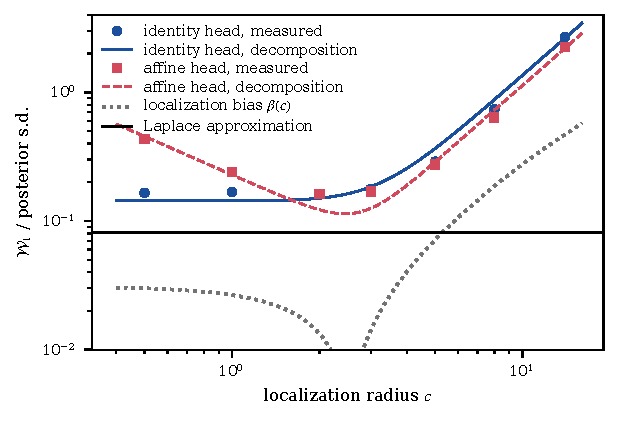
\includegraphics[width=0.9\textwidth]{mf_radius_theory}
\caption{The decomposition \eqref{m:eq:decomp} against measurement on the two dimensional Navier Stokes problem of Polson and Sokolov~\cite{polsonsokolov2026}, $D=6$, $M=1200$. Points are measured Wasserstein distances to an MCMC gold standard, in posterior standard deviations; curves are \eqref{m:eq:decomp} with $a_v$ and $b$ fitted separately for each head, and the bias $\beta(c)$ (dotted) is computed from \eqref{m:eq:bias} with no free parameter; the horizontal line is the Laplace approximation on the same run. The fitted optimum for the affine head is $c^\star=2.44$ against a measured optimum between $2$ and $3$; the root mean square residual of that fit is $0.044$. The localization bias is negligible below $c\approx3$, so in the fit of the affine head the left arm is estimation variance and the right arm nonlinearity. The identity head is the one produced by the study's script, whose residuals are neither centered at their sample mean nor rescaled, so that its flat left arm contains the displacement of Theorem~\ref{m:thm:locbias}(ii), which does not depend on $c$.}\label{m:fig:radius}
\end{figure}

Figure~\ref{m:fig:radius} tests \eqref{m:eq:decomp} on the Navier Stokes problem, with $a_v$ and $b$ fitted by least squares on the measured errors, which range from $0.16$ to $2.7$; the affine head's predicted optimum matches the measured one. The identity head's flat left arm is correctly predicted by $v=0$ (its level is mostly the displacement of Theorem~\ref{m:thm:locbias}(ii) and not the variance term), and the affine head's steep left arm by $v=2$: with a narrow proposal there is no design spread from which to estimate a slope.

\subsection{The design rule, and what it changes}

\begin{algorithm}[Localized GBC]\label{m:alg:loc}
Replace the step of Algorithm~\ref{m:alg:gbc} that simulates the training pairs by the following.
\begin{enumerate}[nosep]
\item Compute a preliminary estimate $\bar\theta_N$ and its Gauss Newton covariance $\Sigma_N$.
\item Draw $\theta^{(m)}\sim N(\bar\theta_N,c^2\Sigma_N)$ with $c\in[2,3]$, and simulate $Z^{(m)}$ from those.
\item Use the identity head with residuals centered at their sample mean (in the linear Gaussian model, equivalently, subtract $P\bar\theta_N$), and whiten by the sample covariance of the centered residuals rescaled by $(s_j+c^2p_j^2)^{-1/2}$ in the eigenbasis of $P$.
\item Do not add the residual mean to the center; do not use an affine head; do not importance weight back to the prior.
\end{enumerate}
\end{algorithm}

The radius $c\in[2,3]$ is not read off \eqref{m:eq:cstar}; the range is calibrated on the measurement, as Remark~\ref{m:rem:radiushead} sets out. Centering the residuals is Theorem~\ref{m:thm:locbias}(ii) and is the most consequential line of the algorithm; without it the generator carries a first order bias that no number of simulations removes. The rescaling is the second: without it the head reports the spread of the \emph{proposal} rather than of the posterior (Theorem~\ref{m:thm:locbias}(iii) and Remark~\ref{m:rem:rescale}). The prohibition on importance weighting is empirical and is explained by Theorem~\ref{m:thm:locbias}: the correction is unnecessary, because by Corollary~\ref{m:cor:locG}(i) there is no bias to remove once the residuals are centered and rescaled, while the weights $\pi/q_c$ are ratios of Gaussians with the wider density in the numerator and therefore have infinite variance whenever $c^2p_j\le1/2$ in some direction $j$, as in the data dominated directions here; in the Navier Stokes study the effective sample size never exceeded $34$ of $1200$ at any radius.

Algorithm~\ref{m:alg:loc} is a way of meeting (G1). Corollary~\ref{m:cor:locG} proves this in the linear Gaussian model. Localization is not new to the theory. The Bernstein von Mises theorems behind Theorem~\ref{m:thm:jwbvm} are proved on a localization set of the posterior, and Nickl and Wang~\cite{nicklwang2024}, in a steady state Schr\"odinger model, build their sampler on a surrogate log likelihood that agrees with the likelihood on a ball about a data driven initializer, of radius a small multiple of $D^{-4/d}$ with $D$ the dimension of their discretization, set by their stability estimate; only the training step had been left outside such a set.

\begin{corollary}[The localized design meets (G1) and (G2)]\label{m:cor:locG}
Consider the generator of Algorithm~\ref{m:alg:loc} with proposal $q_c=N(\bar\theta_N,c^2\Sigma_N)$ and $P=\Sigma_N\Sigma_0^{-1}$. In the setting of Lemma~\ref{m:lem:exact}, with $\Sigma_0$ and $\Phi^\top\Phi$ commuting as in Theorem~\ref{m:thm:locbias}:
\begin{enumerate}[label=(\roman*),nosep]
\item \emph{(Exactness in population.)} For every $c>0$ and every center $\bar\theta_N$, the law the head produces at the observed data is exactly the posterior, $N\big(S(Y),\Sigma_N\big)$. Localization contributes no bias at all, not merely a bias of smaller order.
\item \emph{(Finite $M$.)} With $M=M_N$ simulations and $J=J_N$ retained modes, the rescaled sample covariance of the centered residuals equals $\Sigma_N^{1/2}(\Id+\Delta_M)\Sigma_N^{1/2}$, where $\norm{\Delta_M}_{op}=O_P\big(\sqrt{J_N/M_N}+J_N/M_N\big)$ does not depend on $c$. Hence, when $\Sigma_{N,j}\lesssim\lambda_j/N$ on the retained modes ($\lambda_j$ the Laplace eigenvalues), as for the heat and Stokes equations, and $k>d/2$, $\Wone_{1,H^{-k-2}}(\Pihat,\PiN)=O_P\big(N^{-1/2}(\sqrt{J_N/M_N}+J_N/M_N)\big)$, so (G1) holds whenever $J_N/M_N\to0$, at every radius; and (G2) holds at every order whenever the exact posterior $N(S(Y),\Sigma_N)$ satisfies its first clause.
\item Consequently Theorem~\ref{m:thm:main} applies verbatim to Algorithm~\ref{m:alg:loc}, and Assumption~\ref{m:ass:G} is discharged for it.
\end{enumerate}
Part (i) does not use Assumption~\ref{m:ass:U}: in the linear Gaussian model the posterior given the summary is the posterior, so the two terms of Theorem~\ref{m:thm:qnnA} that need it vanish identically. Parts (ii) and (iii) quote the argument of Theorem~\ref{m:thm:qnnA}, and Remark~\ref{m:rem:u2pres} says what they need for a nonlinear forward map and what of it is open. Assumption~\ref{m:ass:u2p} itself is proved by Theorem~\ref{m:thm:u2ploc}, under the hypotheses there, for the uncentered and unrescaled head of Definition~\ref{m:def:gen}, so that Theorem~\ref{m:thm:qnnA} applies to that head under its other hypotheses.
\end{corollary}

\begin{proof}
(i) Write $A=\Sigma_NF$, so that $A+P=\Sigma_N(F+\Sigma_0^{-1})=\Id$, and $S=\Sigma_N\Phi^\top Y/\varsigma^2=A\theta+\Sigma_N\Phi^\top\varepsilon/\varsigma^2$. Hence
\[
R=\theta-S=P\theta-\Sigma_N\Phi^\top\varepsilon/\varsigma^2 ,
\]
which is Theorem~\ref{m:thm:locbias}: $E_{q_c}R=P\bar\theta_N$ and $\Var_{q_c}R=c^2P\Sigma_NP^\top+\Sigma_NF\Sigma_N$, equal to $\Sigma_{N,j}(s_j+c^2p_j^2)$ in the basis diagonalizing $P$. Subtracting the mean removes $P\bar\theta_N$ exactly, and dividing coordinate $j$ by $(s_j+c^2p_j^2)^{1/2}$ leaves variance exactly $\Sigma_{N,j}$; the rescaled residual is therefore $N(0,\Sigma_N)$, and the head returns $S(Y)+N(0,\Sigma_N)$, which by Lemma~\ref{m:lem:exact} is the exact posterior. What makes this work is not independence of $R$ and $S$, which fails under $q_c$: $\mathrm{Cov}_{q_c}(R,S)=(c^2P-\Id)\Sigma_NF\Sigma_N$, zero only when $c^2\Sigma_N=\Sigma_0$, as for the true prior. The head does not condition on $S$; it draws from the marginal law of the corrected residual and adds it to $S$, and that composition has the right conditional law because the corrected residual is $N(0,\Sigma_N)$ whatever $Y$ is.

(ii) Work in the basis diagonalizing $P$, $\Sigma_N$ and $F$, and let $V=\Var_{q_c}R$, diagonal with entries $\Sigma_{N,j}(s_j+c^2p_j^2)$ by (i). In the linear Gaussian model the residuals are $R^{(m)}=P\bar\theta_N+V^{1/2}g_m$ with $g_m$ i.i.d.\ $N(0,\Id_J)$, so the sample covariance of the centered residuals is $V^{1/2}(\Id+\Delta_M)V^{1/2}$, with $\Id+\Delta_M$ the sample covariance of the $g_m$; by the covariance estimation bound for Gaussian vectors~\cite[Theorem 4.7.1 and Exercise 4.7.3]{vershynin2018} with $u=J$, $\norm{\Delta_M}_{op}=O_P(\sqrt{J/M}+J/M)$, centering at the sample mean adding a term of rank one and of size $O_P(J/M)$. The rescaling is the diagonal matrix $Q$ with entries $(s_j+c^2p_j^2)^{-1/2}$, and $QV^{1/2}=\Sigma_N^{1/2}$, so the rescaled sample covariance is $\Sigma_N^{1/2}(\Id+\Delta_M)\Sigma_N^{1/2}$ and the radius drops out. The center of $\Pihat$ is $S(Y)$, as in (i), so coupling $\Pihat$ and $\PiN=N(S(Y),\Sigma_N)$ through a common $g\sim N(0,\Id_J)$ (Lemma~\ref{m:lem:coupling}) and using $|(1+x)^{1/2}-1|\le|x|$ for $x\ge-1$ gives
\[
\Wone_{1,H^{-k-2}}(\Pihat,\PiN)\le\big\|\Lambda^{-(k+2)/2}\Sigma_N^{1/2}\big\|_{HS}\,\norm{\Delta_M}_{op},
\]
where $\norm{\Lambda^{-(k+2)/2}\Sigma_N^{1/2}}^2_{HS}\le\sum_j\lambda_j^{-k-2}\Sigma_{N,j}\lesssim N^{-1}\sum_j\lambda_j^{-k-1}$ because $\Sigma_{N,j}\lesssim1/(N\iota_j)\lesssim\lambda_j/N$, and the sum is finite because $k>d/2$. For (G2), $\Pihat$ and $\PiN$ have the same center and the covariance of $\Pihat$ is at most $1+\norm{\Delta_M}_{op}$ times $\Sigma_N$, so the Gaussian concentration bounds in the proof of Theorem~\ref{m:thm:qnnA}, applied to either covariance, give spreads $O_P(r_N(s))$ in $H^s$. If $\PiN$ satisfies the first clause of (G2) with a constant $L$, then with probability above one half a draw from $\PiN$ lies in $\bar\Theta_{N,L}$, within $L\tilde\delta_N(0)$ of $S(Y)$ in $L^2$ and within $L$ of it in $H^{\bar\gamma}$, so $\norm{S(Y)-\theta_0}_{L^2}\le2L\tilde\delta_N(0)$ and $\norm{S(Y)}_{H^{\bar\gamma}}\le2L$ with probability tending to one, and the tail bound of that proof, with $L_1$ enlarged accordingly, gives (G2) for $\Pihat$ at every order.

(iii) is (i), (ii) and Theorem~\ref{m:thm:main}.
\end{proof}

\begin{remark}[Why the rescaling is not optional]\label{m:rem:rescale}
Without it the head reports $\sqrt{s_j+c^2p_j^2}$ times the correct posterior standard deviation in direction $j$, which is Theorem~\ref{m:thm:locbias}(iii). In the setting of Section~\ref{m:sec:expstudy}, $N=5\times10^4$ with $D=8$ retained modes of which $k_{\rm eff}=3$ are data dominated, the largest prior fraction is $p_{\max}=0.999$. The factor $\sqrt{1-p_j+c^2p_j^2}$ is at most one for every $p_j$ when $c=1$, so at that radius the unrescaled head \emph{understates} the posterior standard deviation, by at most $11\%$ over the eight modes, attained at $p_j=0.29$; for $c>1$ it overstates in every direction with $p_j>1/c^2$, by a factor that reaches $2.0$ at $c=2$, $3.0$ at $c=3$ and $8.0$ at $c=8$ in the most prior dominated direction.
\end{remark}

\begin{remark}[Which covariance the algorithm uses, and whether exactness survives it]\label{m:rem:whichcov}
$\Sigma_N$ in Algorithm~\ref{m:alg:loc} is $(F_{\bar\theta_N}+\Sigma_0^{-1})^{-1}$ with $F_{\bar\theta_N}$ the realized information $F_N$ of Remark~\ref{m:rem:reg}, that is the Gauss Newton information of the $N$ observations at the preliminary estimate, formed on the observed design. It is formed once and serves the proposal $c^2\Sigma_N$, the eigenbasis of $P$, and the factors $(s_j+c^2p_j^2)^{-1/2}$ alike; it is not reevaluated at the training draws, which is what keeps the cost at one Gauss Newton solve rather than $M$.

In the linear model nothing is plugged in, since $F=\Phi^\top\Phi/\varsigma^2$ does not depend on the point of evaluation; Corollary~\ref{m:cor:locG}(i) holds as stated. Nonlinearly it is a plug in and (i) does not survive verbatim. One thing does: one matrix serves both the proposal and the rescaling, so for the linearized residuals the correction $(s_j+c^2p_j^2)^{-1/2}$ undoes the inflation that produced them whatever $F_{\bar\theta_N}$ is. Two errors are left over. One is the discrepancy between $\Sigma_N(\bar\theta_N)$ and the Bernstein von Mises covariance, the same plug in error of order $\tilde\delta_N(\zeta)$ that Section~\ref{m:sec:qnn} bounds under the Lipschitz clause (U3). The other is the nonlinear remainder of the residuals under $q_c$, which Proposition~\ref{m:prop:locres} controls for a reused design. Granted the hypotheses that Remark~\ref{m:rem:u2pres} lists for parts (ii) and (iii), both enter (G1) additively alongside the $\sqrt{J_N/M_N}$ of (ii), and what is lost is the sharper reading of (i), that localization costs nothing at all rather than something of smaller order.
\end{remark}

\begin{remark}[The remaining term]\label{m:rem:relin}
In \eqref{m:eq:decomp} the term $b\,c^4$ arises because the summary is linearized once, at $\bar\theta_N$. Lemma~\ref{m:lem:exact} says that in the linear model the summary does not depend on the linearization point at all; the $c^4$ term is therefore purely a nonlinear effect, and it can be removed by iterating the Gauss Newton step and recomputing the Jacobian from the data alone at each iterate instead of once at $\bar\theta_N$, at a cost of $D+1$ forward solves per training draw for each extra step. Recomputing it at the training parameter $\theta^{(m)}$ would not define a statistic, since that parameter is not available for the observed data. The decomposition then reduces to $\beta(c)^2+a_v/c^v$, which for the affine head decreases in $c$ until the bias $\beta(c)$ begins to grow, so the optimal radius moves out to where the localization bias binds, and the achievable error is within $O(\sqrt{D/M})$ of the smallest value of $\beta(c)$, the floor it approaches as $M$ grows. Polson and Sokolov~\cite{polsonsokolov2026} carried this out with a two step Gauss Newton summary and confirmed that the $c^4$ term disappears; the error of the affine head at $c=6$ fell from $0.37$ to $0.16$ and became flat in $c$. After centering, the localized GBC posterior and the Laplace approximation agree with each other and with a $4500$ sample MCMC reference to the reference's own Monte Carlo error, $0.06$ posterior standard deviations. The cubic correction to the center, the first order shift $\frac12H^{-1}g$ of the posterior mean from the maximum a posteriori estimate, where $H$ is the negative Hessian of the log posterior density $\ell$ at the maximum and $g_a=\sum_{b,c}(H^{-1})_{bc}\,\partial_a\partial_b\partial_c\ell$ there, is at most $0.01$ standard deviations there, so the posterior is Gaussian in its center to that accuracy and neither method has anything left to correct in the well specified $T_0=0$ regime.
\end{remark}

\subsection{The whitened residuals of a localized proposal}\label{m:sec:u2ploc}

Everything is conditional on the data: $P$, $E$ and $\norm\cdot_{\psi_2}$ refer to the draw of the training pairs with $Z^{(N)}$ fixed, unless $P^\N_{\theta_0}$ is written. A simulated data set $Z^{(m)}$ is drawn from \eqref{m:eq:model} at $\theta^{(m)}$, with its own design points $X^{(m)}_i$, uniform on $\mathcal X$, and its own noise $\varepsilon^{(m)}_i\sim N(0,I_W)$, independent of each other and of $\theta^{(m)}$.

\emph{Notation.} Write $X$ for a uniform point of $\mathcal X$, $d_W$ for the dimension of an observation, $E_J=\mathrm{span}\{e_j:j\le J\}$, identified with $\R^J$, $P_J$ for the orthogonal projection onto it, $Q_J=\Id-P_J$, and $J=J_N$, so that $p_N=P_J$ in \eqref{m:eq:summary}. For a linear map $\mathcal T$ from $\ell^2$ into $\R^{d_W}$ valued functions on $\mathcal X$ let $\norm{\mathcal T}_{\ell^2\to L^2}=\sup_{\norm g_2\le1}(E\norm{(\mathcal Tg)(X)}^2_W)^{1/2}$. At a point $\vartheta$ where the linearization $\I_\vartheta$ is defined, define $K'_\vartheta$ by
\begin{equation}\label{m:eq:u2pF}
\langle f,(\Id+K'_\vartheta)g\rangle=E\big\langle(\I_\vartheta\mathcal D^{1/2}f)(X),(\I_\vartheta\mathcal D^{1/2}g)(X)\big\rangle_W ,
\end{equation}
that is $\Id+K'_\vartheta=T^{-1}\mathcal D^{1/2}\I^*_\vartheta\I_\vartheta\mathcal D^{1/2}$. Then $K'_{\theta_0}=K'$, $\norm{\I_\vartheta\mathcal D^{1/2}}^2_{\ell^2\to L^2}=\norm{\Id+K'_\vartheta}_{op}$, and $\Id+\Xi_\vartheta=P_J(\Id+K'_\vartheta)^{-1}P_J$. Fix a linearization point $\bar\vartheta$ determined by $Z^{(N)}$ at which $\Id+K'_{\bar\vartheta}$ is bounded and invertible, and let the training summary be \eqref{m:eq:summary} with one fold and the linearization point held at $\bar\vartheta$. It is linearized once, as in Remark~\ref{m:rem:relin}, but it uses the population information and carries no prior term, unlike the regularized summary of Lemma~\ref{m:lem:exact}: for $j\le J$,
\begin{equation}\label{m:eq:trainsummary}
\begin{aligned}
\hat S^{(m)}_{N,j}&=\langle e_j,\bar\vartheta\rangle\\
&\quad+\frac1N\sum_{i\le N}\Big\langle\I_{\bar\vartheta}\,p_N\big(\bar e_j^{\,\bar\vartheta}\big)(X^{(m)}_i),\;Y^{(m)}_i-u_{\bar\vartheta}(X^{(m)}_i)\Big\rangle_W .
\end{aligned}
\end{equation}
Since $\bar e_j^{\,\vartheta}=\mathcal D^{1/2}(\Id+K'_\vartheta)^{-1}\mathcal D^{1/2}e_j$ and $\mathcal D$ commutes with $P_J$, the whitened weights $\phi_j(x)=\iota_j^{1/2}\,\I_{\bar\vartheta}p_N(\bar e_j^{\,\bar\vartheta})(x)\in\R^{d_W}$ satisfy
\begin{equation}\label{m:eq:u2pW}
\sum_{j\le J}v_j\phi_j(x)=\big(\I_{\bar\vartheta}\mathcal D^{1/2}P_J(\Id+K'_{\bar\vartheta})^{-1}v\big)(x),\qquad v\in\R^J .
\end{equation}
Let $\phi(x)$ be the $J\times d_W$ matrix with rows $\phi_j(x)^\top$, so that the left side of \eqref{m:eq:u2pW} is $\phi(x)^\top v$, and write
\[
\begin{gathered}
G_\phi=E\,\phi(X)\phi(X)^\top,\qquad\hat G^{(m)}_\phi=\frac1N\sum_{i\le N}\phi(X^{(m)}_i)\phi(X^{(m)}_i)^\top,\\
b_J=\mathrm{ess\,sup}_x\norm{\phi(x)}^2_{op}
\end{gathered}
\]
for the Gram matrix of the whitened weights, its realized version and its envelope. Since $\norm{\phi\phi^\top}_F\le\norm\phi_{op}\norm\phi_F$, Chebyshev's inequality gives, for $t>0$ and the realized Gram matrix $\hat G_\phi$ of any $N$ independent uniform points of $\mathcal X$,
\begin{equation}\label{m:eq:u2pcheb}
\begin{aligned}
P\big(\norm{\hat G_\phi-G_\phi}_{op}>t\big)&\le t^{-2}E\norm{\hat G_\phi-G_\phi}^2_F\\
&\le\frac{E\norm{\phi(X)\phi(X)^\top}^2_F}{Nt^2}\le\frac{b_J\tr G_\phi}{Nt^2} .
\end{aligned}
\end{equation}
Substituting $Y^{(m)}_i=u_{\theta^{(m)}}(X^{(m)}_i)+\varepsilon^{(m)}_i$ in \eqref{m:eq:trainsummary} gives, for $v\in\R^J$,
\begin{equation}\label{m:eq:u2pdecomp}
\langle v,W^{(m)}\rangle=\mu_v-\frac1{\sqrt N}\sum_{i\le N}\big\langle\phi(X^{(m)}_i)^\top v,\varepsilon^{(m)}_i\big\rangle_W ,
\end{equation}
with $\mu_v$ a function of $Z^{(N)}$, $\theta^{(m)}$ and the design, so that conditionally on these $\langle v,W^{(m)}\rangle$ is normal with variance $v^\top\hat G^{(m)}_\phi v$.

\begin{lemma}[The Gram matrix of the whitened weights]\label{m:lem:u2pgram}
Let $\mathcal A=\Id+K'_{\bar\vartheta}$ be bounded on $\ell^2$ with $\mathcal A\succeq a\Id$ for some $a>0$, and write $B_J=\Id+\Xi_{\bar\vartheta}=P_J\mathcal A^{-1}P_J$. Then
\[
G_\phi=B_J+B_JP_J\mathcal AQ_J(Q_J\mathcal AQ_J)^{-1}Q_J\mathcal AP_JB_J ,
\]
so that $G_\phi\succeq B_J\succeq\norm{\mathcal A}^{-1}_{op}\Id$ and $\norm{G_\phi-B_J}_{op}\le a^{-3}\norm{K'_{\bar\vartheta}Q_J}^2_{op}$.
\end{lemma}

\begin{proof}
By \eqref{m:eq:u2pW} and \eqref{m:eq:u2pF}, $G_\phi=B_JP_J\mathcal AP_JB_J$ on $E_J$, and block inversion of $\mathcal A$ on $E_J\oplus Q_J\ell^2$ gives $B_J^{-1}=P_J\mathcal AP_J-P_J\mathcal AQ_J(Q_J\mathcal AQ_J)^{-1}Q_J\mathcal AP_J$; substituting gives the display, whose second term is positive semidefinite. Also $\mathcal A^{-1}\succeq\norm{\mathcal A}^{-1}_{op}\Id$, $\norm{Q_J\mathcal AP_J}_{op}=\norm{Q_JK'_{\bar\vartheta}P_J}_{op}\le\norm{K'_{\bar\vartheta}Q_J}_{op}$ by self adjointness, and $\norm{B_J}_{op}$ and $\norm{(Q_J\mathcal AQ_J)^{-1}}_{op}$ are at most $a^{-1}$.
\end{proof}

\begin{proposition}[No sub Gaussian envelope for the whole residual]\label{m:prop:u2pfalse}
Let each simulated data set have its own design, as in \eqref{m:eq:model}, let the training summary be \eqref{m:eq:trainsummary}, and let the training parameters have any law given $Z^{(N)}$. Then for every $N$, every $J$ and every unit vector $v\in\R^J$
\[
\begin{gathered}
\big\|\langle v,W^{(m)}\rangle\big\|^2_{\psi_2\mid Z^{(N)}}\ge2\,\mathrm{ess\,sup}_x\norm{\phi(x)^\top v}^2_W ,\\
\sup_{\norm u_2=1}\big\|\langle u,W^{(m)}\rangle\big\|^2_{\psi_2\mid Z^{(N)}}\ge2b_J\ge\frac{2\tr G_\phi}{d_W} .
\end{gathered}
\]
If $\Id+K'_{\bar\vartheta}$ is bounded and $\Id+K'_{\bar\vartheta}\succeq a\Id$ for some $a>0$, then $\tr G_\phi\ge J\norm{\Id+K'_{\bar\vartheta}}^{-1}_{op}$. For the heat and Stokes equations, observed from time zero as in \eqref{m:eq:model}, $G_\phi=\Id_J$ and $\norm{\langle e_J,W^{(m)}\rangle}^2_{\psi_2\mid Z^{(N)}}\ge2\norm{e_J}^2_{L^\infty}/\iota_J\ge2/\iota_J$, which grows like $\lambda_J$ by \eqref{m:eq:iota}; for the real trigonometric basis the bound is $4/\iota_J$.
\end{proposition}

\begin{proof}
Fix a unit vector $v$ and $s^2<\mathrm{ess\,sup}_x\norm{\phi(x)^\top v}^2_W$. The set $\mathcal X_s=\{x:\norm{\phi(x)^\top v}^2_W>s^2\}$ has positive measure, so with probability $P(X\in\mathcal X_s)^N>0$, whatever $\theta^{(m)}$ is, all $N$ design points lie in it, and then the conditional variance $\sigma^2=v^\top\hat G^{(m)}_\phi v$ in \eqref{m:eq:u2pdecomp} exceeds $s^2$. For $K^2<2s^2$ the exponent of $e^{x^2/K^2-(x-\mu_v)^2/(2\sigma^2)}$ then has a positive coefficient of $x^2$, so the conditional expectation of $e^{\langle v,W^{(m)}\rangle^2/K^2}$ given $Z^{(N)}$, $\theta^{(m)}$ and the design is infinite on an event of positive probability, and $\norm{\langle v,W^{(m)}\rangle}^2_{\psi_2\mid Z^{(N)}}\ge2s^2$. This is the first inequality. For the second, let $(v_k)$ be dense in the unit sphere of $\R^J$ and $c<b_J$. Each $x$ in the set $\{x:\norm{\phi(x)}^2_{op}>c\}$, which has positive measure, has $\norm{\phi(x)^\top v_k}^2_W>c$ for some $k$, so for some $k$ the set of such $x$ has positive measure, and the first inequality with $v=v_k$ gives $2c$. Next, $\norm{\phi(x)}^2_{op}\ge\norm{\phi(x)}^2_F/d_W$ and $\mathrm{ess\,sup}_x\norm{\phi(x)}^2_F\ge E\norm{\phi(X)}^2_F=\tr G_\phi$, and $\tr G_\phi\ge\tr(\Id+\Xi_{\bar\vartheta})\ge J\norm{\Id+K'_{\bar\vartheta}}^{-1}_{op}$ by Lemma~\ref{m:lem:u2pgram}. For the heat and Stokes equations $\I_\vartheta=\Lcal$ and $\Kcal=0$ in \eqref{m:eq:fredholm}, so $K'_{\bar\vartheta}=0$, $G_\phi=\Id_J$, and $\phi(t,x)^\top e_J=\iota_J^{-1/2}e^{-\nu\lambda_Jt}e_J(x)$ by \eqref{m:eq:modeinfo}, a continuous function whose squared norm has supremum $\norm{e_J}^2_{L^\infty}/\iota_J$, at $t=0$. The first inequality with $v=e_J$ gives the bound, and $\norm{e_J}^2_{L^\infty}\ge\int_\Omega\norm{e_J}^2_W=1$.
\end{proof}

For a nonlinear forward map three conditions on the linearization take the place of the explicit structure of the heat equation, and a fourth bounds its remainder. They involve a constant $a_\star>0$ and, for every $B>0$, constants $L_\star$, $C_\infty$ and $C_Q$ that may depend on $B$, and they are required for all $\vartheta,\vartheta'$ with $\norm\vartheta_{H^{\bar\gamma}},\norm{\vartheta'}_{H^{\bar\gamma}}\le B$:
\begin{enumerate}[label=(I\arabic*),nosep]
\item $\Id+K'_{\theta_0}$ is bounded on $\ell^2$, $K'_{\theta_0}$ is compact, and $\Id+K'_{\theta_0}\succeq a_\star\Id$;
\item $\norm{(\I_\vartheta-\I_{\theta_0})\mathcal D^{1/2}}_{\ell^2\to L^2}\le L_\star\norm{\vartheta-\theta_0}_{H^\zeta}$;
\item $\norm{\I_\vartheta h}_{L^\infty(\mathcal X)}\le C_\infty\norm h_{H^\zeta}$ for all $h\in H^\zeta$;
\item $\norm{u_{\vartheta'}-u_\vartheta-\I_\vartheta[\vartheta'-\vartheta]}_{L^\infty(\mathcal X)}\le C_Q\norm{\vartheta'-\vartheta}^2_{H^\zeta}$.
\end{enumerate}
Condition (I2) is a Lipschitz bound in the whitened $H^{-1}$ metric. It gives $\norm{\Xi_\vartheta-\Xi_{\theta_0}}_{op}\lesssim\norm{\vartheta-\theta_0}_{H^\zeta}$ for $\vartheta$ near $\theta_0$, uniformly in $J$, which the weight condition \eqref{m:eq:lipweight} does not, since its factor $\norm{e_j}_{H^{\kappa+2}}$ grows with $j$. Condition (I3) at $\vartheta=\theta_0$ is the second part of Condition 2D of Nickl~\cite{nicklbvm2024}. For Navier Stokes, (I1) is shown before Assumption~\ref{m:ass:u2p}, and Lemma~\ref{m:lem:nslin} proves (I2) to (I4).

\begin{theorem}[Assumption~\ref{m:ass:u2p} under a localized proposal]\label{m:thm:u2ploc}
Let $\bar\theta_N$ be a preliminary estimate as in Definition~\ref{m:def:summary}, let $J=J_N\asymp N^{d/(2\gamma+d)}$, and let the training parameters be
\[
\theta^{(m)}=\bar\theta_N+N^{-1/2}\mathcal D^{1/2}\mathcal V_N^{1/2}\xi^{(m)},
\]
where $\mathcal V_N$ is a positive semidefinite $J\times J$ matrix determined by $Z^{(N)}$ with $\norm{\mathcal V_N}_{op}=O_P(1)$, and the $\xi^{(m)}$ are i.i.d.\ standard normal on $\R^J$ given $Z^{(N)}$, conditioned on $\norm{\xi^{(m)}}^2_2\le4J$ when the forward map is nonlinear. Let the training summary be \eqref{m:eq:trainsummary} with $\bar\vartheta=\bar\theta_N$, and the generator that of Definition~\ref{m:def:gen}, uncentered and unrescaled.
\begin{enumerate}[label=(\alph*),nosep]
\item For the heat and Stokes equations, observed from time zero as in \eqref{m:eq:model}, with $\gamma>d+2$, which the hypotheses of Theorem~\ref{m:thm:qnnA} imply, Assumption~\ref{m:ass:u2p} holds with $\Xi=0$, $\varkappa_N\le4/\sqrt3$ and $W^{(m)}_{\rm g}=-1_{\mathcal B_m}N^{-1/2}\sum_i\phi(X^{(m)}_i)\varepsilon^{(m)}_i$, where $\mathcal B_m=\{\norm{\hat G^{(m)}_\phi-\Id}_{op}\le1\}$.
\item For a nonlinear forward map, Assumption~\ref{m:ass:u2p} holds under Conditions 1 and 2 of Nickl~\cite{nicklbvm2024} with the constants of Theorem~\ref{m:thm:nickl2}, $\bar\gamma<\gamma-1$, the rate hypothesis $\sqrt N\,\tilde\delta_N(0)\tilde\delta_N(\zeta)\to0$ of Proposition~\ref{m:prop:suff}, and (I1) to (I3).
\item Let $\Sigma_0$ be positive definite, $\Sigma_N=(F_{\bar\theta_N}+\Sigma_0^{-1})^{-1}$ with $F_{\bar\theta_N}$ the realized information on $J$ modes (Remark~\ref{m:rem:whichcov}), and $a_\star=1$ in (a). Under the hypotheses of (a) or (b), with probability tending to one $N^{-1}\mathcal D^{1/2}F_{\bar\theta_N}\mathcal D^{1/2}\succeq(a_\star/12)\Id$, and then $\mathcal V_N=c^2N\mathcal D^{-1/2}\Sigma_N\mathcal D^{-1/2}$ has $\norm{\mathcal V_N}_{op}\le12c^2/a_\star$.
\end{enumerate}
\end{theorem}

The proposal $N(\bar\theta_N,c^2\Sigma_N)$ of Algorithm~\ref{m:alg:loc} on $D=J$ modes has this form with $\mathcal V_N=c^2N\mathcal D^{-1/2}\Sigma_N\mathcal D^{-1/2}$, and part (c) gives $\norm{\mathcal V_N}_{op}=O_P(1)$. For the heat and Stokes equations $N^{-1}\mathcal D^{1/2}F_{\bar\theta_N}\mathcal D^{1/2}$ is the realized Gram matrix $\hat G_\phi$ of the observed design, which tends to $\Id$ by \eqref{m:eq:u2pcheb}, since $b_JJ/N\to0$ (Step 5 below). Since $P(\norm\xi^2_2>4J)\le(4e^{-3})^{J/2}$, truncated and untruncated draws coincide except on an event of probability at most $M(4e^{-3})^{J/2}$, which tends to zero when $\log M_N=o(J_N)$. If instead the simulated data sets reuse the observed design $(X_i)_{i\le N}$ and draw only fresh noise, as in Lemma~\ref{m:lem:exact}, then for the heat and Stokes equations the computation of Step 1 below gives $W^{(m)}=-(\hat G_\phi-\Id)\mathcal V_N^{1/2}\xi^{(m)}-N^{-1/2}\sum_i\phi(X_i)\varepsilon^{(m)}_i$, which is centered Gaussian given $Z^{(N)}$ with covariance $(\hat G_\phi-\Id)\mathcal V_N(\hat G_\phi-\Id)+\hat G_\phi$. Since $\hat G_\phi\to\Id$, Assumption~\ref{m:ass:u2p} then holds with $W^{(m)}_{\rm r}=0$, and the whole residual has a sub Gaussian norm bounded uniformly in $J$ with probability tending to one.

\begin{proof}
In (a) the bounds below depend on $Z^{(N)}$ only through $\norm{\mathcal V_N}_{op}$. In (b) the events $A_N$ on which $\norm{\mathcal V_N}_{op}\le c_{\mathcal V}$, $\norm{\bar\theta_N}_{H^{\bar\gamma}}\le B$, $\norm{\bar\theta_N-\theta_0}_{H^\zeta}\le L\tilde\delta_N(\zeta)$ and $\norm{\bar\theta_N-\theta_0}_{L^2}\le L\tilde\delta_N(0)$ have probability tending to one as $c_{\mathcal V},B,L\to\infty$, uniformly in large $N$, by Definition~\ref{m:def:summary}. Let $\eta_N$ be the sum of the two quantities in the second display of Assumption~\ref{m:ass:u2p}. It suffices to show that for fixed constants, with $Z^{(N)}$ fixed, $\norm{\mathcal V_N}_{op}\le c_{\mathcal V}$ in (a) and $A_N$ in force in (b), $\varkappa_N$ is bounded and $\eta_N$ is at most a deterministic sequence that tends to zero. We drop the index $m$.

\emph{Step 1: decomposition.} Write $\mathcal A=\Id+K'_{\bar\theta_N}$, $\mathcal A_0=\Id+K'_{\theta_0}$, $\tilde h=\mathcal V_N^{1/2}\xi\in E_J$, $h=\theta-\bar\theta_N=N^{-1/2}\mathcal D^{1/2}\tilde h$ and $\tilde u=\I_{\theta_0}\mathcal D^{1/2}\tilde h$. With $R_0(\vartheta)=u_\vartheta-u_{\theta_0}-\I_{\theta_0}[\vartheta-\theta_0]$ we have $u_\theta-u_{\bar\theta_N}=N^{-1/2}\tilde u+r_\theta$, where $r_\theta=R_0(\theta)-R_0(\bar\theta_N)$ vanishes for a linear map, and substituting $Y_i=u_\theta(X_i)+\varepsilon_i$ in \eqref{m:eq:trainsummary} gives
\[
\begin{aligned}
W&=\tilde h-\frac1N\sum_i\phi(X_i)\tilde u(X_i)\\
&\quad-\frac1{\sqrt N}\sum_i\phi(X_i)r_\theta(X_i)-\frac1{\sqrt N}\sum_i\phi(X_i)\varepsilon_i .
\end{aligned}
\]
By \eqref{m:eq:u2pW}, the summands of the first sum have mean $P_J\mathcal A^{-1}P_JT^{-1}\mathcal D^{1/2}\I^*_{\bar\theta_N}\I_{\theta_0}\mathcal D^{1/2}\tilde h$ over $X$, and writing $\tilde h=P_J\mathcal A^{-1}\mathcal A\tilde h$ with $Q_J\mathcal A\tilde h=Q_JK'_{\bar\theta_N}\tilde h$ shows that $\tilde h$ minus this mean is $\mathcal C\tilde h$, where
\[
\mathcal C=P_J\mathcal A^{-1}Q_JK'_{\bar\theta_N}P_J+P_J\mathcal A^{-1}P_JT^{-1}\mathcal D^{1/2}\I^*_{\bar\theta_N}\big(\I_{\bar\theta_N}-\I_{\theta_0}\big)\mathcal D^{1/2}P_J .
\]
With the design event $\mathcal B=\{\norm{\hat G_\phi-G_\phi}_{op}\le1\}$ set
\[
\begin{aligned}
W_{\rm g}&=\mathcal C\tilde h-1_{\mathcal B}\frac1{\sqrt N}\sum_i\phi(X_i)\varepsilon_i ,\\
W_{\rm r}&=-1_{\mathcal B^c}\frac1{\sqrt N}\sum_i\phi(X_i)\varepsilon_i-\Big(\frac1N\sum_i\phi(X_i)\tilde u(X_i)-E\,\phi(X)\tilde u(X)\Big)\\
&\quad-\frac1{\sqrt N}\sum_i\phi(X_i)r_\theta(X_i),
\end{aligned}
\]
the expectation in the middle term taken over $X$ with $\tilde h$ fixed. Then $W=W_{\rm g}+W_{\rm r}$, the pairs $(W_{\rm g},W_{\rm r})$ are i.i.d.\ over the simulations given $Z^{(N)}$, and $E\,W_{\rm g}=0$, because $\xi$ is symmetric and the noise is centered and independent of $\xi$ and of the design.

\emph{Step 2: the sub Gaussian part.} Given the design and $\xi$, the variable $1_{\mathcal B}N^{-1/2}\sum_i\langle\phi(X_i)^\top v,\varepsilon_i\rangle_W$ is centered normal with variance at most $s^2=\norm{G_\phi}_{op}+1$ for unit $v$, and a centered normal variable $\chi$ with variance at most $s^2$ has $E\,e^{\chi^2/K^2}\le(1-2s^2/K^2)^{-1/2}=2$ at $K^2=8s^2/3$, so its sub Gaussian norm is at most $(8/3)^{1/2}s$. For the other term, $\langle v,\mathcal C\tilde h\rangle=\langle\mathcal V_N^{1/2}\mathcal C^\top v,\xi\rangle$, and every $\langle u,\xi\rangle$ with $\norm u_2=1$ has sub Gaussian norm at most $2\sqrt3$: $E\,e^{\langle u,\xi\rangle^2/12}=(5/6)^{-1/2}$ for the standard normal law, and conditioning on $\{\norm\xi^2_2\le4J\}$, an event of probability at least $1-(4e^{-3})^{J/2}\ge0.55$ by the Chernoff bound $P(\norm\xi^2_2\ge4J)\le e^{-3J/2}E\,e^{3\norm\xi^2_2/8}$, raises this to at most $(5/6)^{-1/2}/0.55<2$. Hence
\[
\varkappa_N\le(8/3)^{1/2}\big(\norm{G_\phi}_{op}+1\big)^{1/2}+2\sqrt3\,c_{\mathcal V}^{1/2}\norm{\mathcal C}_{op} .
\]

\emph{Step 3: the second moment.} The two terms of $W_{\rm g}$ are uncorrelated, since the second is centered given $\xi$ and the design, and $E\,\xi\xi^\top\preceq\Id$, since the truncation preserves rotation invariance and does not raise $E\norm\xi^2_2$. Hence $E\,W_{\rm g}W_{\rm g}^\top=E\,\mathcal C\tilde h\tilde h^\top\mathcal C^\top+G_\phi-E\,\hat G_\phi1_{\mathcal B^c}$, where the first term has norm at most $c_{\mathcal V}\norm{\mathcal C}^2_{op}$ and the last at most $b_JP(\mathcal B^c)\le b_J^2\tr G_\phi/N$ by \eqref{m:eq:u2pcheb}. With Lemma~\ref{m:lem:u2pgram}, $a$ a lower bound for $\mathcal A$, and $\norm{\Xi_{\bar\theta_N}-\Xi_{\theta_0}}_{op}\le\norm{\mathcal A^{-1}-\mathcal A_0^{-1}}_{op}$, this gives
\[
\begin{aligned}
\big\|E\,W_{\rm g}W_{\rm g}^\top-(\Id+\Xi)\big\|_{op}&\le c_{\mathcal V}\norm{\mathcal C}^2_{op}+\frac{b_J^2\tr G_\phi}N\\
&\quad+\frac{\norm{K'_{\bar\theta_N}Q_J}^2_{op}}{a^3}+\norm{\mathcal A^{-1}-\mathcal A_0^{-1}}_{op} .
\end{aligned}
\]

\emph{Step 4: the remainder.} Given the design, the first term of $W_{\rm r}$ has second moment $1_{\mathcal B^c}\tr\hat G_\phi\le1_{\mathcal B^c}d_Wb_J$. Given $\xi$, the middle term is an average of $N$ i.i.d.\ centered vectors, with second moment at most $N^{-1}E\norm{\phi(X)}^2_{op}\norm{\tilde u(X)}^2_W\le N^{-1}b_J\langle\tilde h,\mathcal A_0\tilde h\rangle$. Given $\theta$, the last term has second moment at most $E\norm{\phi(X)r_\theta(X)}^2_2+N\norm{E\,\phi(X)r_\theta(X)}^2_2\le(b_J+N\norm{G_\phi}_{op})E\norm{r_\theta(X)}^2_W$, because $\norm{E\,\phi r_\theta}_2=\sup_{\norm v_2=1}E\langle\phi^\top v,r_\theta\rangle_W\le\norm{G_\phi}^{1/2}_{op}(E\norm{r_\theta}^2_W)^{1/2}$. With \eqref{m:eq:u2pcheb} and $E\norm{\tilde h}^2_2\le c_{\mathcal V}J$ this gives
\[
\begin{aligned}
E\norm{W_{\rm r}}^2_2&\le\frac{3d_Wb_J^2\tr G_\phi}N+\frac{3c_{\mathcal V}b_J\norm{\mathcal A_0}_{op}J}N\\
&\quad+3\big(b_J+N\norm{G_\phi}_{op}\big)\sup_\theta E\norm{r_\theta(X)}^2_W ,
\end{aligned}
\]
the supremum taken over the support of the proposal.

\emph{Step 5: the heat and Stokes equations.} Here $K'_\vartheta=0$, $\I_\vartheta=\Lcal$ and $r_\theta=0$, so $\mathcal C=0$, $\mathcal A=\mathcal A_0=G_\phi=\Id$, $\Xi=0$ and $\varkappa_N\le(16/3)^{1/2}=4/\sqrt3$. The weights are $\phi_j(t,x)=\iota_j^{-1/2}e^{-\nu\lambda_jt}e_j(x)$ with $\norm{e_j(x)}^2_W\le2$, and $\iota_j^{-1}\le1+2\nu\lambda_jT$ by \eqref{m:eq:iota} at $T_0=0$, so $b_J\le2\sum_{j\le J}\iota_j^{-1}\lesssim J\lambda_J\asymp J^{1+2/d}$. Steps 3 and 4 bound $\eta_N$ by a constant times $b_J^2J/N\lesssim N^{(3d+4)/(2\gamma+d)-1}$, which tends to zero because $\gamma>d+2$. The hypotheses of Theorem~\ref{m:thm:qnnA} give $\gamma>3\zeta+3d/2+2$ with $\zeta>d/2$, hence $\gamma>3d+2$. This proves (a).

\emph{Step 6: a nonlinear map.} By (I2), $\upsilon_N=\norm{(\I_{\bar\theta_N}-\I_{\theta_0})\mathcal D^{1/2}}_{\ell^2\to L^2}\le L_\star L\tilde\delta_N(\zeta)\to0$. Since $\mathcal A-\mathcal A_0$ is the difference of the forms \eqref{m:eq:u2pF} at $\bar\theta_N$ and at $\theta_0$, $\norm{\mathcal A-\mathcal A_0}_{op}\le\upsilon_N(2\norm{\mathcal A_0}^{1/2}_{op}+\upsilon_N)\to0$, so for $N$ large $\mathcal A\succeq(a_\star/2)\Id$, $\norm{\mathcal A^{-1}-\mathcal A_0^{-1}}_{op}\le2a_\star^{-2}\norm{\mathcal A-\mathcal A_0}_{op}\to0$, and $\norm{K'_{\bar\theta_N}Q_J}_{op}\le\norm{K'_{\theta_0}Q_J}_{op}+\norm{\mathcal A-\mathcal A_0}_{op}\to0$, the first term because $K'_{\theta_0}$ is compact and self adjoint by (I1). Since $P_J\mathcal A^{-1}Q_J=-P_J\mathcal A^{-1}K'_{\bar\theta_N}Q_J$,
\[
\norm{\mathcal C}_{op}\le\frac2{a_\star}\Big(\norm{K'_{\bar\theta_N}Q_J}^2_{op}+\norm{\mathcal A}^{1/2}_{op}\,\upsilon_N\Big)\to0 ,
\]
while $\norm{G_\phi}_{op}\le2/a_\star+8a_\star^{-3}\norm{K'_{\bar\theta_N}Q_J}^2_{op}$ stays bounded by Lemma~\ref{m:lem:u2pgram}, so $\varkappa_N$ is bounded. By (I3) and \eqref{m:eq:u2pW}, $\norm{\phi(x)^\top v}_W\le C_\infty\norm{\mathcal D^{1/2}P_J\mathcal A^{-1}v}_{H^\zeta}\le C_\infty(2/a_\star)\max_{j\le J}(1+\lambda_j)^{\zeta/2}\iota_j^{-1/2}\norm v_2$, so $b_J\lesssim\lambda_J^{\zeta+1}$ and $b_J^2J/N\lesssim N^{(4\zeta+4+d)/(2\gamma+d)-1}\to0$, because $\gamma>3\zeta+3d/2+2>2\zeta+2$ by the hypotheses of Theorem~\ref{m:thm:nickl2}. It remains to bound $r_\theta$. On the support of the proposal, for $s\ge0$,
\[
\norm h^2_{H^s}\le\frac{4c_{\mathcal V}J}N\max_{j\le J}(1+\lambda_j)^s\iota_j^{-1}\lesssim\frac{J\lambda_J^{s+1}}N ,
\]
which tends to zero for $s=\bar\gamma$ because $\bar\gamma<\gamma-1$. So for $N$ large both $\theta-\theta_0$ and $\bar\theta_N-\theta_0$ lie in $U(\bar\gamma,B+\norm{\theta_0}_{H^{\bar\gamma}}+1)$, and Condition 2C, applied to each of the two terms of $r_\theta$, gives
\[
\big(E\norm{r_\theta(X)}^2_W\big)^{1/2}\lesssim\norm{\theta-\theta_0}^2_{L^2}+\norm{\bar\theta_N-\theta_0}^2_{L^2}\lesssim\tilde\delta_N(0)^2+\frac{J\lambda_J}N .
\]
Since $\tilde\delta_N(0)\le\tilde\delta_N(\zeta)$, the rate hypothesis gives $N\tilde\delta_N(0)^4\to0$, and $N(J\lambda_J/N)^2\asymp N^{(2d+4)/(2\gamma+d)-1}\to0$ because $\gamma>2+d/2$; also $b_J\lesssim N$. Steps 2 to 4 now give (b).

\emph{Step 7: part (c).} Let $\bar\theta_N$ be computed from $Z^{[b]}$, let $n\ge N/3$ be the size of the other half $\mathcal I_{3-b}$, and let $\psi(x)$ be the $J\times d_W$ matrix with rows $\iota_j^{-1/2}(\I_{\bar\theta_N}e_j)(x)^\top$, so that $N^{-1}\mathcal D^{1/2}F_{\bar\theta_N}\mathcal D^{1/2}\succeq(n/N)\hat G_\psi$ with $\hat G_\psi=n^{-1}\sum_{i\in\mathcal I_{3-b}}\psi(X_i)\psi(X_i)^\top$. Given $Z^{[b]}$ these $X_i$ are independent and uniform, and $E\,\psi(X)\psi(X)^\top=P_J\mathcal AP_J\succeq(a_\star/2)\Id$ by \eqref{m:eq:u2pF}, with $\mathcal A=\Id$ in (a) and, in (b), by Step 6 on the part of $A_N$ that concerns $\bar\theta_N$ and for $N$ large, where also $\norm{\mathcal A}_{op}\le\norm{\mathcal A_0}_{op}+1$. By Step 5 in (a) and by (I3) in (b), $b_\psi=\mathrm{ess\,sup}_x\norm{\psi(x)}^2_{op}$ is $O(J\lambda_J)$ and $O(\lambda_J^{\zeta+1})$, so \eqref{m:eq:u2pcheb} for $\psi$ with $t=a_\star/4$ bounds the probability that $\hat G_\psi\not\succeq(a_\star/4)\Id$ by $16b_\psi J\norm{\mathcal A}_{op}/(a_\star^2n)$, which tends to zero as in Steps 5 and 6. As $n/N\ge1/3$ and $\Sigma_N\preceq F_{\bar\theta_N}^{-1}$, (c) follows.
\end{proof}

\begin{lemma}[The linearization of the reaction diffusion class]\label{m:lem:rdlin}
In the setting of Theorem~\ref{m:thm:nickl1}, with $\theta_0\in C^\infty$, $K_f=\sup|f'|$ and $\I_\vartheta h$ the solution $U$ of $\partial_tU=\Delta U+f'(u_\vartheta)U$, $U(0)=h$, conditions (I1) to (I4) hold for every $\zeta>d/2$ and every $\bar\gamma>\max(1,\zeta)$, and $\norm{\Id+K'_\vartheta}_{op}$ is bounded by a constant that depends only on $K_f$ and $T$.
\end{lemma}

\begin{proof}
Write $\norm\cdot$ for the norm of $L^2(\Omega)$, $\norm g^2_{-1}=\langle(\Id-\Delta)^{-1}g,g\rangle$, which is the norm of $H^{-1}$ in the convention (13) of Nickl~\cite{nicklbvm2024}, and $V=f'(u_\vartheta)$, so that $|V|\le K_f$. By \eqref{m:eq:iota} with $\nu=1$ and $T_0=0$, $\iota_j(1+\lambda_j)$ lies between two positive constants that depend only on $T$, so $\norm{\mathcal D^{-1/2}g}_2$ and $\norm g_{-1}$ are equivalent norms, and since $|\Omega|=1$, $E\norm{(\I_\vartheta h)(X)}^2=T^{-1}\int_0^T\norm{\I_\vartheta h(t)}^2dt$. We prove the bounds for $h\in H^1$, for which the weak solutions of (108) of Nickl~\cite{nicklbvm2024} exist with $U\in L^2([0,T],H^1)$ and $\partial_tU\in L^2([0,T],H^{-1})$, and extend them by density.

\emph{Upper bound.} Testing (108) there with $(\Id-\Delta)^{-1}U(t)$ and using $\norm{(\Id-\Delta)^{-1}U}\le\norm U_{-1}$,
\[
\begin{aligned}
\tfrac12\tfrac d{dt}\norm U^2_{-1}&=-\norm U^2+\norm U^2_{-1}+\langle VU,(\Id-\Delta)^{-1}U\rangle\\
&\le-\tfrac12\norm U^2+\big(1+\tfrac12K_f^2\big)\norm U^2_{-1} .
\end{aligned}
\]
Gr\"onwall's inequality gives $\norm{U(t)}^2_{-1}\le e^{(2+K_f^2)t}\norm h^2_{-1}$, and integrating the inequality over $[0,T]$ then gives $\int_0^T\norm{U(t)}^2dt\le e^{(2+K_f^2)T}\norm h^2_{-1}$, a bound that does not depend on $\vartheta$.

\emph{Compactness.} Let $\mathcal Z$ be the Duhamel operator $(\mathcal Zw)(t)=\int_0^te^{(t-s)\Delta}w(s)\,ds$ on $L^2([0,T],L^2(\Omega))$. On the coefficient of $e_j$ it is convolution in time with $e^{-\lambda_jr}1_{r>0}$, a compact operator on $L^2[0,T]$ of norm at most $\min(T,\lambda_j^{-1})$ by Young's inequality, so $\mathcal Z$ is the limit in operator norm of its compact truncations to finitely many modes, and is compact. The weak solution is the mild solution $U=\Lcal h+\mathcal Z(VU)$, so $\I_\vartheta\mathcal D^{1/2}=\Lcal\mathcal D^{1/2}+\mathcal Z\,V\,\I_\vartheta\mathcal D^{1/2}$ with the second operator compact. Since $\Lcal\mathcal D^{1/2}$ is an isometry from $\ell^2$ into $L^2$ of the uniform probability on $\mathcal X$, by \eqref{m:eq:modeinfo}, expanding \eqref{m:eq:u2pF} shows that $K'_\vartheta$ is compact.

\emph{Lower bound at $\theta_0$.} The potential $f'(u_{\theta_0})$ lies in $C^1([0,T],C^1)$ for smooth $\theta_0$, by Proposition~4 of Nickl~\cite{nicklbvm2024}, and Lemma~4 there gives $\int_0^T\norm{U(s)}^2ds\ge c\norm h^2_{H^{-1}}$ for $h\in H^1$, where $\norm h_{H^{-1}}$ is bounded below by a constant times $\norm h_{-1}$, since the dual norms (16) there are equivalent to the norms (13) there for negative exponents. With the upper bound and density this gives $\Id+K'_{\theta_0}\succeq a_\star\Id$ for some $a_\star>0$, and (I1) holds.

\emph{(I2).} Let $U=\I_\vartheta h$, $U_0=\I_{\theta_0}h$, $V_0=f'(u_{\theta_0})$ and $\delta U=U-U_0$, which solves $\partial_t\delta U=\Delta\delta U+V\delta U+(V-V_0)U_0$, $\delta U(0)=0$. Testing with $\delta U$ gives $\tfrac d{dt}\norm{\delta U}^2\le(2K_f+1)\norm{\delta U}^2+\norm{V-V_0}^2_{L^\infty(\mathcal X)}\norm{U_0}^2$, and Gr\"onwall's inequality with the upper bound gives
\[
\int_0^T\norm{\delta U(t)}^2dt\le Te^{(2K_f+1)T}e^{(2+K_f^2)T}\norm{V-V_0}^2_{L^\infty(\mathcal X)}\norm h^2_{-1} .
\]
By the mean value theorem and (103) of Nickl~\cite{nicklbvm2024}, $\norm{V-V_0}_{L^\infty(\mathcal X)}\le\sup|f''|\sup_{0<t<T}\norm{u_\vartheta(t)-u_{\theta_0}(t)}_\infty\lesssim\norm{\vartheta-\theta_0}_{H^\zeta}$, with a constant that depends on $f$ and on a bound for $\norm\vartheta_{H^\zeta}+\norm{\theta_0}_{H^\zeta}$, which $\norm\vartheta_{H^{\bar\gamma}}\le B$ supplies because $\bar\gamma>\zeta$. With $h=\mathcal D^{1/2}g$ this is (I2).

\emph{(I3).} Write $\mathcal Z_Vw=\mathcal Z(Vw)$, so that the mild solution is the series $U=\sum_{n\ge0}\mathcal Z_V^n\Lcal h$. The heat semigroup is positive and satisfies $e^{(t-s)\Delta}e^{s\Delta}=e^{t\Delta}$, so induction gives $|(\mathcal Z_V^n\Lcal h)(t)|\le(K_ft)^n(n!)^{-1}e^{t\Delta}|h|$ pointwise. The series therefore converges uniformly on $\mathcal X$, its sum is the mild solution, which is unique because the powers $\mathcal Z_V^n$ have norms at most $(K_fT)^n/n!$, and $|U(t,x)|\le e^{K_fT}\norm h_\infty$. Finally, since $\norm{e_j}_\infty\le\sqrt2$, $\norm h_\infty\le\sqrt2\sum_j|\langle h,e_j\rangle|\le\big(2\sum_j(1+\lambda_j)^{-\zeta}\big)^{1/2}\norm h_{H^\zeta}$, finite for $\zeta>d/2$.

\emph{(I4).} With $w=u_{\vartheta'}-u_\vartheta$ and $V=f'(u_\vartheta)$, the mild form of the equations gives $z=w-\I_\vartheta[\vartheta'-\vartheta]$ as $z(t)=\int_0^te^{(t-s)\Delta}(Vz+q)(s)\,ds$, where $|q|=|f(u_{\vartheta'})-f(u_\vartheta)-Vw|\le\frac12\sup|f''|\,w^2$. The heat semigroup does not increase the supremum norm, and $z$ is bounded by (103) of Nickl~\cite{nicklbvm2024} and (I3), so Gr\"onwall's inequality and (103) give $\norm z_{L^\infty(\mathcal X)}\lesssim\sup_t\norm{w(t)}^2_\infty\lesssim\norm{\vartheta'-\vartheta}^2_{H^\zeta}$.
\end{proof}

\begin{lemma}[The linearization of the Navier Stokes equations]\label{m:lem:nslin}
For the Navier Stokes equations of Section~\ref{m:sec:ns} with $f\in\Hds{1}$ and $\theta_0\in\Hds{2}$, conditions (I2) to (I4) hold with $\zeta=2$ for every $\bar\gamma\ge2$. If moreover $f,\theta_0\in\Hds{\infty}$, as in Theorem~2.11 of Konen and Nickl~\cite{konennickl2026}, then with (I1), and with Condition 2C from their Proposition~3.8(iii), every hypothesis of Theorem~\ref{m:thm:u2ploc}(b) on the forward map holds, with their Condition 2.12 in place of Condition 2 and $\gamma=\alpha>12>3\zeta+3d/2+2$.
\end{lemma}

\begin{proof}
We use the homogeneous norms of Konen and Nickl~\cite{konennickl2026}, with $\norm\cdot_{\Hds{a}}\le\norm\cdot_{H^a}$ for $a\ge0$, and their Propositions~3.4, 3.7, 3.9, 3.12 and~4.1 with $a\in\{-1,2\}$, where $a^*=2$; the constants depend on $\nu$, $T$, $\norm f_{\Hds{1}}$ and $L=2(B+\norm{\theta_0}_{\Hds{2}})$, which bounds the $\Hds{2}$ norms of the initial conditions. For $h\in\Hds{1}$, by their Proposition~3.8(ii), $\delta U=\I_\vartheta[h]-\I_{\theta_0}[h]$ solves their equation (4.4) with $\theta=\theta'=\vartheta$, $\xi=0$ and $g=-B[w,U_0]-B[U_0,w]$, where $w=u_\vartheta-u_{\theta_0}$ and $U_0=\I_{\theta_0}[h]$, and, lying in $C([0,T],\Hds{1})\cap L^2([0,T],\Hds{2})$ by their Proposition~3.9 with $a=1$, it is the unique solution of their Proposition~4.1 with $a=-1$, which gives the first inequality in $\int_0^T\norm{\delta U}^2_{L^2}dt\lesssim\int_0^T\norm g^2_{\Hds{-2}}dt\lesssim\norm{\vartheta-\theta_0}^2_{\Hds{2}}\norm h^2_{\Hds{-1}}$, and their Proposition~3.4 with $a=-1$, the Poincar\'e inequality and their Propositions~3.7 with $a=2$ and~3.9 with $a=-1$ give the second. The bound extends to $h\in\Hds{-1}$ by density, and since $E\norm{\delta U(X)}^2=T^{-1}\int_0^T\norm{\delta U}^2_{L^2}dt$ and $\norm{\mathcal D^{1/2}v}^2_{\Hds{-1}}=\sum_jv_j^2/(\lambda_j\iota_j)\le2\nu T\norm v^2_2/(1-e^{-2\nu\lambda_1T})$ by \eqref{m:eq:iota}, it is (I2). Their Propositions~3.9 and~3.12 with $a=2$ bound $\sup_t\norm{\I_\vartheta[h](t)}_{\Hds{2}}$ by a multiple of $\norm h_{\Hds{2}}$, and $\sup_t\norm{u_{\vartheta'}(t)-u_\vartheta(t)-\I_\vartheta[\vartheta'-\vartheta](t)}_{\Hds{2}}$ by a multiple of $\norm{\vartheta'-\vartheta}^2_{\Hds{2}}$, and $\Hds{2}\subset C(\Omega)^2$ gives (I3) and (I4).
\end{proof}

\begin{remark}[The centered and rescaled residuals of Algorithm~\ref{m:alg:loc}]\label{m:rem:u2pres}
Theorem~\ref{m:thm:u2ploc} concerns the head of Definition~\ref{m:def:gen} with the summary \eqref{m:eq:trainsummary}. That head needs neither correction of step~3 of Algorithm~\ref{m:alg:loc}: $E\,W^{(m)}=E\,W^{(m)}_{\rm r}$ tends to zero, and $E[W^{(m)}W^{(m)\top}\mid Z^{(N)}]$ tends to $\Id+\Xi$ at every fixed radius, since Theorem~\ref{m:thm:u2ploc} holds for every $\mathcal V_N$ with $\norm{\mathcal V_N}_{op}=O_P(1)$ and the radius enters only through $\mathcal V_N$. The corrections belong to the regularized summary of Lemma~\ref{m:lem:exact}, and for its centered and rescaled residuals Assumption~\ref{m:ass:u2p} is not the right hypothesis. In the setting of Corollary~\ref{m:cor:locG} for the heat and Stokes equations, where $\Xi=0$, the centered and rescaled residual is exactly $N(0,\Sigma_N)$ by part (i) there, so its whitened second moment matrix is $N\mathcal D^{-1/2}\Sigma_N\mathcal D^{-1/2}$, whose $J$th diagonal entry is at most $N\iota_J\sigma^2_{0,J}$, with $\sigma^2_{0,J}=\lambda_J^{-\gamma}/(N\delta_N^2)$ the prior variance in \eqref{m:eq:prior}. Since $\iota_J\lesssim\lambda_J^{-1}$, that entry is at most of order $\lambda_{J_N}^{-\gamma-1}\delta_N^{-2}\asymp N^{-2/(2\gamma+d)}$, so the matrix stays at distance nearly one from $\Id$ in operator norm although the law is exact. Corollary~\ref{m:cor:locG}(ii) proves (G1) for that head by comparison with $N(S(Y),\Sigma_N)$ rather than with $N(\hat S_N,\Sigma/N)$. For a nonlinear forward map, parts (ii) and (iii) of that corollary inherit the hypotheses of Theorem~\ref{m:thm:qnnA}, Assumption~\ref{m:ass:U} and the hypothesis on the summary included, and need in place of Assumption~\ref{m:ass:u2p} an analogue for the centered and rescaled residuals under $q_c$ and a comparison of $N(S(Y),\Sigma_N)$ with $\PiN$. Proposition~\ref{m:prop:locres} proves that analogue when the observed design is reused; the rest is open, and parts (ii) and (iii) are not proved for a nonlinear forward map.
\end{remark}

\begin{proposition}[The centered and rescaled residuals for a nonlinear forward map]\label{m:prop:locres}
Let $\Sigma_N$ be as in Theorem~\ref{m:thm:u2ploc}(c), $c>0$ and $\theta^{(m)}=\bar\theta_N+c\Sigma_N^{1/2}\xi^{(m)}$, with $\xi^{(m)}$ as in Theorem~\ref{m:thm:u2ploc}. Let the simulated data sets reuse the observed design, let $S^{(m)}$ be their regularized summaries \eqref{m:eq:regsummary} on $J$ modes, formed at $\bar\theta_N$ with this $\Sigma_N$, and let $Q$ be the rescaling of Algorithm~\ref{m:alg:loc}. Then $\Sigma_N^{-1/2}Q(P_J\theta^{(m)}-S^{(m)})=\mu_N+W^{(m)}_{\rm g}+W^{(m)}_{\rm r}$ with $\mu_N$ determined by $Z^{(N)}$, and under the hypotheses of Theorem~\ref{m:thm:u2ploc}(b) and (I4) the pairs $(W^{(m)}_{\rm g},W^{(m)}_{\rm r})$ satisfy Assumption~\ref{m:ass:u2p} with $\Id$ in place of $\Id+\Xi$, and $\max_m\norm{W^{(m)}_{\rm r}}_2\to0$ in probability. If $J_N/M_N\to0$, the head of Algorithm~\ref{m:alg:loc}, centered at $S(Y)$, satisfies $\sqrt N\,\Wone_{1,H^{-k-2}}(\Pihat,N(S(Y),\Sigma_N))\to0$ in probability.
\end{proposition}

\begin{proof}
Write $F=F_{\bar\theta_N}=\Phi^\top\Phi$, with $\Phi$ the values of $\I_{\bar\theta_N}e_1,\dots,\I_{\bar\theta_N}e_J$ at the observed design, $\tilde\Phi=\Phi\Sigma_N^{1/2}$ and $\tilde P=\Sigma_N^{1/2}\Sigma_0^{-1}\Sigma_N^{1/2}=\Id-\tilde\Phi^\top\tilde\Phi$. Then $0\preceq\tilde P\preceq\Id$ and $P=\Sigma_N^{1/2}\tilde P\Sigma_N^{-1/2}$, so $Q=\Sigma_N^{1/2}\tilde Q\Sigma_N^{-1/2}$ with $\tilde Q=(\Id-\tilde P+c^2\tilde P^2)^{-1/2}$. Drop the index $m$, let $h=\theta-\bar\theta_N$ and let $\varrho$ be the values at the design of $u_\theta-u_{\bar\theta_N}-\I_{\bar\theta_N}h$. The simulated residuals are $\Phi h+\varrho+\varepsilon$, and the cancellation in the proof of Lemma~\ref{m:lem:exact}, which uses only $\Sigma_N(F+\Sigma_0^{-1})=\Id$, gives $P_J\theta-S=PP_J\theta-\Sigma_N\Phi^\top(\varepsilon+\varrho)$, so $\Sigma_N^{-1/2}Q(P_J\theta-S)=\mu_N+W_{\rm g}+W_{\rm r}$ with $\mu_N=\tilde Q\tilde P\Sigma_N^{-1/2}P_J\bar\theta_N$, $W_{\rm g}=\tilde Q(c\tilde P\xi-\tilde\Phi^\top\varepsilon)$ and $W_{\rm r}=-\tilde Q\tilde\Phi^\top\varrho$. As $c^2p^2$ and $1-p$ are at most $1-p+c^2p^2$ on $[0,1]$, $\norm{c\tilde Q\tilde P}_{op}\le1$ and $\norm{\tilde Q\tilde\Phi^\top}^2_{op}=\norm{\tilde Q(\Id-\tilde P)\tilde Q}_{op}\le1$; Step 2 of the proof of Theorem~\ref{m:thm:u2ploc} bounds $\varkappa_N$, and $\norm{W_{\rm r}}_2\le\norm\varrho_2$. By rotation invariance $E\,\xi\xi^\top=(1-\tau)\Id$ with $0\le\tau\le\sqrt3(4e^{-3})^{J/4}$ by the Cauchy Schwarz inequality and the Chernoff bound of Step 2, so $E\,W_{\rm g}W_{\rm g}^\top=\Id-\tau c^2\tilde Q^2\tilde P^2$.

On the part of $A_N$ that concerns $\bar\theta_N$ and the event of part (c), the display of Step 6 holds with $c_{\mathcal V}=12c^2/a_\star$, so $\norm h_{H^{\bar\gamma}}\to0$ uniformly on the support of the proposal, (I4) applies for $N$ large, and $\norm\varrho^2_2\le NC_Q^2\norm h^4_{H^\zeta}\lesssim N^{(2d+4\zeta+4)/(2\gamma+d)-1}\to0$, since $\gamma>3\zeta+3d/2+2$.

Given $Z^{(N)}$, Theorem~4.7.1 of Vershynin~\cite{vershynin2018}, with $K=((8/3)^{1/2}+2\sqrt3)(1-\tau)^{-1/2}$, and the Cauchy Schwarz inequality for $W^{(m)}_{\rm r}$ show that the rescaled sample covariance of the centered residuals is $\Sigma_N^{1/2}(\Id+\Delta_M)\Sigma_N^{1/2}$ with $\norm{\Delta_M}_{op}\le O_P(\sqrt{J/M}+J/M)+\tau+O_P(1+J/M)\max_m\norm{W^{(m)}_{\rm r}}_2$. The coupling in the proof of Corollary~\ref{m:cor:locG}(ii) gives the last claim, as $\Sigma_N\preceq12(a_\star N)^{-1}\mathcal D$ by Theorem~\ref{m:thm:u2ploc}(c).
\end{proof}


\section*{Exercises}
\begin{enumerate}
\item Take $U$ uniform on $[0,1]$, $G(U)=U$ and $G'(U)=1-U$. Compute the two sides of the inequality of Lemma~\ref{m:lem:coupling}, and find a coupling of $\Law G(U)$ and $\Law G'(U)$ under which the expected distance equals the left hand side.
\item Let $\delta_N=N^{-\gamma/(2\gamma+d)}$, $\tilde\delta_N=\tilde\delta_N(0)=\delta_N^{\bar\gamma/(\bar\gamma+1)}$ and $m=(\bar\gamma-\zeta)/\bar\gamma$. (a) Show that $\sqrt N\,\tilde\delta_N^{2m}\to0$ if and only if $(2\gamma-d)\bar\gamma>4\gamma\zeta+2\gamma+d$, and deduce that $\bar\gamma>2\zeta+1$. (b) For $d=2$, $\zeta=1.01$ and $\gamma=100$, decide whether $\bar\gamma=3$ lies in the range $\max(2,2\zeta)<\bar\gamma<\gamma-\max(1,d/2)$ of Section~\ref{m:sec:main} and whether it satisfies the condition of (a), find the power of $N$ to which $\sqrt N\,\tilde\delta_N^{2m}$ is proportional for it, and compute the threshold above which $\bar\gamma$ satisfies the condition.
\item (a) Balance the bias $h^\beta$ against the fluctuation $(Mh^J)^{-1/2}$ to obtain $h=M^{-1/(2\beta+J)}$ and the rate $M^{-\beta/(2\beta+J)}$ of the discussion before Definition~\ref{m:def:qclass}, and show that $\sqrt N\,(C_\mu M)^{-\beta/(2\beta+J)}\le1$ if and only if $M\ge C_\mu^{-1}N^{1+J/(2\beta)}$. (b) For $N=10^3$, $\beta=1$ and $C_\mu=1$, evaluate this bound for $J=5,10,20$ and compare it with $J$, the order of the budget in Theorem~\ref{m:thm:qnnA}.
\item Draw $M$ independent $N(0,\Id_J)$ vectors, form their uncentered second moment matrix $\hat C_M$, and estimate $E\norm{\hat C_M-\Id}_{op}$ by the average of 200 replicates for $J=50$ and $M=500,2000,8000,32000$. Compare the results with $\sqrt{J/M}+J/M$, the order used in the proof of Theorem~\ref{m:thm:qnnA}, and estimate the constant $C$ in $E\norm{\hat C_M-\Id}_{op}\le C(\sqrt{J/M}+J/M)$ that the four cases require.
\item In the scalar model $Y=\theta+\varepsilon$ with $\varepsilon\sim N(0,1)$ and prior $N(0,1)$, so that $F=1$, $\Sigma_N=1/2$ and $p=1/2$, compute the summary $S(Y)$ from Lemma~\ref{m:lem:exact}, and compute from Theorem~\ref{m:thm:locbias} the mean and variance of $R=\theta-S(Y)$ under the proposal $q_c=N(\bar\theta,c^2\Sigma_N)$ with $\bar\theta=1$ and $c=2$. Check them by simulating $10^6$ pairs, and check that after centering and division by $\sqrt{s+c^2p^2}$ the variance of $R$ is $\Sigma_N$ whatever $c$ is, as in Corollary~\ref{m:cor:locG}(i).
\item (a) For the six prior fractions $0.002$, $0.002$, $0.020$, $0.023$, $0.140$ and $0.173$ of the Navier Stokes example, evaluate $\beta(c)$ of \eqref{m:eq:bias} at $c=0.5,2,3,8$ and find $\lim_{c\to0}\beta(c)$. (b) Show that $\sqrt{1-p+c^2p^2}\le1$ for every $p\in[0,1]$ when $c=1$, find its smallest value over $p$, and evaluate it at $p=0.999$ for $c=2,3,8$. Compare with Remark~\ref{m:rem:rescale}.
\item For $a_2,b>0$, minimize $a_2c^{-2}+bc^4$ over $c>0$ to obtain $c^\star=(a_2/(2b))^{1/6}$ of \eqref{m:eq:cstar}, show that $a_0+bc^4$ has no minimizer on $(0,\infty)$, and evaluate $c^\star$ for $a_2=0.0513$ and $b=1.21\times10^{-4}$. By what factor does $c^\star$ change when $DN/(Mc_3^2)$ is multiplied by $10$?
\end{enumerate}

\section*{Notes}

Theorem~\ref{m:thm:main} transfers the Bernstein von Mises theorems of Nickl~\cite{nicklbvm2024} for the reaction diffusion class and of Konen and Nickl~\cite{konennickl2026} for the two dimensional Navier Stokes equations, with the exact coverage of credible bands, which Konen and Nickl prove for Navier Stokes and which Nickl outlines for the reaction diffusion class, where Lemma~\ref{m:lem:nondeg} supplies the nondegeneracy that the argument needs, and the local asymptotic minimax bound for Navier Stokes, whose lower bound Konen and Nickl take from the companion paper of Konen~\cite{konen2026}. The convolution and local asymptotic minimax theorems it uses are those of van der Vaart and Wellner~\cite{vandervaartwellner2023}, the contiguity arguments are Le Cam's as presented by van der Vaart~\cite{vandervaart1998}, and the facts about the law of the norm of a nondegenerate Gaussian that give exact coverage are from Gin\'e and Nickl~\cite{ginenickl2016}. The covariance estimation bound in the proof of Theorem~\ref{m:thm:qnnA} is Vershynin's~\cite{vershynin2018}, the one dimensional empirical Wasserstein bound of Remark~\ref{m:rem:emp} and of the proof of Proposition~\ref{m:prop:qnnUB} follows from the bound of Bobkov and Ledoux~\cite[Theorem 3.2]{bobkovledoux2019}, and the Assouad lemma of Remark~\ref{m:rem:assouad} is used in the form given by Tsybakov~\cite{tsybakov2009}. The bound of Lemma~\ref{m:lem:qemp} for the empirical process over half spaces follows from Theorem~2.2 of Baraud~\cite{baraud2016} and Radon's theorem. The accounting behind Theorem~\ref{m:thm:qnnB} is the same as in the minimax rates of Padilla, Tansey and Chen~\cite{padilla2022} for quantile regression with ReLU networks. Polson and Ro\v{c}kov\'a~\cite{polsonrockova2018} proved posterior contraction rates, adaptive in the smoothness, for a spike and slab prior on sparse deep ReLU networks in Gaussian nonparametric regression with H\"older regression functions, and Theorem~\ref{m:thm:PR} applies their theory to the initial condition. Wang and Ro\v{c}kov\'a~\cite{wangrockova2020} proved semiparametric Bernstein von Mises theorems for the direct regression model under that prior. Kleijn and van der Vaart~\cite{kleijnvandervaart2006} proved posterior concentration with rates under misspecification, the machinery that a Bayesian quantile network would need. Finocchio and Schmidt Hieber~\cite{finocchioschmidthieber2023} proved posterior contraction for deep Gaussian process priors in nonparametric regression under a composition structure of the regression function, and Abraham and Deo~\cite{abrahamdeo2023} extended it to nonlinear inverse problems satisfying regularity conditions, with the steady state Darcy and Schr\"odinger problems as examples. Nickl and Wang~\cite{nicklwang2024} give polynomial time guarantees for Langevin type algorithms in nonlinear regression with Gaussian process priors, under local geometric conditions and a good initializer, and verify them for a steady state Schr\"odinger equation. Section~\ref{sec:gradstab} records which of their conditions are known for the initial condition of a time evolution equation, the others being open as far as we know, and nothing in this chapter depends on them.

The results that are not quoted are ours and appear in our paper~\cite{polsonsokolov2026manifold}: Theorem~\ref{m:thm:main}, Corollary~\ref{m:cor:commute} and Lemma~\ref{m:lem:coupling}, Theorems~\ref{m:thm:qnnA} and~\ref{m:thm:qnnB} with Proposition~\ref{m:prop:qnnUB}, Theorem~\ref{m:thm:PR}, Lemma~\ref{m:lem:exact}, Theorem~\ref{m:thm:locbias}, Proposition~\ref{m:prop:radius}, Algorithm~\ref{m:alg:loc} and Corollary~\ref{m:cor:locG}. Assumption~\ref{m:ass:u2p} is restated here and is not in that paper in this form, so Theorem~\ref{m:thm:qnnA} is proved here under a different hypothesis. As far as we know, the transfer of Bernstein von Mises guarantees from the exact posterior to a generator has not been treated before for partial differential equations. Propositions~\ref{m:prop:qnnUB2}, \ref{m:prop:qnnUB3} and~\ref{m:prop:qnntwo}, with Lemmas~\ref{m:lem:glaeser}, \ref{m:lem:qrep}, \ref{m:lem:qbary}, \ref{m:lem:qemp} and~\ref{m:lem:qpoly}, are not in that paper: they show that the exponent of Theorem~\ref{m:thm:qnnB} is attained for $1<\beta\le2$, and for $\beta>2$ when the conditional laws have densities bounded by a fixed constant, and that no two point bound gives a smaller exponent, and they rest on nothing open. Propositions~\ref{m:prop:u2pfalse} and~\ref{m:prop:locres}, Theorem~\ref{m:thm:u2ploc} and Lemmas~\ref{m:lem:u2pgram}, \ref{m:lem:rdlin} and~\ref{m:lem:nslin} are not in that paper either: they show that, for the summary \eqref{m:eq:trainsummary} and a fresh design for each simulated data set, no training law gives the whole whitened residual a sub Gaussian envelope uniform in $J$, prove the restated Assumption~\ref{m:ass:u2p} for localized training with that summary and, for a reused design, an analogue for Algorithm~\ref{m:alg:loc}, and verify its conditions on the linearization for the reaction diffusion class and, with those of Konen and Nickl, for Navier Stokes; they rest on nothing open. What is conditional or open in these results is stated with each of them, and Section~\ref{m:sec:open} collects the open questions.
